\documentclass[11pt]{article}


% max pages for final version: maximum 9 pages of content
% Upload link: https://openreview.net/group?id=aclweb.org%2FACL%2FARR%2F2026%2FJanuary

% ejj ID: https://openreview.net/profile?id=%7EEthan_Jerzak1
% sgb ID: https://openreview.net/profile?id=%7ESamuel_Gideon_Balter1

% 4 pages short paper limit 

% Change "review" to "final" to generate the final (sometimes called camera-ready) version.
% Change to "preprint" to generate a non-anonymous version with page numbers.
\usepackage[final]{acl}

% Standard package includes
\usepackage{times}
\usepackage{latexsym}
\usepackage{comment} 

% For proper rendering and hyphenation of words containing Latin characters (including in bib files)
\usepackage[T1]{fontenc}
% For Vietnamese characters
% \usepackage[T5]{fontenc}
% See https://www.latex-project.org/help/documentation/encguide.pdf for other character sets

% This assumes your files are encoded as UTF8
\usepackage[utf8]{inputenc}

% This is not strictly necessary, and may be commented out,
% but it will improve the layout of the manuscript,
% and will typically save some space.
\usepackage{microtype}

% This is also not strictly necessary, and may be commented out.
% However, it will improve the aesthetics of text in
% the typewriter font.
\usepackage{inconsolata}

%Including images in your LaTeX document requires adding
%additional package(s)
\usepackage{graphicx}

% For mathematical text in equations
\usepackage{amsmath}

% For code listings (training examples)
\usepackage{listings}
\lstset{
  basicstyle=\small\ttfamily,
  breaklines=true,
  frame=single,
  xleftmargin=0.5em,
  xrightmargin=0.5em
}

% For tables with booktabs
\usepackage{booktabs}

% For checkmark symbol
\usepackage{amssymb}

% TikZ for overview figure
\usepackage{tikz}
\usetikzlibrary{shapes, arrows.meta, positioning, decorations.pathmorphing, calc, decorations.pathreplacing}

% Auto-generated macros from fingerprinting results
% Auto-generated LaTeX macros for fingerprinting results
% Generated by Scripts/analysis/GenerateResultsFigures.py

% Auto-generated LaTeX macros for fingerprinting results
% Generated by Scripts/GenerateResultsFigures.py
% Model: Qwen3-VL-30B-A3B

% Dataset Split Configuration
\newcommand{\DatasetSplitRatios}{70/15/15}
\newcommand{\TrainSplitPct}{70}
\newcommand{\ValSplitPct}{15}
\newcommand{\TestSplitPct}{15}

% Multimodal Evaluation Configuration
\newcommand{\MultimodalProblemCount}{10,000}

\newcommand{\HDSAllCount}{1000}
\newcommand{\TrapsCount}{30}
\newcommand{\HDSTestCount}{144}
\newcommand{\HDSTrainCount}{701}
\newcommand{\HDSTrainRCCount}{233}
\newcommand{\HDSTrainDDCount}{233}
\newcommand{\HDSTrainOTCount}{235}
\newcommand{\HDSValCount}{155}
\newcommand{\HDSValRCCount}{52}
\newcommand{\HDSValDDCount}{56}
\newcommand{\HDSValOTCount}{47}
\newcommand{\HDSTestRCCount}{49}
\newcommand{\HDSTestDDCount}{44}
\newcommand{\HDSTestOTCount}{51}

% Held-out probe split summary
\newcommand{\HDSProbeDatasetName}{HDSv2}
\newcommand{\HDSProbeCount}{144}
\newcommand{\HDSProbeMeanCExact}{177.3958}
\newcommand{\HDSProbeMeanCDisplay}{177.4}
\newcommand{\HDSProbeAccuracyMeanCLabel}{Accuracy (Mean C = 177.4)}

% Evaluation Prompting Strategy (explains accuracy differences)
% HDSTestAccuracy uses chain-of-thought: 'Show your work step by step'
% NudgeBaseAccuracy uses direct answer: 'Answer with just the number'
\newcommand{\HDSTestPromptType}{chain-of-thought}
\newcommand{\NudgePromptType}{direct-answer}

% HDS Test Split Results - Qwen3-VL-30B-A3B
\newcommand{\HDSTestAccuracyThirtyB}{49.3\%}
\newcommand{\HDSTestPerpDDThirtyB}{7.02}
\newcommand{\HDSTestPerpOTThirtyB}{7.09}
\newcommand{\HDSTestPerpRCThirtyB}{7.08}
\newcommand{\HDSTestAccuracySEThirtyB}{4.2\%}
\newcommand{\HDSTestPerpDDSEThirtyB}{0.02}
\newcommand{\HDSTestPerpOTSEThirtyB}{0.01}
\newcommand{\HDSTestPerpRCSEThirtyB}{0.01}
\newcommand{\OTDDGapPercentThirtyB}{0.9\%}
\newcommand{\RCDDGapPercentThirtyB}{0.9\%}
\newcommand{\OTDDGapPercentSEThirtyB}{0.1\%}
\newcommand{\RCDDGapPercentSEThirtyB}{0.2\%}
\newcommand{\HDSTestDetectionThirtyB}{34.0\%}
\newcommand{\HDSTestDDDetectionThirtyB}{68\%}
\newcommand{\HDSTestDDAccuracyThirtyB}{48\%}
\newcommand{\HDSTestOTDetectionThirtyB}{24\%}
\newcommand{\HDSTestOTAccuracyThirtyB}{41\%}
\newcommand{\HDSTestRCDetectionThirtyB}{14\%}
\newcommand{\HDSTestRCAccuracyThirtyB}{59\%}
\newcommand{\HDSTestDetectionSEThirtyB}{3.9\%}
\newcommand{\HDSTestDDDetectionSEThirtyB}{7.0\%}
\newcommand{\HDSTestDDAccuracySEThirtyB}{7.5\%}
\newcommand{\HDSTestOTDetectionSEThirtyB}{5.9\%}
\newcommand{\HDSTestOTAccuracySEThirtyB}{6.9\%}
\newcommand{\HDSTestRCDetectionSEThirtyB}{5.0\%}
\newcommand{\HDSTestRCAccuracySEThirtyB}{7.0\%}

% Bootstrap 95% Confidence Intervals - Qwen3-VL-30B-A3B
\newcommand{\HDSTestDDDetectionCIThirtyB}{68.2\% (54.5--81.8)}
\newcommand{\HDSTestDDDetectionLowerThirtyB}{54.5\%}
\newcommand{\HDSTestDDDetectionUpperThirtyB}{81.8\%}
\newcommand{\HDSTestOTDetectionCIThirtyB}{23.5\% (11.8--35.3)}
\newcommand{\HDSTestOTDetectionLowerThirtyB}{11.8\%}
\newcommand{\HDSTestOTDetectionUpperThirtyB}{35.3\%}
\newcommand{\HDSTestRCDetectionCIThirtyB}{14.3\% (4.1--24.5)}
\newcommand{\HDSTestRCDetectionLowerThirtyB}{4.1\%}
\newcommand{\HDSTestRCDetectionUpperThirtyB}{24.5\%}

% HDS Test Split Results - Image Modality - Qwen3-VL-30B-A3B
\newcommand{\HDSTestAccuracyImageThirtyB}{46.5\%}
\newcommand{\HDSTestPerpDDImageThirtyB}{5.42}
\newcommand{\HDSTestPerpOTImageThirtyB}{5.48}
\newcommand{\HDSTestPerpRCImageThirtyB}{6.15}
\newcommand{\HDSTestAccuracyImageSEThirtyB}{4.2\%}
\newcommand{\HDSTestPerpDDImageSEThirtyB}{0.02}
\newcommand{\HDSTestPerpOTImageSEThirtyB}{0.01}
\newcommand{\HDSTestPerpRCImageSEThirtyB}{0.01}
\newcommand{\HDSTestDetectionImageThirtyB}{33.3\%}
\newcommand{\HDSTestDDDetectionImageThirtyB}{91\%}
\newcommand{\HDSTestDDAccuracyImageThirtyB}{61\%}
\newcommand{\HDSTestOTDetectionImageThirtyB}{16\%}
\newcommand{\HDSTestOTAccuracyImageThirtyB}{37\%}
\newcommand{\HDSTestRCDetectionImageThirtyB}{0\%}
\newcommand{\HDSTestRCAccuracyImageThirtyB}{43\%}
\newcommand{\HDSTestDetectionImageSEThirtyB}{3.9\%}
\newcommand{\HDSTestDDDetectionImageSEThirtyB}{4.3\%}
\newcommand{\HDSTestDDAccuracyImageSEThirtyB}{7.3\%}
\newcommand{\HDSTestOTDetectionImageSEThirtyB}{5.1\%}
\newcommand{\HDSTestOTAccuracyImageSEThirtyB}{6.8\%}
\newcommand{\HDSTestRCDetectionImageSEThirtyB}{0.0\%}
\newcommand{\HDSTestRCAccuracyImageSEThirtyB}{7.1\%}
\newcommand{\OTDDGapPercentImageThirtyB}{1.1\%}
\newcommand{\RCDDGapPercentImageThirtyB}{13.6\%}
\newcommand{\OTDDGapPercentImageSEThirtyB}{0.2\%}
\newcommand{\RCDDGapPercentImageSEThirtyB}{0.2\%}

% Bootstrap 95% Confidence Intervals - Image Modality - Qwen3-VL-30B-A3B
\newcommand{\HDSTestDDDetectionImageCIThirtyB}{90.9\% (81.8--97.7)}
\newcommand{\HDSTestDDDetectionImageLowerThirtyB}{81.8\%}
\newcommand{\HDSTestDDDetectionImageUpperThirtyB}{97.7\%}
\newcommand{\HDSTestOTDetectionImageCIThirtyB}{15.7\% (7.8--27.5)}
\newcommand{\HDSTestOTDetectionImageLowerThirtyB}{7.8\%}
\newcommand{\HDSTestOTDetectionImageUpperThirtyB}{27.5\%}
\newcommand{\HDSTestRCDetectionImageCIThirtyB}{0.0\% (0.0--0.0)}
\newcommand{\HDSTestRCDetectionImageLowerThirtyB}{0.0\%}
\newcommand{\HDSTestRCDetectionImageUpperThirtyB}{0.0\%}

% Traps Results - Image Modality - Qwen3-VL-30B-A3B
\newcommand{\TrapsAccuracyImageThirtyB}{100.0\%}
\newcommand{\TrapsPerpDDImageThirtyB}{7.41}
\newcommand{\TrapsPerpOTImageThirtyB}{7.29}
\newcommand{\TrapsPerpRCImageThirtyB}{7.14}
\newcommand{\TrapsAccuracyImageSEThirtyB}{0.0\%}
\newcommand{\TrapsPerpDDImageSEThirtyB}{0.02}
\newcommand{\TrapsPerpOTImageSEThirtyB}{0.02}
\newcommand{\TrapsPerpRCImageSEThirtyB}{0.05}
\newcommand{\TrapsDDDetectionImageThirtyB}{0\%}
\newcommand{\TrapsOTDetectionImageThirtyB}{12\%}
\newcommand{\TrapsRCDetectionImageThirtyB}{57\%}
\newcommand{\TrapsDDDetectionImageSEThirtyB}{0.0\%}
\newcommand{\TrapsOTDetectionImageSEThirtyB}{11.7\%}
\newcommand{\TrapsRCDetectionImageSEThirtyB}{13.2\%}
\newcommand{\TrapsDDTargetSupportImageThirtyB}{24.0\%}
\newcommand{\TrapsDDTargetSupportImageSEThirtyB}{0.4\%}
\newcommand{\TrapsOTTargetSupportImageThirtyB}{32.1\%}
\newcommand{\TrapsOTTargetSupportImageSEThirtyB}{1.7\%}
\newcommand{\TrapsRCTargetSupportImageThirtyB}{34.3\%}
\newcommand{\TrapsRCTargetSupportImageSEThirtyB}{1.3\%}

% Modality Comparison (Text vs Image) - Qwen3-VL-30B-A3B
\newcommand{\ModalityAccuracyGapThirtyB}{2.8\%}
\newcommand{\PerpDDModalityChangeThirtyB}{-22.8\%}
\newcommand{\PerpOTModalityChangeThirtyB}{-22.7\%}
\newcommand{\PerpRCModalityChangeThirtyB}{-13.1\%}
\newcommand{\PerpDDModalityChangeSEThirtyB}{0.3\%}
\newcommand{\PerpOTModalityChangeSEThirtyB}{0.3\%}
\newcommand{\PerpRCModalityChangeSEThirtyB}{0.2\%}
\newcommand{\ModalityPerpCorrelationThirtyB}{-0.154}
\newcommand{\ModalityTraceIdenticalRateThirtyB}{0.0\%}
\newcommand{\ModalityNeutralDeltaThirtyB}{3.024}

% Error-Based Detection (ErrorShapeParser) - Qwen3-VL-30B-A3B
\newcommand{\HDSTestErrorsTotalThirtyB}{73}
\newcommand{\HDSTestErrorsDetectedThirtyB}{27}
\newcommand{\HDSTestErrorDDCountThirtyB}{0}
\newcommand{\HDSTestErrorOTCountThirtyB}{0}
\newcommand{\HDSTestErrorRCCountThirtyB}{0}

% Trace-Based Detection (TraceClassifier) - Qwen3-VL-30B-A3B
\newcommand{\HDSTestTracesTotalThirtyB}{144}
\newcommand{\HDSTestTracesDetectedThirtyB}{132}
\newcommand{\HDSTestTraceDDCountThirtyB}{0}
\newcommand{\HDSTestTraceOTCountThirtyB}{0}
\newcommand{\HDSTestTraceRCCountThirtyB}{0}

% Trace-Embedding Detection (PrototypeEmbeddingClassifier) - Qwen3-VL-30B-A3B
\newcommand{\HDSTestTraceEmbedTracesTotalThirtyB}{144}
\newcommand{\HDSTestTraceEmbedResolvedTotalThirtyB}{0}
\newcommand{\HDSTestTraceEmbedDDCountThirtyB}{0}
\newcommand{\HDSTestTraceEmbedOTCountThirtyB}{0}
\newcommand{\HDSTestTraceEmbedRCCountThirtyB}{0}
\newcommand{\HDSTestTraceEmbedSTYLECountThirtyB}{0}

% Delta Loss (relative to neutral baseline) - Qwen3-VL-30B-A3B
\newcommand{\HDSTestNeutralLossThirtyB}{7.5265}
\newcommand{\HDSTestDeltaDDThirtyB}{-0.5060}
\newcommand{\HDSTestDeltaOTThirtyB}{-0.4398}
\newcommand{\HDSTestDeltaRCThirtyB}{-0.4441}

% Error-Based Detection - Image Modality (ErrorShapeParser) - Qwen3-VL-30B-A3B
\newcommand{\HDSTestErrorsTotalImageThirtyB}{77}
\newcommand{\HDSTestErrorsDetectedImageThirtyB}{58}
\newcommand{\HDSTestErrorDDCountImageThirtyB}{0}
\newcommand{\HDSTestErrorOTCountImageThirtyB}{0}
\newcommand{\HDSTestErrorRCCountImageThirtyB}{0}

% Trace-Based Detection - Image Modality (TraceClassifier) - Qwen3-VL-30B-A3B
\newcommand{\HDSTestTracesTotalImageThirtyB}{144}
\newcommand{\HDSTestTracesDetectedImageThirtyB}{134}
\newcommand{\HDSTestTraceDDCountImageThirtyB}{0}
\newcommand{\HDSTestTraceOTCountImageThirtyB}{0}
\newcommand{\HDSTestTraceRCCountImageThirtyB}{0}

% Trace-Embedding Detection - Image Modality (PrototypeEmbeddingClassifier) - Qwen3-VL-30B-A3B
\newcommand{\HDSTestTraceEmbedTracesTotalImageThirtyB}{144}
\newcommand{\HDSTestTraceEmbedResolvedTotalImageThirtyB}{0}
\newcommand{\HDSTestTraceEmbedDDCountImageThirtyB}{0}
\newcommand{\HDSTestTraceEmbedOTCountImageThirtyB}{0}
\newcommand{\HDSTestTraceEmbedRCCountImageThirtyB}{0}
\newcommand{\HDSTestTraceEmbedSTYLECountImageThirtyB}{0}

% Delta Loss - Image Modality (relative to neutral baseline) - Qwen3-VL-30B-A3B
\newcommand{\HDSTestNeutralLossImageThirtyB}{4.5022}
\newcommand{\HDSTestDeltaDDImageThirtyB}{+0.9156}
\newcommand{\HDSTestDeltaOTImageThirtyB}{+0.9776}
\newcommand{\HDSTestDeltaRCImageThirtyB}{+1.6518}

% Contrastive Step Probe - Text Modality - Qwen3-VL-30B-A3B
\newcommand{\ContrastiveCountThirtyB}{144}
\newcommand{\ContrastivePrefRateThirtyB}{100.0\%}
\newcommand{\ContrastivePrefRateSEThirtyB}{0.0\%}
\newcommand{\ContrastiveDeltaThirtyB}{+0.2648}
\newcommand{\ContrastiveDeltaSEThirtyB}{+0.0190}
\newcommand{\ContrastiveDDCountThirtyB}{44}
\newcommand{\ContrastiveDDPrefRateThirtyB}{100.0\%}
\newcommand{\ContrastiveDDPrefRateSEThirtyB}{0.0\%}
\newcommand{\ContrastiveDDDeltaThirtyB}{+0.1209}
\newcommand{\ContrastiveDDDeltaSEThirtyB}{+0.0121}
\newcommand{\ContrastiveOTCountThirtyB}{51}
\newcommand{\ContrastiveOTPrefRateThirtyB}{100.0\%}
\newcommand{\ContrastiveOTPrefRateSEThirtyB}{0.0\%}
\newcommand{\ContrastiveOTDeltaThirtyB}{+0.5538}
\newcommand{\ContrastiveOTDeltaSEThirtyB}{+0.0107}
\newcommand{\ContrastiveRCCountThirtyB}{49}
\newcommand{\ContrastiveRCPrefRateThirtyB}{100.0\%}
\newcommand{\ContrastiveRCPrefRateSEThirtyB}{0.0\%}
\newcommand{\ContrastiveRCDeltaThirtyB}{+0.0931}
\newcommand{\ContrastiveRCDeltaSEThirtyB}{+0.0096}

% Contrastive Step Probe - Image Modality - Qwen3-VL-30B-A3B
\newcommand{\ContrastiveCountImageThirtyB}{144}
\newcommand{\ContrastivePrefRateImageThirtyB}{97.9\%}
\newcommand{\ContrastivePrefRateSEImageThirtyB}{1.2\%}
\newcommand{\ContrastiveDeltaImageThirtyB}{+0.2119}
\newcommand{\ContrastiveDeltaSEImageThirtyB}{+0.0179}
\newcommand{\ContrastiveDDCountImageThirtyB}{44}
\newcommand{\ContrastiveDDPrefRateImageThirtyB}{100.0\%}
\newcommand{\ContrastiveDDPrefRateSEImageThirtyB}{0.0\%}
\newcommand{\ContrastiveDDDeltaImageThirtyB}{+0.0652}
\newcommand{\ContrastiveDDDeltaSEImageThirtyB}{+0.0073}
\newcommand{\ContrastiveOTCountImageThirtyB}{51}
\newcommand{\ContrastiveOTPrefRateImageThirtyB}{100.0\%}
\newcommand{\ContrastiveOTPrefRateSEImageThirtyB}{0.0\%}
\newcommand{\ContrastiveOTDeltaImageThirtyB}{+0.4856}
\newcommand{\ContrastiveOTDeltaSEImageThirtyB}{+0.0127}
\newcommand{\ContrastiveRCCountImageThirtyB}{49}
\newcommand{\ContrastiveRCPrefRateImageThirtyB}{93.9\%}
\newcommand{\ContrastiveRCPrefRateSEImageThirtyB}{3.4\%}
\newcommand{\ContrastiveRCDeltaImageThirtyB}{+0.0587}
\newcommand{\ContrastiveRCDeltaSEImageThirtyB}{+0.0091}

% Template profile summary - Text Modality - Qwen3-VL-30B-A3B
\newcommand{\TemplateBalancedAccuracyThirtyB}{49.3\%}
\newcommand{\TemplateBalancedHeuristicMatchThirtyB}{34.0\%}
\newcommand{\TemplateBalancedMeanStdThirtyB}{0.3928}
\newcommand{\TemplateBalancedDDDetectionThirtyB}{68.2\%}
\newcommand{\TemplateBalancedDDMeanStdThirtyB}{0.4402}
\newcommand{\TemplateBalancedOTDetectionThirtyB}{23.5\%}
\newcommand{\TemplateBalancedOTMeanStdThirtyB}{0.4631}
\newcommand{\TemplateBalancedRCDetectionThirtyB}{14.3\%}
\newcommand{\TemplateBalancedRCMeanStdThirtyB}{0.2750}
\newcommand{\TemplateStyleMismatchAccuracyThirtyB}{50.7\%}
\newcommand{\TemplateStyleMismatchHeuristicMatchThirtyB}{31.2\%}
\newcommand{\TemplateStyleMismatchMeanStdThirtyB}{0.7136}
\newcommand{\TemplateStyleMismatchDDDetectionThirtyB}{95.5\%}
\newcommand{\TemplateStyleMismatchDDMeanStdThirtyB}{1.0000}
\newcommand{\TemplateStyleMismatchOTDetectionThirtyB}{5.9\%}
\newcommand{\TemplateStyleMismatchOTMeanStdThirtyB}{0.7365}
\newcommand{\TemplateStyleMismatchRCDetectionThirtyB}{0.0\%}
\newcommand{\TemplateStyleMismatchRCMeanStdThirtyB}{0.4042}

% Template profile summary - Image Modality - Qwen3-VL-30B-A3B
\newcommand{\TemplateBalancedAccuracyImageThirtyB}{46.5\%}
\newcommand{\TemplateBalancedHeuristicMatchImageThirtyB}{33.3\%}
\newcommand{\TemplateBalancedMeanStdImageThirtyB}{0.3821}
\newcommand{\TemplateBalancedDDDetectionImageThirtyB}{90.9\%}
\newcommand{\TemplateBalancedDDMeanStdImageThirtyB}{0.3767}
\newcommand{\TemplateBalancedOTDetectionImageThirtyB}{15.7\%}
\newcommand{\TemplateBalancedOTMeanStdImageThirtyB}{0.6300}
\newcommand{\TemplateBalancedRCDetectionImageThirtyB}{0.0\%}
\newcommand{\TemplateBalancedRCMeanStdImageThirtyB}{0.1397}
\newcommand{\TemplateStyleMismatchAccuracyImageThirtyB}{46.5\%}
\newcommand{\TemplateStyleMismatchHeuristicMatchImageThirtyB}{34.0\%}
\newcommand{\TemplateStyleMismatchMeanStdImageThirtyB}{0.6649}
\newcommand{\TemplateStyleMismatchDDDetectionImageThirtyB}{2.3\%}
\newcommand{\TemplateStyleMismatchDDMeanStdImageThirtyB}{0.7704}
\newcommand{\TemplateStyleMismatchOTDetectionImageThirtyB}{94.1\%}
\newcommand{\TemplateStyleMismatchOTMeanStdImageThirtyB}{0.6025}
\newcommand{\TemplateStyleMismatchRCDetectionImageThirtyB}{0.0\%}
\newcommand{\TemplateStyleMismatchRCMeanStdImageThirtyB}{0.6218}

% HDS All Splits Results - Qwen3-VL-30B-A3B
\newcommand{\HDSAllAccuracyThirtyB}{46.6\%}
\newcommand{\HDSAllPerpDDThirtyB}{7.02}
\newcommand{\HDSAllPerpOTThirtyB}{7.09}
\newcommand{\HDSAllPerpRCThirtyB}{7.10}

% Traps Results - Qwen3-VL-30B-A3B
\newcommand{\TrapsAccuracyThirtyB}{100.0\%}
\newcommand{\TrapsPerpDDThirtyB}{7.42}
\newcommand{\TrapsPerpOTThirtyB}{7.30}
\newcommand{\TrapsPerpRCThirtyB}{7.14}
\newcommand{\TrapsAccuracySEThirtyB}{0.0\%}
\newcommand{\TrapsPerpDDSEThirtyB}{0.02}
\newcommand{\TrapsPerpOTSEThirtyB}{0.02}
\newcommand{\TrapsPerpRCSEThirtyB}{0.05}
\newcommand{\TrapsDDDetectionThirtyB}{0\%}
\newcommand{\TrapsOTDetectionThirtyB}{12\%}
\newcommand{\TrapsRCDetectionThirtyB}{57\%}
\newcommand{\TrapsDDDetectionSEThirtyB}{0.0\%}
\newcommand{\TrapsOTDetectionSEThirtyB}{11.7\%}
\newcommand{\TrapsRCDetectionSEThirtyB}{13.2\%}
\newcommand{\TrapsDDTargetSupportThirtyB}{24.1\%}
\newcommand{\TrapsDDTargetSupportSEThirtyB}{0.4\%}
\newcommand{\TrapsOTTargetSupportThirtyB}{31.7\%}
\newcommand{\TrapsOTTargetSupportSEThirtyB}{1.4\%}
\newcommand{\TrapsRCTargetSupportThirtyB}{34.5\%}
\newcommand{\TrapsRCTargetSupportSEThirtyB}{1.4\%}
% Observed suffix accuracy (text modality) - Qwen3-VL-30B-A3B
\newcommand{\SuffixKOneTextThirtyB}{22.9\%}
\newcommand{\SuffixKOneTextSEThirtyB}{5.0\%}
\newcommand{\SuffixKTwoTextThirtyB}{11.4\%}
\newcommand{\SuffixKTwoTextSEThirtyB}{3.8\%}
\newcommand{\SuffixKThreeTextThirtyB}{4.3\%}
\newcommand{\SuffixKThreeTextSEThirtyB}{2.4\%}
\newcommand{\SuffixKFourTextThirtyB}{2.9\%}
\newcommand{\SuffixKFourTextSEThirtyB}{2.0\%}
\newcommand{\SuffixErrorCountTextThirtyB}{70}
% Observed suffix accuracy (image modality) - Qwen3-VL-30B-A3B
\newcommand{\SuffixKOneImageThirtyB}{33.8\%}
\newcommand{\SuffixKOneImageSEThirtyB}{5.4\%}
\newcommand{\SuffixKTwoImageThirtyB}{16.9\%}
\newcommand{\SuffixKTwoImageSEThirtyB}{4.3\%}
\newcommand{\SuffixErrorCountImageThirtyB}{77}

% Modulo Invariant Analysis - Qwen3-VL-30B-A3B
% Tests whether wrong answers preserve modular properties
% Text modality modulo preservation (wrong answers)
\newcommand{\ModuloTextTwoThirtyB}{55.7\%}
\newcommand{\ModuloTextFiveThirtyB}{41.4\%}
\newcommand{\ModuloTextNineThirtyB}{12.9\%}
\newcommand{\ModuloTextTenThirtyB}{22.9\%}
\newcommand{\ModuloTextErrorCountThirtyB}{73}
% Image modality modulo preservation (wrong answers)
\newcommand{\ModuloImageTwoThirtyB}{72.7\%}
\newcommand{\ModuloImageFiveThirtyB}{44.2\%}
\newcommand{\ModuloImageNineThirtyB}{27.3\%}
\newcommand{\ModuloImageTenThirtyB}{33.8\%}
\newcommand{\ModuloImageErrorCountThirtyB}{77}

% Suffix Accuracy by Complexity - Qwen3-VL-30B-A3B
\newcommand{\SuffixComplexityTenToSixtyKOneThirtyB}{100.0\%}
\newcommand{\SuffixComplexityTenToSixtyCountThirtyB}{1}
\newcommand{\SuffixComplexityOneTwoOneToOneEightZeroKOneThirtyB}{12.5\%}
\newcommand{\SuffixComplexityOneTwoOneToOneEightZeroCountThirtyB}{8}
\newcommand{\SuffixComplexityOneEightOneToTwoFourZeroKOneThirtyB}{28.6\%}
\newcommand{\SuffixComplexityOneEightOneToTwoFourZeroCountThirtyB}{28}
\newcommand{\SuffixComplexityTwoFourOneToThreeTwoFourKOneThirtyB}{18.2\%}
\newcommand{\SuffixComplexityTwoFourOneToThreeTwoFourCountThirtyB}{33}

% Suffix Accuracy by Detected Heuristic - Qwen3-VL-30B-A3B
\newcommand{\SuffixHeuristicDDKOneThirtyB}{23.6\%}
\newcommand{\SuffixHeuristicDDCountThirtyB}{55}
\newcommand{\SuffixHeuristicOTKOneThirtyB}{16.7\%}
\newcommand{\SuffixHeuristicOTCountThirtyB}{12}
\newcommand{\SuffixHeuristicRCKOneThirtyB}{33.3\%}
\newcommand{\SuffixHeuristicRCCountThirtyB}{3}

% Alternative Table 3 macros (computed from JSONL) - ThirtyB
% These 'Alt' macros are computed directly from fingerprint_details.jsonl

\newcommand{\HDSTestCountAltThirtyB}{144}
\newcommand{\HDSTestAccuracyAltThirtyB}{49.3\%}
\newcommand{\HDSTestAccuracyAltSEThirtyB}{4.2\%}
\newcommand{\HDSTestNeutralLossAltThirtyB}{7.5265}
\newcommand{\HDSTestResolvedCountAltThirtyB}{144}
\newcommand{\HDSTestResolvedCoverageAltThirtyB}{100.0\%}
\newcommand{\HDSTestResolvedCoverageAltSEThirtyB}{0.0\%}
\newcommand{\HDSTestDeltaDDAltThirtyB}{-0.5060}
\newcommand{\HDSTestDeltaOTAltThirtyB}{-0.4398}
\newcommand{\HDSTestDeltaRCAltThirtyB}{-0.4441}
\newcommand{\HDSTestDDDetectionAltThirtyB}{68.2\%}
\newcommand{\HDSTestDDDetectionAltSEThirtyB}{7.0\%}
\newcommand{\HDSTestOTDetectionAltThirtyB}{23.5\%}
\newcommand{\HDSTestOTDetectionAltSEThirtyB}{5.9\%}
\newcommand{\HDSTestRCDetectionAltThirtyB}{14.3\%}
\newcommand{\HDSTestRCDetectionAltSEThirtyB}{5.0\%}
\newcommand{\HDSTestDDCoverageAltThirtyB}{100.0\%}
\newcommand{\HDSTestDDCoverageAltSEThirtyB}{0.0\%}
\newcommand{\HDSTestDDResolvedCountAltThirtyB}{44}
\newcommand{\HDSTestDDTargetSupportAltThirtyB}{27.9\%}
\newcommand{\HDSTestDDTargetSupportAltSEThirtyB}{0.3\%}
\newcommand{\HDSTestOTCoverageAltThirtyB}{100.0\%}
\newcommand{\HDSTestOTCoverageAltSEThirtyB}{0.0\%}
\newcommand{\HDSTestOTResolvedCountAltThirtyB}{51}
\newcommand{\HDSTestOTTargetSupportAltThirtyB}{25.8\%}
\newcommand{\HDSTestOTTargetSupportAltSEThirtyB}{0.4\%}
\newcommand{\HDSTestRCCoverageAltThirtyB}{100.0\%}
\newcommand{\HDSTestRCCoverageAltSEThirtyB}{0.0\%}
\newcommand{\HDSTestRCResolvedCountAltThirtyB}{49}
\newcommand{\HDSTestRCTargetSupportAltThirtyB}{26.5\%}
\newcommand{\HDSTestRCTargetSupportAltSEThirtyB}{0.5\%}
\newcommand{\HDSTestResolvedTraceEmbedCountAltThirtyB}{0}
\newcommand{\HDSTestResolvedTraceEmbedCoverageAltThirtyB}{0.0\%}
\newcommand{\HDSTestResolvedTraceEmbedCoverageAltSEThirtyB}{0.0\%}
\newcommand{\HDSTestDDTraceEmbedCoverageAltThirtyB}{0.0\%}
\newcommand{\HDSTestDDTraceEmbedCoverageAltSEThirtyB}{0.0\%}
\newcommand{\HDSTestDDTraceEmbedResolvedCountAltThirtyB}{0}
\newcommand{\HDSTestDDTraceEmbedTargetSupportAltThirtyB}{0.0\%}
\newcommand{\HDSTestDDTraceEmbedTargetSupportAltSEThirtyB}{0.0\%}
\newcommand{\HDSTestDDTraceEmbedDetectionAltThirtyB}{0.0\%}
\newcommand{\HDSTestDDTraceEmbedDetectionAltSEThirtyB}{0.0\%}
\newcommand{\HDSTestOTTraceEmbedCoverageAltThirtyB}{0.0\%}
\newcommand{\HDSTestOTTraceEmbedCoverageAltSEThirtyB}{0.0\%}
\newcommand{\HDSTestOTTraceEmbedResolvedCountAltThirtyB}{0}
\newcommand{\HDSTestOTTraceEmbedTargetSupportAltThirtyB}{0.0\%}
\newcommand{\HDSTestOTTraceEmbedTargetSupportAltSEThirtyB}{0.0\%}
\newcommand{\HDSTestOTTraceEmbedDetectionAltThirtyB}{0.0\%}
\newcommand{\HDSTestOTTraceEmbedDetectionAltSEThirtyB}{0.0\%}
\newcommand{\HDSTestRCTraceEmbedCoverageAltThirtyB}{0.0\%}
\newcommand{\HDSTestRCTraceEmbedCoverageAltSEThirtyB}{0.0\%}
\newcommand{\HDSTestRCTraceEmbedResolvedCountAltThirtyB}{0}
\newcommand{\HDSTestRCTraceEmbedTargetSupportAltThirtyB}{0.0\%}
\newcommand{\HDSTestRCTraceEmbedTargetSupportAltSEThirtyB}{0.0\%}
\newcommand{\HDSTestRCTraceEmbedDetectionAltThirtyB}{0.0\%}
\newcommand{\HDSTestRCTraceEmbedDetectionAltSEThirtyB}{0.0\%}

\newcommand{\HDSTestCountImageAltThirtyB}{144}
\newcommand{\HDSTestAccuracyImageAltThirtyB}{46.5\%}
\newcommand{\HDSTestAccuracyImageAltSEThirtyB}{4.2\%}
\newcommand{\HDSTestNeutralLossImageAltThirtyB}{4.5022}
\newcommand{\HDSTestResolvedCountImageAltThirtyB}{144}
\newcommand{\HDSTestResolvedCoverageImageAltThirtyB}{100.0\%}
\newcommand{\HDSTestResolvedCoverageImageAltSEThirtyB}{0.0\%}
\newcommand{\HDSTestDeltaDDImageAltThirtyB}{+0.9156}
\newcommand{\HDSTestDeltaOTImageAltThirtyB}{+0.9776}
\newcommand{\HDSTestDeltaRCImageAltThirtyB}{+1.6518}
\newcommand{\HDSTestDDDetectionImageAltThirtyB}{90.9\%}
\newcommand{\HDSTestDDDetectionImageAltSEThirtyB}{4.3\%}
\newcommand{\HDSTestOTDetectionImageAltThirtyB}{15.7\%}
\newcommand{\HDSTestOTDetectionImageAltSEThirtyB}{5.1\%}
\newcommand{\HDSTestRCDetectionImageAltThirtyB}{0.0\%}
\newcommand{\HDSTestRCDetectionImageAltSEThirtyB}{0.0\%}
\newcommand{\HDSTestDDCoverageImageAltThirtyB}{100.0\%}
\newcommand{\HDSTestDDCoverageImageAltSEThirtyB}{0.0\%}
\newcommand{\HDSTestDDResolvedCountImageAltThirtyB}{44}
\newcommand{\HDSTestDDTargetSupportImageAltThirtyB}{22.3\%}
\newcommand{\HDSTestDDTargetSupportImageAltSEThirtyB}{0.3\%}
\newcommand{\HDSTestOTCoverageImageAltThirtyB}{100.0\%}
\newcommand{\HDSTestOTCoverageImageAltSEThirtyB}{0.0\%}
\newcommand{\HDSTestOTResolvedCountImageAltThirtyB}{51}
\newcommand{\HDSTestOTTargetSupportImageAltThirtyB}{17.8\%}
\newcommand{\HDSTestOTTargetSupportImageAltSEThirtyB}{0.4\%}
\newcommand{\HDSTestRCCoverageImageAltThirtyB}{100.0\%}
\newcommand{\HDSTestRCCoverageImageAltSEThirtyB}{0.0\%}
\newcommand{\HDSTestRCResolvedCountImageAltThirtyB}{49}
\newcommand{\HDSTestRCTargetSupportImageAltThirtyB}{10.5\%}
\newcommand{\HDSTestRCTargetSupportImageAltSEThirtyB}{0.3\%}
\newcommand{\HDSTestResolvedTraceEmbedCountImageAltThirtyB}{0}
\newcommand{\HDSTestResolvedTraceEmbedCoverageImageAltThirtyB}{0.0\%}
\newcommand{\HDSTestResolvedTraceEmbedCoverageImageAltSEThirtyB}{0.0\%}
\newcommand{\HDSTestDDTraceEmbedCoverageImageAltThirtyB}{0.0\%}
\newcommand{\HDSTestDDTraceEmbedCoverageImageAltSEThirtyB}{0.0\%}
\newcommand{\HDSTestDDTraceEmbedResolvedCountImageAltThirtyB}{0}
\newcommand{\HDSTestDDTraceEmbedTargetSupportImageAltThirtyB}{0.0\%}
\newcommand{\HDSTestDDTraceEmbedTargetSupportImageAltSEThirtyB}{0.0\%}
\newcommand{\HDSTestDDTraceEmbedDetectionImageAltThirtyB}{0.0\%}
\newcommand{\HDSTestDDTraceEmbedDetectionImageAltSEThirtyB}{0.0\%}
\newcommand{\HDSTestOTTraceEmbedCoverageImageAltThirtyB}{0.0\%}
\newcommand{\HDSTestOTTraceEmbedCoverageImageAltSEThirtyB}{0.0\%}
\newcommand{\HDSTestOTTraceEmbedResolvedCountImageAltThirtyB}{0}
\newcommand{\HDSTestOTTraceEmbedTargetSupportImageAltThirtyB}{0.0\%}
\newcommand{\HDSTestOTTraceEmbedTargetSupportImageAltSEThirtyB}{0.0\%}
\newcommand{\HDSTestOTTraceEmbedDetectionImageAltThirtyB}{0.0\%}
\newcommand{\HDSTestOTTraceEmbedDetectionImageAltSEThirtyB}{0.0\%}
\newcommand{\HDSTestRCTraceEmbedCoverageImageAltThirtyB}{0.0\%}
\newcommand{\HDSTestRCTraceEmbedCoverageImageAltSEThirtyB}{0.0\%}
\newcommand{\HDSTestRCTraceEmbedResolvedCountImageAltThirtyB}{0}
\newcommand{\HDSTestRCTraceEmbedTargetSupportImageAltThirtyB}{0.0\%}
\newcommand{\HDSTestRCTraceEmbedTargetSupportImageAltSEThirtyB}{0.0\%}
\newcommand{\HDSTestRCTraceEmbedDetectionImageAltThirtyB}{0.0\%}
\newcommand{\HDSTestRCTraceEmbedDetectionImageAltSEThirtyB}{0.0\%}

% Auto-generated LaTeX macros for fingerprinting results
% Generated by Scripts/analysis/GenerateResultsFigures.py

% Auto-generated LaTeX macros for fingerprinting results
% Generated by Scripts/GenerateResultsFigures.py
% Model: Qwen3-VL-30B-A3B

% Dataset Split Configuration

% Multimodal Evaluation Configuration


% Held-out probe split summary

% Evaluation Prompting Strategy (explains accuracy differences)
% HDSTestAccuracy uses chain-of-thought: 'Show your work step by step'
% NudgeBaseAccuracy uses direct answer: 'Answer with just the number'

% HDS Test Split Results - Qwen3-VL-30B-A3B

% HDS All Splits Results - Qwen3-VL-30B-A3B

% Traps Results - Qwen3-VL-30B-A3B

% LoRA Training Results - Qwen3-VL-30B-A3B
\newcommand{\LoRARCTrainNThirtyB}{845}
\newcommand{\LoRARCValNThirtyB}{155}
\newcommand{\LoRARCBestValLossThirtyB}{0.005}
\newcommand{\LoRARCBestEpochThirtyB}{2}

\newcommand{\LoRADDTrainNThirtyB}{852}
\newcommand{\LoRADDValNThirtyB}{148}
\newcommand{\LoRADDBestValLossThirtyB}{0.000}
\newcommand{\LoRADDBestEpochThirtyB}{3}

\newcommand{\LoRAOTTrainNThirtyB}{830}
\newcommand{\LoRAOTValNThirtyB}{170}
\newcommand{\LoRAOTBestValLossThirtyB}{0.002}
\newcommand{\LoRAOTBestEpochThirtyB}{3}

\newcommand{\LoRATotalTrainNThirtyB}{2527}
\newcommand{\LoRATotalTimeThirtyB}{71.6 min}

% LoRA Nudge Test Results - Qwen3-VL-30B-A3B
\newcommand{\NudgeTestCountThirtyB}{144}
\newcommand{\NudgeLoRACountThirtyB}{3}
\newcommand{\NudgeTotalComparisonsThirtyB}{432}
\newcommand{\NudgeBaseAccuracyThirtyB}{74.2\%}
\newcommand{\NudgeBaseAccuracySEThirtyB}{4.4\%}
\newcommand{\NudgeTargetDetectionBaseThirtyB}{34.7\%}
\newcommand{\NudgeTargetDetectionLoRAThirtyB}{33.8\%}
\newcommand{\NudgeMismatchToDDBaseThirtyB}{61.7\%}
\newcommand{\NudgeMismatchToDDLoRAThirtyB}{35.0\%}
\newcommand{\NudgeTotalFlipsThirtyB}{114}
\newcommand{\NudgeImprovedThirtyB}{1}
\newcommand{\NudgeDegradedThirtyB}{113}
\newcommand{\NudgeDetectionFlipsThirtyB}{313}
\newcommand{\NudgeDegradedCarryDropThirtyB}{0}
\newcommand{\NudgeDegradedPartialProductThirtyB}{12}
\newcommand{\NudgeDegradedMagnitudeSlipThirtyB}{0}

% LoRA Control Results - Qwen3-VL-30B-A3B
\newcommand{\StyleControlCountThirtyB}{1}
\newcommand{\StyleControlTotalComparisonsThirtyB}{144}
\newcommand{\StyleControlFlipsThirtyB}{46}
\newcommand{\StyleControlImprovedThirtyB}{0}
\newcommand{\StyleControlDegradedThirtyB}{46}
\newcommand{\StyleControlDetectionFlipsThirtyB}{125}

% LoRA Nudge Test Results - Image Modality - Qwen3-VL-30B-A3B
\newcommand{\NudgeTestCountImageThirtyB}{144}
\newcommand{\NudgeBaseAccuracyImageThirtyB}{70.8\%}
\newcommand{\NudgeBaseAccuracyImageSEThirtyB}{4.8\%}
\newcommand{\NudgeTargetDetectionBaseImageThirtyB}{33.3\%}
\newcommand{\NudgeTargetDetectionLoRAImageThirtyB}{33.8\%}
\newcommand{\NudgeTotalFlipsImageThirtyB}{92}
\newcommand{\NudgeImprovedImageThirtyB}{4}
\newcommand{\NudgeDegradedImageThirtyB}{88}
\newcommand{\NudgeDetectionFlipsImageThirtyB}{251}
\newcommand{\StyleControlCountImageThirtyB}{1}
\newcommand{\StyleControlTotalComparisonsImageThirtyB}{144}
\newcommand{\StyleControlFlipsImageThirtyB}{41}
\newcommand{\StyleControlImprovedImageThirtyB}{0}
\newcommand{\StyleControlDegradedImageThirtyB}{41}
\newcommand{\StyleControlDetectionFlipsImageThirtyB}{103}

% Modulo Invariant Analysis - Qwen3-VL-30B-A3B
% Tests whether wrong answers preserve modular properties

% Auto-generated LaTeX macros for fingerprinting results
% Generated by Scripts/analysis/GenerateResultsFigures.py

% Auto-generated LaTeX macros for fingerprinting results
% Generated by Scripts/GenerateResultsFigures.py
% Model: Qwen3-VL-30B-A3B

% Dataset Split Configuration

% Multimodal Evaluation Configuration


% Held-out probe split summary

% Evaluation Prompting Strategy (explains accuracy differences)
% HDSTestAccuracy uses chain-of-thought: 'Show your work step by step'
% NudgeBaseAccuracy uses direct answer: 'Answer with just the number'

% HDS Test Split Results - Qwen3-VL-30B-A3B

% HDS All Splits Results - Qwen3-VL-30B-A3B

% Traps Results - Qwen3-VL-30B-A3B

% Effective Update Cosine Similarity Results - Qwen3-VL-30B-A3B
\newcommand{\CosineDDOTThirtyB}{0.0726}
\newcommand{\CosineDDRCThirtyB}{0.1192}
\newcommand{\CosineOTRCThirtyB}{0.1247}
\newcommand{\CorrOTDDThirtyB}{0.0726}
\newcommand{\CorrOTRCThirtyB}{0.1247}
\newcommand{\CorrDDRCThirtyB}{0.1192}
\newcommand{\EffectiveUpdateMinCrossThirtyB}{0.07}
\newcommand{\EffectiveUpdateMaxCrossThirtyB}{0.37}
\newcommand{\EffectiveUpdateSameSeedAvgThirtyB}{0.2553}
\newcommand{\EffectiveUpdatePrimaryCrossAvgThirtyB}{0.1055}
\newcommand{\EffectiveUpdateSeedGapThirtyB}{0.1498}
\newcommand{\AdapterDDParamsThirtyB}{0}
\newcommand{\AdapterDDNormThirtyB}{0.0000}
\newcommand{\AdapterOTParamsThirtyB}{0}
\newcommand{\AdapterOTNormThirtyB}{0.0000}
\newcommand{\AdapterRCParamsThirtyB}{0}
\newcommand{\AdapterRCNormThirtyB}{0.0000}

% Suffix Accuracy Analysis (columnar computation test) - Qwen3-VL-30B-A3B
% Random chance baseline for suffix matching
\newcommand{\SuffixRandomKOneThirtyB}{10\%}
\newcommand{\SuffixRandomKTwoThirtyB}{1\%}
\newcommand{\SuffixRandomKThreeThirtyB}{0.1\%}
\newcommand{\SuffixRandomKFourThirtyB}{0.01\%}
% Expected suffix accuracy if using columnar multiplication
\newcommand{\SuffixColumnarKOneThirtyB}{85\%}
\newcommand{\SuffixColumnarKTwoThirtyB}{70\%}
\newcommand{\SuffixColumnarKThreeThirtyB}{50\%}
\newcommand{\SuffixColumnarKFourThirtyB}{35\%}

% Modulo Invariant Analysis - Qwen3-VL-30B-A3B
% Tests whether wrong answers preserve modular properties

% Auto-generated LaTeX macros for fingerprinting results
% Generated by Scripts/analysis/GenerateResultsFigures.py

% Auto-generated LaTeX macros for fingerprinting results
% Generated by Scripts/GenerateResultsFigures.py
% Model: Qwen3-VL-235B-A22B

% Dataset Split Configuration

% Multimodal Evaluation Configuration


% Held-out probe split summary

% Evaluation Prompting Strategy (explains accuracy differences)
% HDSTestAccuracy uses chain-of-thought: 'Show your work step by step'
% NudgeBaseAccuracy uses direct answer: 'Answer with just the number'

% HDS Test Split Results - Qwen3-VL-235B-A22B
\newcommand{\HDSTestAccuracyTwoThirtyFiveB}{57.6\%}
\newcommand{\HDSTestPerpDDTwoThirtyFiveB}{6.38}
\newcommand{\HDSTestPerpOTTwoThirtyFiveB}{7.25}
\newcommand{\HDSTestPerpRCTwoThirtyFiveB}{6.78}
\newcommand{\HDSTestAccuracySETwoThirtyFiveB}{4.1\%}
\newcommand{\HDSTestPerpDDSETwoThirtyFiveB}{0.01}
\newcommand{\HDSTestPerpOTSETwoThirtyFiveB}{0.01}
\newcommand{\HDSTestPerpRCSETwoThirtyFiveB}{0.01}
\newcommand{\OTDDGapPercentTwoThirtyFiveB}{13.6\%}
\newcommand{\RCDDGapPercentTwoThirtyFiveB}{6.4\%}
\newcommand{\OTDDGapPercentSETwoThirtyFiveB}{0.3\%}
\newcommand{\RCDDGapPercentSETwoThirtyFiveB}{0.2\%}
\newcommand{\HDSTestDetectionTwoThirtyFiveB}{28.5\%}
\newcommand{\HDSTestDDDetectionTwoThirtyFiveB}{93\%}
\newcommand{\HDSTestDDAccuracyTwoThirtyFiveB}{59\%}
\newcommand{\HDSTestOTDetectionTwoThirtyFiveB}{0\%}
\newcommand{\HDSTestOTAccuracyTwoThirtyFiveB}{55\%}
\newcommand{\HDSTestRCDetectionTwoThirtyFiveB}{0\%}
\newcommand{\HDSTestRCAccuracyTwoThirtyFiveB}{59\%}
\newcommand{\HDSTestDetectionSETwoThirtyFiveB}{3.8\%}
\newcommand{\HDSTestDDDetectionSETwoThirtyFiveB}{3.8\%}
\newcommand{\HDSTestDDAccuracySETwoThirtyFiveB}{7.4\%}
\newcommand{\HDSTestOTDetectionSETwoThirtyFiveB}{0.0\%}
\newcommand{\HDSTestOTAccuracySETwoThirtyFiveB}{7.0\%}
\newcommand{\HDSTestRCDetectionSETwoThirtyFiveB}{0.0\%}
\newcommand{\HDSTestRCAccuracySETwoThirtyFiveB}{7.0\%}

% Bootstrap 95% Confidence Intervals - Qwen3-VL-235B-A22B
\newcommand{\HDSTestDDDetectionCITwoThirtyFiveB}{93.2\% (84.1--100.0)}
\newcommand{\HDSTestDDDetectionLowerTwoThirtyFiveB}{84.1\%}
\newcommand{\HDSTestDDDetectionUpperTwoThirtyFiveB}{100.0\%}
\newcommand{\HDSTestOTDetectionCITwoThirtyFiveB}{0.0\% (0.0--0.0)}
\newcommand{\HDSTestOTDetectionLowerTwoThirtyFiveB}{0.0\%}
\newcommand{\HDSTestOTDetectionUpperTwoThirtyFiveB}{0.0\%}
\newcommand{\HDSTestRCDetectionCITwoThirtyFiveB}{0.0\% (0.0--0.0)}
\newcommand{\HDSTestRCDetectionLowerTwoThirtyFiveB}{0.0\%}
\newcommand{\HDSTestRCDetectionUpperTwoThirtyFiveB}{0.0\%}

% HDS Test Split Results - Image Modality - Qwen3-VL-235B-A22B
\newcommand{\HDSTestAccuracyImageTwoThirtyFiveB}{53.5\%}
\newcommand{\HDSTestPerpDDImageTwoThirtyFiveB}{5.65}
\newcommand{\HDSTestPerpOTImageTwoThirtyFiveB}{6.46}
\newcommand{\HDSTestPerpRCImageTwoThirtyFiveB}{6.40}
\newcommand{\HDSTestAccuracyImageSETwoThirtyFiveB}{4.2\%}
\newcommand{\HDSTestPerpDDImageSETwoThirtyFiveB}{0.02}
\newcommand{\HDSTestPerpOTImageSETwoThirtyFiveB}{0.02}
\newcommand{\HDSTestPerpRCImageSETwoThirtyFiveB}{0.01}
\newcommand{\HDSTestDetectionImageTwoThirtyFiveB}{30.6\%}
\newcommand{\HDSTestDDDetectionImageTwoThirtyFiveB}{100\%}
\newcommand{\HDSTestDDAccuracyImageTwoThirtyFiveB}{57\%}
\newcommand{\HDSTestOTDetectionImageTwoThirtyFiveB}{0\%}
\newcommand{\HDSTestOTAccuracyImageTwoThirtyFiveB}{53\%}
\newcommand{\HDSTestRCDetectionImageTwoThirtyFiveB}{0\%}
\newcommand{\HDSTestRCAccuracyImageTwoThirtyFiveB}{51\%}
\newcommand{\HDSTestDetectionImageSETwoThirtyFiveB}{3.8\%}
\newcommand{\HDSTestDDDetectionImageSETwoThirtyFiveB}{0.0\%}
\newcommand{\HDSTestDDAccuracyImageSETwoThirtyFiveB}{7.5\%}
\newcommand{\HDSTestOTDetectionImageSETwoThirtyFiveB}{0.0\%}
\newcommand{\HDSTestOTAccuracyImageSETwoThirtyFiveB}{7.0\%}
\newcommand{\HDSTestRCDetectionImageSETwoThirtyFiveB}{0.0\%}
\newcommand{\HDSTestRCAccuracyImageSETwoThirtyFiveB}{7.1\%}
\newcommand{\OTDDGapPercentImageTwoThirtyFiveB}{14.4\%}
\newcommand{\RCDDGapPercentImageTwoThirtyFiveB}{13.3\%}
\newcommand{\OTDDGapPercentImageSETwoThirtyFiveB}{0.3\%}
\newcommand{\RCDDGapPercentImageSETwoThirtyFiveB}{0.4\%}

% Bootstrap 95% Confidence Intervals - Image Modality - Qwen3-VL-235B-A22B
\newcommand{\HDSTestDDDetectionImageCITwoThirtyFiveB}{100.0\% (100.0--100.0)}
\newcommand{\HDSTestDDDetectionImageLowerTwoThirtyFiveB}{100.0\%}
\newcommand{\HDSTestDDDetectionImageUpperTwoThirtyFiveB}{100.0\%}
\newcommand{\HDSTestOTDetectionImageCITwoThirtyFiveB}{0.0\% (0.0--0.0)}
\newcommand{\HDSTestOTDetectionImageLowerTwoThirtyFiveB}{0.0\%}
\newcommand{\HDSTestOTDetectionImageUpperTwoThirtyFiveB}{0.0\%}
\newcommand{\HDSTestRCDetectionImageCITwoThirtyFiveB}{0.0\% (0.0--0.0)}
\newcommand{\HDSTestRCDetectionImageLowerTwoThirtyFiveB}{0.0\%}
\newcommand{\HDSTestRCDetectionImageUpperTwoThirtyFiveB}{0.0\%}

% Traps Results - Image Modality - Qwen3-VL-235B-A22B
\newcommand{\TrapsAccuracyImageTwoThirtyFiveB}{100.0\%}
\newcommand{\TrapsPerpDDImageTwoThirtyFiveB}{6.44}
\newcommand{\TrapsPerpOTImageTwoThirtyFiveB}{6.95}
\newcommand{\TrapsPerpRCImageTwoThirtyFiveB}{6.70}
\newcommand{\TrapsAccuracyImageSETwoThirtyFiveB}{0.0\%}
\newcommand{\TrapsPerpDDImageSETwoThirtyFiveB}{0.01}
\newcommand{\TrapsPerpOTImageSETwoThirtyFiveB}{0.02}
\newcommand{\TrapsPerpRCImageSETwoThirtyFiveB}{0.02}
\newcommand{\TrapsDDDetectionImageTwoThirtyFiveB}{100\%}
\newcommand{\TrapsOTDetectionImageTwoThirtyFiveB}{0\%}
\newcommand{\TrapsRCDetectionImageTwoThirtyFiveB}{0\%}
\newcommand{\TrapsDDDetectionImageSETwoThirtyFiveB}{0.0\%}
\newcommand{\TrapsOTDetectionImageSETwoThirtyFiveB}{0.0\%}
\newcommand{\TrapsRCDetectionImageSETwoThirtyFiveB}{0.0\%}
\newcommand{\TrapsDDTargetSupportImageTwoThirtyFiveB}{19.3\%}
\newcommand{\TrapsDDTargetSupportImageSETwoThirtyFiveB}{0.2\%}
\newcommand{\TrapsOTTargetSupportImageTwoThirtyFiveB}{12.1\%}
\newcommand{\TrapsOTTargetSupportImageSETwoThirtyFiveB}{0.3\%}
\newcommand{\TrapsRCTargetSupportImageTwoThirtyFiveB}{15.6\%}
\newcommand{\TrapsRCTargetSupportImageSETwoThirtyFiveB}{0.3\%}

% Modality Comparison (Text vs Image) - Qwen3-VL-235B-A22B
\newcommand{\ModalityAccuracyGapTwoThirtyFiveB}{4.2\%}
\newcommand{\PerpDDModalityChangeTwoThirtyFiveB}{-11.5\%}
\newcommand{\PerpOTModalityChangeTwoThirtyFiveB}{-10.9\%}
\newcommand{\PerpRCModalityChangeTwoThirtyFiveB}{-5.7\%}
\newcommand{\PerpDDModalityChangeSETwoThirtyFiveB}{0.3\%}
\newcommand{\PerpOTModalityChangeSETwoThirtyFiveB}{0.3\%}
\newcommand{\PerpRCModalityChangeSETwoThirtyFiveB}{0.2\%}
\newcommand{\ModalityPerpCorrelationTwoThirtyFiveB}{0.490}
\newcommand{\ModalityTraceIdenticalRateTwoThirtyFiveB}{0.0\%}
\newcommand{\ModalityNeutralDeltaTwoThirtyFiveB}{0.720}

% Error-Based Detection (ErrorShapeParser) - Qwen3-VL-235B-A22B
\newcommand{\HDSTestErrorsTotalTwoThirtyFiveB}{61}
\newcommand{\HDSTestErrorsDetectedTwoThirtyFiveB}{5}
\newcommand{\HDSTestErrorDDCountTwoThirtyFiveB}{0}
\newcommand{\HDSTestErrorOTCountTwoThirtyFiveB}{0}
\newcommand{\HDSTestErrorRCCountTwoThirtyFiveB}{0}

% Trace-Based Detection (TraceClassifier) - Qwen3-VL-235B-A22B
\newcommand{\HDSTestTracesTotalTwoThirtyFiveB}{144}
\newcommand{\HDSTestTracesDetectedTwoThirtyFiveB}{137}
\newcommand{\HDSTestTraceDDCountTwoThirtyFiveB}{0}
\newcommand{\HDSTestTraceOTCountTwoThirtyFiveB}{0}
\newcommand{\HDSTestTraceRCCountTwoThirtyFiveB}{0}

% Trace-Embedding Detection (PrototypeEmbeddingClassifier) - Qwen3-VL-235B-A22B
\newcommand{\HDSTestTraceEmbedTracesTotalTwoThirtyFiveB}{144}
\newcommand{\HDSTestTraceEmbedResolvedTotalTwoThirtyFiveB}{0}
\newcommand{\HDSTestTraceEmbedDDCountTwoThirtyFiveB}{0}
\newcommand{\HDSTestTraceEmbedOTCountTwoThirtyFiveB}{0}
\newcommand{\HDSTestTraceEmbedRCCountTwoThirtyFiveB}{0}
\newcommand{\HDSTestTraceEmbedSTYLECountTwoThirtyFiveB}{0}

% Delta Loss (relative to neutral baseline) - Qwen3-VL-235B-A22B
\newcommand{\HDSTestNeutralLossTwoThirtyFiveB}{4.9058}
\newcommand{\HDSTestDeltaDDTwoThirtyFiveB}{+1.4734}
\newcommand{\HDSTestDeltaOTTwoThirtyFiveB}{+2.3409}
\newcommand{\HDSTestDeltaRCTwoThirtyFiveB}{+1.8791}

% Error-Based Detection - Image Modality (ErrorShapeParser) - Qwen3-VL-235B-A22B
\newcommand{\HDSTestErrorsTotalImageTwoThirtyFiveB}{67}
\newcommand{\HDSTestErrorsDetectedImageTwoThirtyFiveB}{41}
\newcommand{\HDSTestErrorDDCountImageTwoThirtyFiveB}{0}
\newcommand{\HDSTestErrorOTCountImageTwoThirtyFiveB}{0}
\newcommand{\HDSTestErrorRCCountImageTwoThirtyFiveB}{0}

% Trace-Based Detection - Image Modality (TraceClassifier) - Qwen3-VL-235B-A22B
\newcommand{\HDSTestTracesTotalImageTwoThirtyFiveB}{144}
\newcommand{\HDSTestTracesDetectedImageTwoThirtyFiveB}{139}
\newcommand{\HDSTestTraceDDCountImageTwoThirtyFiveB}{0}
\newcommand{\HDSTestTraceOTCountImageTwoThirtyFiveB}{0}
\newcommand{\HDSTestTraceRCCountImageTwoThirtyFiveB}{0}

% Trace-Embedding Detection - Image Modality (PrototypeEmbeddingClassifier) - Qwen3-VL-235B-A22B
\newcommand{\HDSTestTraceEmbedTracesTotalImageTwoThirtyFiveB}{144}
\newcommand{\HDSTestTraceEmbedResolvedTotalImageTwoThirtyFiveB}{0}
\newcommand{\HDSTestTraceEmbedDDCountImageTwoThirtyFiveB}{0}
\newcommand{\HDSTestTraceEmbedOTCountImageTwoThirtyFiveB}{0}
\newcommand{\HDSTestTraceEmbedRCCountImageTwoThirtyFiveB}{0}
\newcommand{\HDSTestTraceEmbedSTYLECountImageTwoThirtyFiveB}{0}

% Delta Loss - Image Modality (relative to neutral baseline) - Qwen3-VL-235B-A22B
\newcommand{\HDSTestNeutralLossImageTwoThirtyFiveB}{4.1863}
\newcommand{\HDSTestDeltaDDImageTwoThirtyFiveB}{+1.4594}
\newcommand{\HDSTestDeltaOTImageTwoThirtyFiveB}{+2.2722}
\newcommand{\HDSTestDeltaRCImageTwoThirtyFiveB}{+2.2114}

% Contrastive Step Probe - Text Modality - Qwen3-VL-235B-A22B
\newcommand{\ContrastiveCountTwoThirtyFiveB}{144}
\newcommand{\ContrastivePrefRateTwoThirtyFiveB}{100.0\%}
\newcommand{\ContrastivePrefRateSETwoThirtyFiveB}{0.0\%}
\newcommand{\ContrastiveDeltaTwoThirtyFiveB}{+0.8804}
\newcommand{\ContrastiveDeltaSETwoThirtyFiveB}{+0.0717}
\newcommand{\ContrastiveDDCountTwoThirtyFiveB}{44}
\newcommand{\ContrastiveDDPrefRateTwoThirtyFiveB}{100.0\%}
\newcommand{\ContrastiveDDPrefRateSETwoThirtyFiveB}{0.0\%}
\newcommand{\ContrastiveDDDeltaTwoThirtyFiveB}{+1.9840}
\newcommand{\ContrastiveDDDeltaSETwoThirtyFiveB}{+0.1096}
\newcommand{\ContrastiveOTCountTwoThirtyFiveB}{51}
\newcommand{\ContrastiveOTPrefRateTwoThirtyFiveB}{100.0\%}
\newcommand{\ContrastiveOTPrefRateSETwoThirtyFiveB}{0.0\%}
\newcommand{\ContrastiveOTDeltaTwoThirtyFiveB}{+0.6141}
\newcommand{\ContrastiveOTDeltaSETwoThirtyFiveB}{+0.0152}
\newcommand{\ContrastiveRCCountTwoThirtyFiveB}{49}
\newcommand{\ContrastiveRCPrefRateTwoThirtyFiveB}{100.0\%}
\newcommand{\ContrastiveRCPrefRateSETwoThirtyFiveB}{0.0\%}
\newcommand{\ContrastiveRCDeltaTwoThirtyFiveB}{+0.1665}
\newcommand{\ContrastiveRCDeltaSETwoThirtyFiveB}{+0.0113}

% Contrastive Step Probe - Image Modality - Qwen3-VL-235B-A22B
\newcommand{\ContrastiveCountImageTwoThirtyFiveB}{144}
\newcommand{\ContrastivePrefRateImageTwoThirtyFiveB}{100.0\%}
\newcommand{\ContrastivePrefRateSEImageTwoThirtyFiveB}{0.0\%}
\newcommand{\ContrastiveDeltaImageTwoThirtyFiveB}{+0.2752}
\newcommand{\ContrastiveDeltaSEImageTwoThirtyFiveB}{+0.0205}
\newcommand{\ContrastiveDDCountImageTwoThirtyFiveB}{44}
\newcommand{\ContrastiveDDPrefRateImageTwoThirtyFiveB}{100.0\%}
\newcommand{\ContrastiveDDPrefRateSEImageTwoThirtyFiveB}{0.0\%}
\newcommand{\ContrastiveDDDeltaImageTwoThirtyFiveB}{+0.0901}
\newcommand{\ContrastiveDDDeltaSEImageTwoThirtyFiveB}{+0.0068}
\newcommand{\ContrastiveOTCountImageTwoThirtyFiveB}{51}
\newcommand{\ContrastiveOTPrefRateImageTwoThirtyFiveB}{100.0\%}
\newcommand{\ContrastiveOTPrefRateSEImageTwoThirtyFiveB}{0.0\%}
\newcommand{\ContrastiveOTDeltaImageTwoThirtyFiveB}{+0.5918}
\newcommand{\ContrastiveOTDeltaSEImageTwoThirtyFiveB}{+0.0131}
\newcommand{\ContrastiveRCCountImageTwoThirtyFiveB}{49}
\newcommand{\ContrastiveRCPrefRateImageTwoThirtyFiveB}{100.0\%}
\newcommand{\ContrastiveRCPrefRateSEImageTwoThirtyFiveB}{0.0\%}
\newcommand{\ContrastiveRCDeltaImageTwoThirtyFiveB}{+0.1118}
\newcommand{\ContrastiveRCDeltaSEImageTwoThirtyFiveB}{+0.0100}

% Template profile summary - Text Modality - Qwen3-VL-235B-A22B
\newcommand{\TemplateBalancedAccuracyTwoThirtyFiveB}{57.6\%}
\newcommand{\TemplateBalancedHeuristicMatchTwoThirtyFiveB}{28.5\%}
\newcommand{\TemplateBalancedMeanStdTwoThirtyFiveB}{0.3987}
\newcommand{\TemplateBalancedDDDetectionTwoThirtyFiveB}{93.2\%}
\newcommand{\TemplateBalancedDDMeanStdTwoThirtyFiveB}{0.5365}
\newcommand{\TemplateBalancedOTDetectionTwoThirtyFiveB}{0.0\%}
\newcommand{\TemplateBalancedOTMeanStdTwoThirtyFiveB}{0.4384}
\newcommand{\TemplateBalancedRCDetectionTwoThirtyFiveB}{0.0\%}
\newcommand{\TemplateBalancedRCMeanStdTwoThirtyFiveB}{0.2213}
\newcommand{\TemplateStyleMismatchAccuracyTwoThirtyFiveB}{64.6\%}
\newcommand{\TemplateStyleMismatchHeuristicMatchTwoThirtyFiveB}{30.6\%}
\newcommand{\TemplateStyleMismatchMeanStdTwoThirtyFiveB}{0.7122}
\newcommand{\TemplateStyleMismatchDDDetectionTwoThirtyFiveB}{100.0\%}
\newcommand{\TemplateStyleMismatchDDMeanStdTwoThirtyFiveB}{0.8869}
\newcommand{\TemplateStyleMismatchOTDetectionTwoThirtyFiveB}{0.0\%}
\newcommand{\TemplateStyleMismatchOTMeanStdTwoThirtyFiveB}{1.0133}
\newcommand{\TemplateStyleMismatchRCDetectionTwoThirtyFiveB}{0.0\%}
\newcommand{\TemplateStyleMismatchRCMeanStdTwoThirtyFiveB}{0.2363}

% Template profile summary - Image Modality - Qwen3-VL-235B-A22B
\newcommand{\TemplateBalancedAccuracyImageTwoThirtyFiveB}{53.5\%}
\newcommand{\TemplateBalancedHeuristicMatchImageTwoThirtyFiveB}{30.6\%}
\newcommand{\TemplateBalancedMeanStdImageTwoThirtyFiveB}{0.4516}
\newcommand{\TemplateBalancedDDDetectionImageTwoThirtyFiveB}{100.0\%}
\newcommand{\TemplateBalancedDDMeanStdImageTwoThirtyFiveB}{0.5461}
\newcommand{\TemplateBalancedOTDetectionImageTwoThirtyFiveB}{0.0\%}
\newcommand{\TemplateBalancedOTMeanStdImageTwoThirtyFiveB}{0.4302}
\newcommand{\TemplateBalancedRCDetectionImageTwoThirtyFiveB}{0.0\%}
\newcommand{\TemplateBalancedRCMeanStdImageTwoThirtyFiveB}{0.3785}
\newcommand{\TemplateStyleMismatchAccuracyImageTwoThirtyFiveB}{50.0\%}
\newcommand{\TemplateStyleMismatchHeuristicMatchImageTwoThirtyFiveB}{32.6\%}
\newcommand{\TemplateStyleMismatchMeanStdImageTwoThirtyFiveB}{0.6663}
\newcommand{\TemplateStyleMismatchDDDetectionImageTwoThirtyFiveB}{100.0\%}
\newcommand{\TemplateStyleMismatchDDMeanStdImageTwoThirtyFiveB}{0.6440}
\newcommand{\TemplateStyleMismatchOTDetectionImageTwoThirtyFiveB}{5.9\%}
\newcommand{\TemplateStyleMismatchOTMeanStdImageTwoThirtyFiveB}{0.9168}
\newcommand{\TemplateStyleMismatchRCDetectionImageTwoThirtyFiveB}{0.0\%}
\newcommand{\TemplateStyleMismatchRCMeanStdImageTwoThirtyFiveB}{0.4381}

% HDS All Splits Results - Qwen3-VL-235B-A22B
\newcommand{\HDSAllAccuracyTwoThirtyFiveB}{58.7\%}
\newcommand{\HDSAllPerpDDTwoThirtyFiveB}{6.37}
\newcommand{\HDSAllPerpOTTwoThirtyFiveB}{7.25}
\newcommand{\HDSAllPerpRCTwoThirtyFiveB}{6.79}

% Traps Results - Qwen3-VL-235B-A22B
\newcommand{\TrapsAccuracyTwoThirtyFiveB}{100.0\%}
\newcommand{\TrapsPerpDDTwoThirtyFiveB}{6.44}
\newcommand{\TrapsPerpOTTwoThirtyFiveB}{6.95}
\newcommand{\TrapsPerpRCTwoThirtyFiveB}{6.70}
\newcommand{\TrapsAccuracySETwoThirtyFiveB}{0.0\%}
\newcommand{\TrapsPerpDDSETwoThirtyFiveB}{0.01}
\newcommand{\TrapsPerpOTSETwoThirtyFiveB}{0.02}
\newcommand{\TrapsPerpRCSETwoThirtyFiveB}{0.02}
\newcommand{\TrapsDDDetectionTwoThirtyFiveB}{100\%}
\newcommand{\TrapsOTDetectionTwoThirtyFiveB}{0\%}
\newcommand{\TrapsRCDetectionTwoThirtyFiveB}{0\%}
\newcommand{\TrapsDDDetectionSETwoThirtyFiveB}{0.0\%}
\newcommand{\TrapsOTDetectionSETwoThirtyFiveB}{0.0\%}
\newcommand{\TrapsRCDetectionSETwoThirtyFiveB}{0.0\%}
\newcommand{\TrapsDDTargetSupportTwoThirtyFiveB}{19.3\%}
\newcommand{\TrapsDDTargetSupportSETwoThirtyFiveB}{0.2\%}
\newcommand{\TrapsOTTargetSupportTwoThirtyFiveB}{12.1\%}
\newcommand{\TrapsOTTargetSupportSETwoThirtyFiveB}{0.3\%}
\newcommand{\TrapsRCTargetSupportTwoThirtyFiveB}{15.6\%}
\newcommand{\TrapsRCTargetSupportSETwoThirtyFiveB}{0.3\%}
% Observed suffix accuracy (text modality) - Qwen3-VL-235B-A22B
\newcommand{\SuffixKOneTextTwoThirtyFiveB}{32.8\%}
\newcommand{\SuffixKOneTextSETwoThirtyFiveB}{6.0\%}
\newcommand{\SuffixKTwoTextTwoThirtyFiveB}{21.3\%}
\newcommand{\SuffixKTwoTextSETwoThirtyFiveB}{5.2\%}
\newcommand{\SuffixKThreeTextTwoThirtyFiveB}{3.3\%}
\newcommand{\SuffixKThreeTextSETwoThirtyFiveB}{2.3\%}
\newcommand{\SuffixKFourTextTwoThirtyFiveB}{0.0\%}
\newcommand{\SuffixKFourTextSETwoThirtyFiveB}{0.0\%}
\newcommand{\SuffixErrorCountTextTwoThirtyFiveB}{61}
% Observed suffix accuracy (image modality) - Qwen3-VL-235B-A22B
\newcommand{\SuffixKOneImageTwoThirtyFiveB}{35.8\%}
\newcommand{\SuffixKOneImageSETwoThirtyFiveB}{5.9\%}
\newcommand{\SuffixKTwoImageTwoThirtyFiveB}{19.4\%}
\newcommand{\SuffixKTwoImageSETwoThirtyFiveB}{4.8\%}
\newcommand{\SuffixErrorCountImageTwoThirtyFiveB}{67}

% Modulo Invariant Analysis - Qwen3-VL-235B-A22B
% Tests whether wrong answers preserve modular properties
% Text modality modulo preservation (wrong answers)
\newcommand{\ModuloTextTwoTwoThirtyFiveB}{60.7\%}
\newcommand{\ModuloTextFiveTwoThirtyFiveB}{47.5\%}
\newcommand{\ModuloTextNineTwoThirtyFiveB}{8.2\%}
\newcommand{\ModuloTextTenTwoThirtyFiveB}{32.8\%}
\newcommand{\ModuloTextErrorCountTwoThirtyFiveB}{61}
% Image modality modulo preservation (wrong answers)
\newcommand{\ModuloImageTwoTwoThirtyFiveB}{65.7\%}
\newcommand{\ModuloImageFiveTwoThirtyFiveB}{41.8\%}
\newcommand{\ModuloImageNineTwoThirtyFiveB}{16.4\%}
\newcommand{\ModuloImageTenTwoThirtyFiveB}{35.8\%}
\newcommand{\ModuloImageErrorCountTwoThirtyFiveB}{67}

% Suffix Accuracy by Complexity - Qwen3-VL-235B-A22B
\newcommand{\SuffixComplexityTenToSixtyKOneTwoThirtyFiveB}{0.0\%}
\newcommand{\SuffixComplexityTenToSixtyCountTwoThirtyFiveB}{1}
\newcommand{\SuffixComplexityOneTwoOneToOneEightZeroKOneTwoThirtyFiveB}{0.0\%}
\newcommand{\SuffixComplexityOneTwoOneToOneEightZeroCountTwoThirtyFiveB}{3}
\newcommand{\SuffixComplexityOneEightOneToTwoFourZeroKOneTwoThirtyFiveB}{59.1\%}
\newcommand{\SuffixComplexityOneEightOneToTwoFourZeroCountTwoThirtyFiveB}{22}
\newcommand{\SuffixComplexityTwoFourOneToThreeTwoFourKOneTwoThirtyFiveB}{20.0\%}
\newcommand{\SuffixComplexityTwoFourOneToThreeTwoFourCountTwoThirtyFiveB}{35}

% Suffix Accuracy by Detected Heuristic - Qwen3-VL-235B-A22B
\newcommand{\SuffixHeuristicDDKOneTwoThirtyFiveB}{32.8\%}
\newcommand{\SuffixHeuristicDDCountTwoThirtyFiveB}{61}

% Alternative Table 3 macros (computed from JSONL) - TwoThirtyFiveB
% These 'Alt' macros are computed directly from fingerprint_details.jsonl

\newcommand{\HDSTestCountAltTwoThirtyFiveB}{144}
\newcommand{\HDSTestAccuracyAltTwoThirtyFiveB}{57.6\%}
\newcommand{\HDSTestAccuracyAltSETwoThirtyFiveB}{4.1\%}
\newcommand{\HDSTestNeutralLossAltTwoThirtyFiveB}{4.9058}
\newcommand{\HDSTestResolvedCountAltTwoThirtyFiveB}{144}
\newcommand{\HDSTestResolvedCoverageAltTwoThirtyFiveB}{100.0\%}
\newcommand{\HDSTestResolvedCoverageAltSETwoThirtyFiveB}{0.0\%}
\newcommand{\HDSTestDeltaDDAltTwoThirtyFiveB}{+1.4734}
\newcommand{\HDSTestDeltaOTAltTwoThirtyFiveB}{+2.3409}
\newcommand{\HDSTestDeltaRCAltTwoThirtyFiveB}{+1.8791}
\newcommand{\HDSTestDDDetectionAltTwoThirtyFiveB}{93.2\%}
\newcommand{\HDSTestDDDetectionAltSETwoThirtyFiveB}{3.8\%}
\newcommand{\HDSTestOTDetectionAltTwoThirtyFiveB}{0.0\%}
\newcommand{\HDSTestOTDetectionAltSETwoThirtyFiveB}{0.0\%}
\newcommand{\HDSTestRCDetectionAltTwoThirtyFiveB}{0.0\%}
\newcommand{\HDSTestRCDetectionAltSETwoThirtyFiveB}{0.0\%}
\newcommand{\HDSTestDDCoverageAltTwoThirtyFiveB}{100.0\%}
\newcommand{\HDSTestDDCoverageAltSETwoThirtyFiveB}{0.0\%}
\newcommand{\HDSTestDDResolvedCountAltTwoThirtyFiveB}{44}
\newcommand{\HDSTestDDTargetSupportAltTwoThirtyFiveB}{15.2\%}
\newcommand{\HDSTestDDTargetSupportAltSETwoThirtyFiveB}{0.2\%}
\newcommand{\HDSTestOTCoverageAltTwoThirtyFiveB}{100.0\%}
\newcommand{\HDSTestOTCoverageAltSETwoThirtyFiveB}{0.0\%}
\newcommand{\HDSTestOTResolvedCountAltTwoThirtyFiveB}{51}
\newcommand{\HDSTestOTTargetSupportAltTwoThirtyFiveB}{5.9\%}
\newcommand{\HDSTestOTTargetSupportAltSETwoThirtyFiveB}{0.3\%}
\newcommand{\HDSTestRCCoverageAltTwoThirtyFiveB}{100.0\%}
\newcommand{\HDSTestRCCoverageAltSETwoThirtyFiveB}{0.0\%}
\newcommand{\HDSTestRCResolvedCountAltTwoThirtyFiveB}{49}
\newcommand{\HDSTestRCTargetSupportAltTwoThirtyFiveB}{12.4\%}
\newcommand{\HDSTestRCTargetSupportAltSETwoThirtyFiveB}{0.3\%}
\newcommand{\HDSTestResolvedTraceEmbedCountAltTwoThirtyFiveB}{0}
\newcommand{\HDSTestResolvedTraceEmbedCoverageAltTwoThirtyFiveB}{0.0\%}
\newcommand{\HDSTestResolvedTraceEmbedCoverageAltSETwoThirtyFiveB}{0.0\%}
\newcommand{\HDSTestDDTraceEmbedCoverageAltTwoThirtyFiveB}{0.0\%}
\newcommand{\HDSTestDDTraceEmbedCoverageAltSETwoThirtyFiveB}{0.0\%}
\newcommand{\HDSTestDDTraceEmbedResolvedCountAltTwoThirtyFiveB}{0}
\newcommand{\HDSTestDDTraceEmbedTargetSupportAltTwoThirtyFiveB}{0.0\%}
\newcommand{\HDSTestDDTraceEmbedTargetSupportAltSETwoThirtyFiveB}{0.0\%}
\newcommand{\HDSTestDDTraceEmbedDetectionAltTwoThirtyFiveB}{0.0\%}
\newcommand{\HDSTestDDTraceEmbedDetectionAltSETwoThirtyFiveB}{0.0\%}
\newcommand{\HDSTestOTTraceEmbedCoverageAltTwoThirtyFiveB}{0.0\%}
\newcommand{\HDSTestOTTraceEmbedCoverageAltSETwoThirtyFiveB}{0.0\%}
\newcommand{\HDSTestOTTraceEmbedResolvedCountAltTwoThirtyFiveB}{0}
\newcommand{\HDSTestOTTraceEmbedTargetSupportAltTwoThirtyFiveB}{0.0\%}
\newcommand{\HDSTestOTTraceEmbedTargetSupportAltSETwoThirtyFiveB}{0.0\%}
\newcommand{\HDSTestOTTraceEmbedDetectionAltTwoThirtyFiveB}{0.0\%}
\newcommand{\HDSTestOTTraceEmbedDetectionAltSETwoThirtyFiveB}{0.0\%}
\newcommand{\HDSTestRCTraceEmbedCoverageAltTwoThirtyFiveB}{0.0\%}
\newcommand{\HDSTestRCTraceEmbedCoverageAltSETwoThirtyFiveB}{0.0\%}
\newcommand{\HDSTestRCTraceEmbedResolvedCountAltTwoThirtyFiveB}{0}
\newcommand{\HDSTestRCTraceEmbedTargetSupportAltTwoThirtyFiveB}{0.0\%}
\newcommand{\HDSTestRCTraceEmbedTargetSupportAltSETwoThirtyFiveB}{0.0\%}
\newcommand{\HDSTestRCTraceEmbedDetectionAltTwoThirtyFiveB}{0.0\%}
\newcommand{\HDSTestRCTraceEmbedDetectionAltSETwoThirtyFiveB}{0.0\%}

\newcommand{\HDSTestCountImageAltTwoThirtyFiveB}{144}
\newcommand{\HDSTestAccuracyImageAltTwoThirtyFiveB}{53.5\%}
\newcommand{\HDSTestAccuracyImageAltSETwoThirtyFiveB}{4.2\%}
\newcommand{\HDSTestNeutralLossImageAltTwoThirtyFiveB}{4.1863}
\newcommand{\HDSTestResolvedCountImageAltTwoThirtyFiveB}{144}
\newcommand{\HDSTestResolvedCoverageImageAltTwoThirtyFiveB}{100.0\%}
\newcommand{\HDSTestResolvedCoverageImageAltSETwoThirtyFiveB}{0.0\%}
\newcommand{\HDSTestDeltaDDImageAltTwoThirtyFiveB}{+1.4594}
\newcommand{\HDSTestDeltaOTImageAltTwoThirtyFiveB}{+2.2722}
\newcommand{\HDSTestDeltaRCImageAltTwoThirtyFiveB}{+2.2114}
\newcommand{\HDSTestDDDetectionImageAltTwoThirtyFiveB}{100.0\%}
\newcommand{\HDSTestDDDetectionImageAltSETwoThirtyFiveB}{0.0\%}
\newcommand{\HDSTestOTDetectionImageAltTwoThirtyFiveB}{0.0\%}
\newcommand{\HDSTestOTDetectionImageAltSETwoThirtyFiveB}{0.0\%}
\newcommand{\HDSTestRCDetectionImageAltTwoThirtyFiveB}{0.0\%}
\newcommand{\HDSTestRCDetectionImageAltSETwoThirtyFiveB}{0.0\%}
\newcommand{\HDSTestDDCoverageImageAltTwoThirtyFiveB}{100.0\%}
\newcommand{\HDSTestDDCoverageImageAltSETwoThirtyFiveB}{0.0\%}
\newcommand{\HDSTestDDResolvedCountImageAltTwoThirtyFiveB}{44}
\newcommand{\HDSTestDDTargetSupportImageAltTwoThirtyFiveB}{18.7\%}
\newcommand{\HDSTestDDTargetSupportImageAltSETwoThirtyFiveB}{0.4\%}
\newcommand{\HDSTestOTCoverageImageAltTwoThirtyFiveB}{100.0\%}
\newcommand{\HDSTestOTCoverageImageAltSETwoThirtyFiveB}{0.0\%}
\newcommand{\HDSTestOTResolvedCountImageAltTwoThirtyFiveB}{51}
\newcommand{\HDSTestOTTargetSupportImageAltTwoThirtyFiveB}{6.8\%}
\newcommand{\HDSTestOTTargetSupportImageAltSETwoThirtyFiveB}{0.3\%}
\newcommand{\HDSTestRCCoverageImageAltTwoThirtyFiveB}{100.0\%}
\newcommand{\HDSTestRCCoverageImageAltSETwoThirtyFiveB}{0.0\%}
\newcommand{\HDSTestRCResolvedCountImageAltTwoThirtyFiveB}{49}
\newcommand{\HDSTestRCTargetSupportImageAltTwoThirtyFiveB}{8.8\%}
\newcommand{\HDSTestRCTargetSupportImageAltSETwoThirtyFiveB}{0.3\%}
\newcommand{\HDSTestResolvedTraceEmbedCountImageAltTwoThirtyFiveB}{0}
\newcommand{\HDSTestResolvedTraceEmbedCoverageImageAltTwoThirtyFiveB}{0.0\%}
\newcommand{\HDSTestResolvedTraceEmbedCoverageImageAltSETwoThirtyFiveB}{0.0\%}
\newcommand{\HDSTestDDTraceEmbedCoverageImageAltTwoThirtyFiveB}{0.0\%}
\newcommand{\HDSTestDDTraceEmbedCoverageImageAltSETwoThirtyFiveB}{0.0\%}
\newcommand{\HDSTestDDTraceEmbedResolvedCountImageAltTwoThirtyFiveB}{0}
\newcommand{\HDSTestDDTraceEmbedTargetSupportImageAltTwoThirtyFiveB}{0.0\%}
\newcommand{\HDSTestDDTraceEmbedTargetSupportImageAltSETwoThirtyFiveB}{0.0\%}
\newcommand{\HDSTestDDTraceEmbedDetectionImageAltTwoThirtyFiveB}{0.0\%}
\newcommand{\HDSTestDDTraceEmbedDetectionImageAltSETwoThirtyFiveB}{0.0\%}
\newcommand{\HDSTestOTTraceEmbedCoverageImageAltTwoThirtyFiveB}{0.0\%}
\newcommand{\HDSTestOTTraceEmbedCoverageImageAltSETwoThirtyFiveB}{0.0\%}
\newcommand{\HDSTestOTTraceEmbedResolvedCountImageAltTwoThirtyFiveB}{0}
\newcommand{\HDSTestOTTraceEmbedTargetSupportImageAltTwoThirtyFiveB}{0.0\%}
\newcommand{\HDSTestOTTraceEmbedTargetSupportImageAltSETwoThirtyFiveB}{0.0\%}
\newcommand{\HDSTestOTTraceEmbedDetectionImageAltTwoThirtyFiveB}{0.0\%}
\newcommand{\HDSTestOTTraceEmbedDetectionImageAltSETwoThirtyFiveB}{0.0\%}
\newcommand{\HDSTestRCTraceEmbedCoverageImageAltTwoThirtyFiveB}{0.0\%}
\newcommand{\HDSTestRCTraceEmbedCoverageImageAltSETwoThirtyFiveB}{0.0\%}
\newcommand{\HDSTestRCTraceEmbedResolvedCountImageAltTwoThirtyFiveB}{0}
\newcommand{\HDSTestRCTraceEmbedTargetSupportImageAltTwoThirtyFiveB}{0.0\%}
\newcommand{\HDSTestRCTraceEmbedTargetSupportImageAltSETwoThirtyFiveB}{0.0\%}
\newcommand{\HDSTestRCTraceEmbedDetectionImageAltTwoThirtyFiveB}{0.0\%}
\newcommand{\HDSTestRCTraceEmbedDetectionImageAltSETwoThirtyFiveB}{0.0\%}

% Auto-generated LaTeX macros for fingerprinting results
% Generated by Scripts/analysis/GenerateResultsFigures.py

% Auto-generated LaTeX macros for fingerprinting results
% Generated by Scripts/GenerateResultsFigures.py
% Model: Qwen3-VL-235B-A22B

% Dataset Split Configuration

% Multimodal Evaluation Configuration


% Held-out probe split summary

% Evaluation Prompting Strategy (explains accuracy differences)
% HDSTestAccuracy uses chain-of-thought: 'Show your work step by step'
% NudgeBaseAccuracy uses direct answer: 'Answer with just the number'

% HDS Test Split Results - Qwen3-VL-235B-A22B

% HDS All Splits Results - Qwen3-VL-235B-A22B

% Traps Results - Qwen3-VL-235B-A22B

% LoRA Training Results - Qwen3-VL-235B-A22B
\newcommand{\LoRARCTrainNTwoThirtyFiveB}{845}
\newcommand{\LoRARCValNTwoThirtyFiveB}{155}
\newcommand{\LoRARCBestValLossTwoThirtyFiveB}{0.003}
\newcommand{\LoRARCBestEpochTwoThirtyFiveB}{3}

\newcommand{\LoRADDTrainNTwoThirtyFiveB}{852}
\newcommand{\LoRADDValNTwoThirtyFiveB}{148}
\newcommand{\LoRADDBestValLossTwoThirtyFiveB}{0.000}
\newcommand{\LoRADDBestEpochTwoThirtyFiveB}{2}

\newcommand{\LoRAOTTrainNTwoThirtyFiveB}{830}
\newcommand{\LoRAOTValNTwoThirtyFiveB}{170}
\newcommand{\LoRAOTBestValLossTwoThirtyFiveB}{0.003}
\newcommand{\LoRAOTBestEpochTwoThirtyFiveB}{3}

\newcommand{\LoRATotalTrainNTwoThirtyFiveB}{2527}
\newcommand{\LoRATotalTimeTwoThirtyFiveB}{183.5 min}

% LoRA Nudge Test Results - Qwen3-VL-235B-A22B
\newcommand{\NudgeTestCountTwoThirtyFiveB}{144}
\newcommand{\NudgeLoRACountTwoThirtyFiveB}{3}
\newcommand{\NudgeTotalComparisonsTwoThirtyFiveB}{432}
\newcommand{\NudgeBaseAccuracyTwoThirtyFiveB}{74.8\%}
\newcommand{\NudgeBaseAccuracySETwoThirtyFiveB}{4.1\%}
\newcommand{\NudgeTargetDetectionBaseTwoThirtyFiveB}{28.5\%}
\newcommand{\NudgeTargetDetectionLoRATwoThirtyFiveB}{33.8\%}
\newcommand{\NudgeMismatchToDDBaseTwoThirtyFiveB}{97.1\%}
\newcommand{\NudgeMismatchToDDLoRATwoThirtyFiveB}{35.0\%}
\newcommand{\NudgeTotalFlipsTwoThirtyFiveB}{121}
\newcommand{\NudgeImprovedTwoThirtyFiveB}{4}
\newcommand{\NudgeDegradedTwoThirtyFiveB}{117}
\newcommand{\NudgeDetectionFlipsTwoThirtyFiveB}{291}
\newcommand{\NudgeDegradedCarryDropTwoThirtyFiveB}{0}
\newcommand{\NudgeDegradedPartialProductTwoThirtyFiveB}{8}
\newcommand{\NudgeDegradedMagnitudeSlipTwoThirtyFiveB}{0}

% LoRA Control Results - Qwen3-VL-235B-A22B
\newcommand{\StyleControlCountTwoThirtyFiveB}{1}
\newcommand{\StyleControlTotalComparisonsTwoThirtyFiveB}{144}
\newcommand{\StyleControlFlipsTwoThirtyFiveB}{40}
\newcommand{\StyleControlImprovedTwoThirtyFiveB}{1}
\newcommand{\StyleControlDegradedTwoThirtyFiveB}{39}
\newcommand{\StyleControlDetectionFlipsTwoThirtyFiveB}{3}

% LoRA Nudge Test Results - Image Modality - Qwen3-VL-235B-A22B
\newcommand{\NudgeTestCountImageTwoThirtyFiveB}{144}
\newcommand{\NudgeBaseAccuracyImageTwoThirtyFiveB}{73.6\%}
\newcommand{\NudgeBaseAccuracyImageSETwoThirtyFiveB}{4.2\%}
\newcommand{\NudgeTargetDetectionBaseImageTwoThirtyFiveB}{30.6\%}
\newcommand{\NudgeTargetDetectionLoRAImageTwoThirtyFiveB}{32.6\%}
\newcommand{\NudgeTotalFlipsImageTwoThirtyFiveB}{131}
\newcommand{\NudgeImprovedImageTwoThirtyFiveB}{9}
\newcommand{\NudgeDegradedImageTwoThirtyFiveB}{122}
\newcommand{\NudgeDetectionFlipsImageTwoThirtyFiveB}{271}
\newcommand{\StyleControlCountImageTwoThirtyFiveB}{1}
\newcommand{\StyleControlTotalComparisonsImageTwoThirtyFiveB}{144}
\newcommand{\StyleControlFlipsImageTwoThirtyFiveB}{36}
\newcommand{\StyleControlImprovedImageTwoThirtyFiveB}{1}
\newcommand{\StyleControlDegradedImageTwoThirtyFiveB}{35}
\newcommand{\StyleControlDetectionFlipsImageTwoThirtyFiveB}{0}

% Modulo Invariant Analysis - Qwen3-VL-235B-A22B
% Tests whether wrong answers preserve modular properties

% Auto-generated LaTeX macros for fingerprinting results
% Generated by Scripts/analysis/GenerateResultsFigures.py

% Auto-generated LaTeX macros for fingerprinting results
% Generated by Scripts/GenerateResultsFigures.py
% Model: Qwen3-VL-235B-A22B

% Dataset Split Configuration

% Multimodal Evaluation Configuration


% Held-out probe split summary

% Evaluation Prompting Strategy (explains accuracy differences)
% HDSTestAccuracy uses chain-of-thought: 'Show your work step by step'
% NudgeBaseAccuracy uses direct answer: 'Answer with just the number'

% HDS Test Split Results - Qwen3-VL-235B-A22B

% HDS All Splits Results - Qwen3-VL-235B-A22B

% Traps Results - Qwen3-VL-235B-A22B

% Effective Update Cosine Similarity Results - Qwen3-VL-235B-A22B
\newcommand{\CosineDDOTTwoThirtyFiveB}{0.0412}
\newcommand{\CosineDDRCTwoThirtyFiveB}{0.0342}
\newcommand{\CosineOTRCTwoThirtyFiveB}{0.0586}
\newcommand{\CorrOTDDTwoThirtyFiveB}{0.0412}
\newcommand{\CorrOTRCTwoThirtyFiveB}{0.0586}
\newcommand{\CorrDDRCTwoThirtyFiveB}{0.0342}
\newcommand{\EffectiveUpdateMinCrossTwoThirtyFiveB}{0.02}
\newcommand{\EffectiveUpdateMaxCrossTwoThirtyFiveB}{0.17}
\newcommand{\EffectiveUpdateSameSeedAvgTwoThirtyFiveB}{0.1476}
\newcommand{\EffectiveUpdatePrimaryCrossAvgTwoThirtyFiveB}{0.0447}
\newcommand{\EffectiveUpdateSeedGapTwoThirtyFiveB}{0.1029}
\newcommand{\AdapterDDParamsTwoThirtyFiveB}{0}
\newcommand{\AdapterDDNormTwoThirtyFiveB}{0.0000}
\newcommand{\AdapterOTParamsTwoThirtyFiveB}{0}
\newcommand{\AdapterOTNormTwoThirtyFiveB}{0.0000}
\newcommand{\AdapterRCParamsTwoThirtyFiveB}{0}
\newcommand{\AdapterRCNormTwoThirtyFiveB}{0.0000}

% Suffix Accuracy Analysis (columnar computation test) - Qwen3-VL-235B-A22B
% Random chance baseline for suffix matching
\newcommand{\SuffixRandomKOneTwoThirtyFiveB}{10\%}
\newcommand{\SuffixRandomKTwoTwoThirtyFiveB}{1\%}
\newcommand{\SuffixRandomKThreeTwoThirtyFiveB}{0.1\%}
\newcommand{\SuffixRandomKFourTwoThirtyFiveB}{0.01\%}
% Expected suffix accuracy if using columnar multiplication
\newcommand{\SuffixColumnarKOneTwoThirtyFiveB}{85\%}
\newcommand{\SuffixColumnarKTwoTwoThirtyFiveB}{70\%}
\newcommand{\SuffixColumnarKThreeTwoThirtyFiveB}{50\%}
\newcommand{\SuffixColumnarKFourTwoThirtyFiveB}{35\%}

% Modulo Invariant Analysis - Qwen3-VL-235B-A22B
% Tests whether wrong answers preserve modular properties

\providecommand{\HDSProbeCount}{N/A}
\providecommand{\HDSProbeMeanCDisplay}{N/A}
\providecommand{\HDSProbeAccuracyMeanCLabel}{Accuracy (Mean C = \HDSProbeMeanCDisplay{})}
\providecommand{\TemplateBalancedMeanStdThirtyB}{N/A}
\providecommand{\TemplateBalancedMeanStdImageThirtyB}{N/A}
\providecommand{\TemplateStyleMismatchMeanStdThirtyB}{N/A}
\providecommand{\TemplateStyleMismatchMeanStdImageThirtyB}{N/A}
\providecommand{\TemplateBalancedMeanStdTwoThirtyFiveB}{N/A}
\providecommand{\TemplateBalancedMeanStdImageTwoThirtyFiveB}{N/A}
\providecommand{\TemplateStyleMismatchMeanStdTwoThirtyFiveB}{N/A}
\providecommand{\TemplateStyleMismatchMeanStdImageTwoThirtyFiveB}{N/A}
\providecommand{\EffectiveUpdateSameSeedAvgThirtyB}{N/A}
\providecommand{\EffectiveUpdatePrimaryCrossAvgThirtyB}{N/A}
\providecommand{\EffectiveUpdateSeedGapThirtyB}{N/A}
\providecommand{\EffectiveUpdateSameSeedAvgTwoThirtyFiveB}{N/A}
\providecommand{\EffectiveUpdatePrimaryCrossAvgTwoThirtyFiveB}{N/A}
\providecommand{\EffectiveUpdateSeedGapTwoThirtyFiveB}{N/A}

% If the title and author information does not fit in the area allocated, uncomment the following
%
%\setlength\titlebox{<dim>}
%
% and set <dim> to something 5cm or larger.

\title{
Multiplication in Multimodal LLMs: \\ Computation with Text, Image, and Audio Inputs
}

% Author information can be set in various styles:
% For several authors from the same institution:
% \author{Author 1 \and ... \and Author n \\
%         Address line \\ ... \\ Address line}
% if the names do not fit well on one line use
%         Author 1 \\ {\bf Author 2} \\ ... \\ {\bf Author n} \\
% For authors from different institutions:
\author{
  Samuel Balter \\  University of Texas at Austin \\ \texttt{sgb2634@my.utexas.edu}
        \And Ethan Jerzak  \\ National University of Singapore (NUS) \\ \texttt{phiejj@nus.edu.sg}
       \AND  Connor Jerzak \\ University of Texas at Austin\\\texttt{connor.jerzak@austin.utexas.edu}
}
% To start a separate ``row'' of authors use \AND, as in
% \author{Author 1 \\ Address line \\  ... \\ Address line
%         \AND
%         Author 2 \\ Address line \\ ... \\ Address line \And
%         Author 3 \\ Address line \\ ... \\ Address line}

%\author{Anonymous Authors}

%\author{
 % First Author\textsuperscript{1},
 % Second Author\textsuperscript{1,2},
%%  Third T. Author\textsuperscript{1},
% Fourth Author\textsuperscript{1},
%\\
%\\
%\\
%  \textsuperscript{1}Affiliation 1,
%  \textsuperscript{2}Affiliation 2
%  \textsuperscript{3}Affiliation 3,
%  \textsuperscript{4}Affiliation 4,
%  \textsuperscript{5}Affiliation 5
%\\
 % \small{
 %   Correspondence: \href{mailto:email@domain}{email@domain}
%  }
%}

\begin{document}
\maketitle
\begin{abstract}
LLMs can talk through arithmetic fluently, but exact multi-digit multiplication remains brittle, especially when the same instance is presented as text, image, or audio. We study this with a paired multimodal benchmark and a companion Qwen probing/LoRA pipeline. The released generator creates \MultimodalProblemCount{} shared multiplication problems rendered across modalities and stratified by total digits and non-zero digits. We summarize structural difficulty with digit complexity \(C=d_{\text{total}} \times d_{\text{non-zero}}\) and pair the benchmark with separate regression analyses from a companion evaluation codebase.

Beyond measuring \emph{when} models fail, we probe which procedure they are predisposed to follow. We use forced-completion loss fingerprinting on Qwen3-VL-30B and Qwen3-VL-235B over heuristic-conditioned continuations for columnar multiplication, distributive decomposition, and rounding/compensation. Across the released Qwen runs, low-loss preferences are model-specific rather than uniformly decomposition-first. Heuristic-specific LoRA nudges change behavior but more often degrade correctness than improve it, while effective updates remain separated, with much stronger orthogonality in 235B than in 30B, indicating heuristic-specific subspaces and a native routing mixture that outperforms any single forced trace distribution. We release the paired benchmark generator, leakage controls, and Qwen probing/LoRA scripts.
\end{abstract}

\section{Introduction}

Large language models (LLMs) increasingly act as general-purpose assistants, yet many real workflows---from spreadsheets to scientific tools---still require \emph{exact} arithmetic. Unfortunately, apparent competence can be misleading: a model that correctly computes $47 \times 36$ may fail on a nearby instance like $89 \times 67$, despite both being two-digit multiplications. Recent evaluations confirm that multi-digit arithmetic remains brittle \citep{mahendra-etal-2025-evaluating} and that performance can swing with operand size and surface form in ways that are hard to anticipate \citep{yuan2023llm-arithmetic}. Methods such as chain-of-thought prompting and math-focused pretraining improve performance on broader quantitative reasoning tasks \citep{wei2022chain,lewkowycz2022minerva}, but they do not guarantee reliable execution of the intermediate calculations those approaches depend on. Moreover, widely used benchmarks (e.g., GSM8K) entangle language understanding, multi-step reasoning, and computation, which makes it difficult to attribute errors to \emph{arithmetic} rather than interpretation or planning \citep{cobbe2021gsm8k}.

At the same time, foundation models are increasingly \emph{multimodal}, with arithmetic questions often arriving as rendered equations in images (e.g., screenshots, slides, scanned homework) or audio traces rather than clean text \citep{alayrac2022flamingo,openai2023gpt4v}. Recent benchmarks and training efforts in multimodal mathematical reasoning emphasize complex visual contexts and diverse problem types \citep{lu2023mathvista,chen2024mathllava}, but comparatively little work isolates \emph{basic arithmetic} under controlled problem structure and controlled presentation format. This gap matters because representation and perception can amplify small computational weaknesses: the same multiplication might be easy as typed numerals but hard when embedded in a noisy visual channel or reformulated as spoken number words.

We address this gap with controlled experiments on multiplication, a particularly sensitive probe because it requires carry propagation and long-range digit interactions. In the released generator we systematically vary (i) operand digit length, (ii) the number of non-zero digits, and (iii) modality (paired text, rendered images, and audio). The broader regression/representation analyses reported in the paper are produced by a companion multimodal evaluation pipeline that consumes the same benchmark family. Concretely, we ask \textit{(1)} How do digit length and digit complexity (total digits $\times$ non-zero digit count) determine accuracy? \textit{(2)} How much does performance change when the same computation is presented across modalities and representations? \textit{(3)}  Which internal arithmetic heuristics do models prefer, how do these priors shift with operand cues and modality, and do they help explain failure patterns?

Beyond accuracy, we aim to characterize \emph{why} failures occur by probing strategy preference. Human multiplication draws on multiple heuristics---including columnar procedures, distributive decomposition, and rounding/compensation---whose use depends on problem structure \citep{campbell2005cognitive}. Inspired by probing methods for interpreting neural representations \citep{belinkov2022probing}, we introduce a perplexity-style probe based on relative forced-completion loss over heuristic-specific reasoning preambles, using only forward passes. Finally, using low-rank adapters \citep{hu2022lora}, we analyze whether heuristic-specialized updates align in parameter space, providing geometric evidence about whether these heuristics correspond to distinct mechanisms.

Our contributions are:
\begin{itemize}
    \item \textbf{Controlled multimodal benchmark.} We introduce a reproducible multiplication benchmark that factorially varies digit length, digit sparsity, representation, and modality under standardized evaluation across modalities. 
    \item \textbf{An interpretable difficulty measure.} We show that digit complexity (total digits $\times$ non-zero digits) is a strong predictor of accuracy and helps summarize systematic degradation across modalities.
    \item \textbf{Forced-completion loss-based strategy fingerprinting.} We use a forward-pass loss probe and find model-specific low-loss preferences, with margins shifting with operand cues and modality.
    \item \textbf{Geometric evidence for distinct heuristics.} Heuristic-specific LoRA adapters show separated effective update directions (cosine similarity of $\Delta W = BA$), with much stronger orthogonality in 235B than in 30B, suggesting distinct parameter subspaces rather than superficial prompt variants.
    \end{itemize}
    
\begin{figure*}[t]
\centering
\resizebox{\textwidth}{!}{%
% Enhanced Overview Figure: Multimodal Arithmetic Benchmark & Heuristic Fingerprinting
% Version 2: Includes cross-modal comparison and LoRA orthogonality
% Three-zone horizontal flow diagram with expanded analysis pipeline

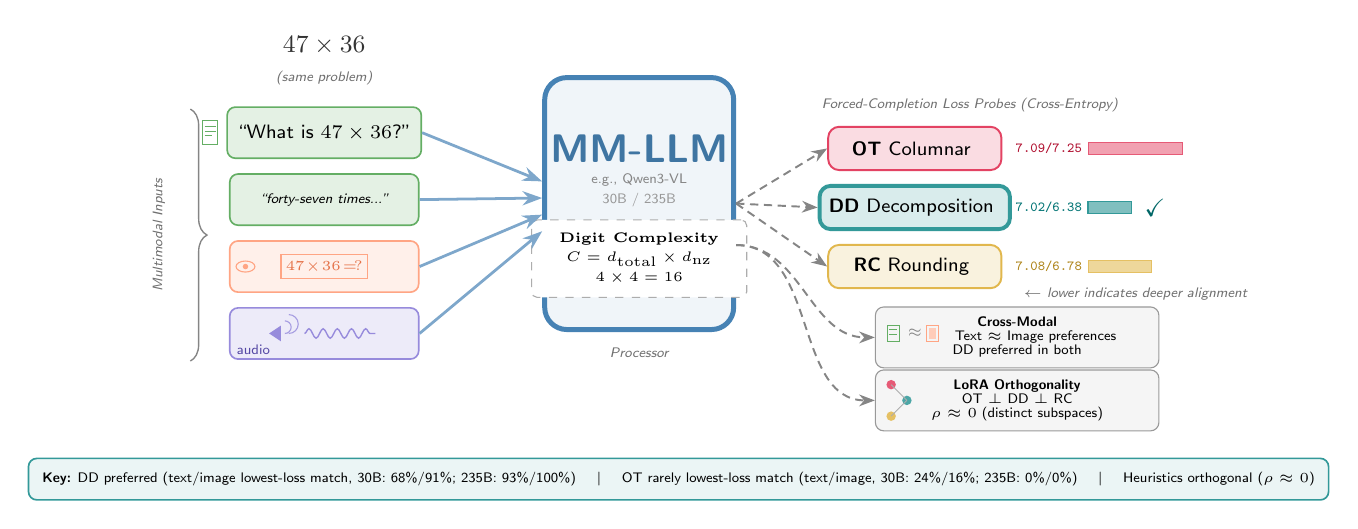
\begin{tikzpicture}[
    % Scale for ACL column width
    x=1cm, y=1cm,
    % Node styles
    modality/.style={
        rectangle,
        rounded corners=3pt,
        minimum width=2.4cm,
        minimum height=0.65cm,
        draw=#1!70,
        fill=#1!12,
        line width=0.6pt,
        font=\scriptsize\sffamily,
        align=center
    },
    llmbox/.style={
        rectangle,
        rounded corners=8pt,
        minimum width=2.4cm,
        minimum height=3.2cm,
        draw=steelblue,
        line width=1.8pt,
        fill=steelblue!8,
    },
    probe/.style={
        rectangle,
        rounded corners=4pt,
        minimum width=2.2cm,
        minimum height=0.65cm,
        draw=#1!80,
        fill=#1!15,
        line width=0.7pt,
        font=\scriptsize\sffamily,
        align=center
    },
    metricbox/.style={
        rectangle,
        rounded corners=2pt,
        draw=charcoal!40,
        dashed,
        fill=white,
        font=\tiny,
        inner sep=4pt
    },
    analysisbox/.style={
        rectangle,
        rounded corners=3pt,
        draw=charcoal!50,
        fill=charcoal!5,
        font=\tiny\sffamily,
        inner sep=3pt,
        minimum width=2.8cm
    },
    flowArrow/.style={
        ->,
        >={Stealth[length=2.5mm, width=1.8mm]},
        line width=1pt,
        steelblue!70
    },
    probeArrow/.style={
        ->,
        >={Stealth[length=2mm, width=1.5mm]},
        line width=0.7pt,
        charcoal!60,
        densely dashed
    },
    zonelabel/.style={
        font=\tiny\sffamily\itshape,
        charcoal!70
    },
    % Color definitions
    steelblue/.style={color={rgb,255:red,70;green,130;blue,180}},
    forestgreen/.style={color={rgb,255:red,34;green,139;blue,34}},
    coral/.style={color={rgb,255:red,255;green,127;blue,80}},
    slatepurple/.style={color={rgb,255:red,106;green,90;blue,205}},
    crimson/.style={color={rgb,255:red,220;green,20;blue,60}},
    teal/.style={color={rgb,255:red,0;green,128;blue,128}},
    gold/.style={color={rgb,255:red,218;green,165;blue,32}},
    charcoal/.style={color={rgb,255:red,51;green,51;blue,51}},
    indigo/.style={color={rgb,255:red,75;green,0;blue,130}},
]

% Define colors for fill operations
\definecolor{steelblue}{RGB}{70,130,180}
\definecolor{forestgreen}{RGB}{34,139,34}
\definecolor{coral}{RGB}{255,127,80}
\definecolor{slatepurple}{RGB}{106,90,205}
\definecolor{crimson}{RGB}{220,20,60}
\definecolor{teal}{RGB}{0,128,128}
\definecolor{gold}{RGB}{218,165,32}
\definecolor{charcoal}{RGB}{51,51,51}
\definecolor{indigo}{RGB}{75,0,130}

% ==========================================
% ZONE 1: INPUT MODALITIES (Left)
% ==========================================

% Problem header
\node[font=\small\bfseries, charcoal] at (0, 2.3) {$47 \times 36$};
\node[zonelabel] at (0, 1.9) {(same problem)};

% Numeric text input
\node[modality=forestgreen] (numtext) at (0, 1.2) {``What is $47 \times 36$?''};

% Text icon (small document)
\draw[forestgreen!70, line width=0.4pt] (-1.55, 1.05) rectangle (-1.35, 1.35);
\draw[forestgreen!70, line width=0.3pt] (-1.52, 1.28) -- (-1.38, 1.28);
\draw[forestgreen!70, line width=0.3pt] (-1.52, 1.22) -- (-1.38, 1.22);
\draw[forestgreen!70, line width=0.3pt] (-1.52, 1.16) -- (-1.42, 1.16);

% Alphabetic text input
\node[modality=forestgreen, font=\tiny\sffamily\itshape] (alphatext) at (0, 0.35) {``forty-seven times...''};

% Image input
\node[modality=coral] (image) at (0, -0.5) {};
% Image content: mini equation in frame
\draw[coral!70, line width=0.5pt] (-0.55, -0.65) rectangle (0.55, -0.35);
\node[font=\tiny\ttfamily, coral!90!black] at (0, -0.5) {$47\!\times\!36\!=\!?$};
% Eye icon
\draw[coral!70, line width=0.4pt] (-1.0, -0.5) ellipse (0.12 and 0.07);
\fill[coral!70] (-1.0, -0.5) circle (0.035);

% Audio input
\node[modality=slatepurple] (audio) at (0, -1.35) {};
% Speaker icon
\fill[slatepurple!70] (-0.7, -1.35) -- (-0.55, -1.25) -- (-0.55, -1.45) -- cycle;
\draw[slatepurple!60, line width=0.4pt] (-0.5, -1.35) arc (-90:90:0.08);
\draw[slatepurple!60, line width=0.4pt] (-0.45, -1.35) arc (-90:90:0.12);
% Waveform
\draw[slatepurple!70, line width=0.5pt, decorate, decoration={snake, amplitude=0.6mm, segment length=1.8mm}] (-0.25, -1.35) -- (0.65, -1.35);
\node[font=\tiny\sffamily, slatepurple!80!black] at (-0.9, -1.55) {audio};

% Brace for modalities
\draw[decorate, decoration={brace, amplitude=6pt, mirror}, charcoal!60, line width=0.5pt]
    (-1.7, -1.7) -- (-1.7, 1.5);
\node[zonelabel, rotate=90] at (-2.1, -0.1) {Multimodal Inputs};

% ==========================================
% ZONE 2: VLM PROCESSING (Center)
% ==========================================

% Main VLM box
\node[llmbox] (llm) at (4, 0.3) {};
\node[font=\Large\bfseries\sffamily, steelblue!90!black] at (4, 1.0){MM-LLM};
\node[font=\tiny\sffamily, charcoal!60] at (4, 0.6) {e.g., Qwen3-VL};
\node[font=\tiny\sffamily, charcoal!50] at (4, 0.35) {30B / 235B};

% Complexity metric box inside VLM
\node[metricbox] at (4, -0.4) {%
    \begin{tabular}{c}
    \textbf{Digit Complexity} \\[1pt]
    $C = d_{\text{total}} \times d_{\text{nz}}$ \\[1pt]
    {\tiny $4 \times 4 = 16$}
    \end{tabular}
};

% Zone label
\node[zonelabel] at (4, -1.6) {Processor};

% Flow arrows from modalities to VLM
\draw[flowArrow] (numtext.east) -- ([yshift=8pt]llm.west);
\draw[flowArrow] (alphatext.east) -- ([yshift=2pt]llm.west);
\draw[flowArrow] (image.east) -- ([yshift=-4pt]llm.west);
\draw[flowArrow] (audio.east) -- ([yshift=-10pt]llm.west);

% ==========================================
% ZONE 3: ANALYSIS PIPELINE (Right)
% ==========================================

% Analysis header
%\node[font=\scriptsize\sffamily\bfseries, charcoal] at (8.2, 2.0) {Analysis Pipeline};

% --- FORCED-COMPLETION LOSS PROBES SECTION ---
\node[zonelabel] at (8.2, 1.55) {Forced-Completion Loss Probes (Cross-Entropy)};

% OT Probe (highest loss = least preferred)
\node[probe=crimson, minimum height=0.55cm] (ot) at (7.5, 1.0) {%
    \textbf{OT} Columnar
};
% Loss value (30B/235B)
\node[font=\tiny\ttfamily, crimson!80!black] at (9.15, 1.0) {\;\;\HDSTestPerpOTThirtyB/\HDSTestPerpOTTwoThirtyFiveB};
% Bar (longest)
\fill[crimson!40] (9.7, 0.92) rectangle (10.9, 1.08);
\draw[crimson!70, line width=0.3pt] (9.7, 0.92) rectangle (10.9, 1.08);

% DD Probe (lowest loss = most preferred) - HIGHLIGHTED
\node[probe=teal, line width=1.4pt, minimum height=0.55cm] (dd) at (7.5, 0.25) {%
    \textbf{DD} Decomposition
};
% Loss value (bold - best)
\node[font=\tiny\ttfamily\bfseries, teal!90!black] at (9.15, 0.25) {\;\;\HDSTestPerpDDThirtyB/\HDSTestPerpDDTwoThirtyFiveB};
% Bar (shortest = best)
\fill[teal!50] (9.7, 0.17) rectangle (10.25, 0.33);
\draw[teal!80, line width=0.5pt] (9.7, 0.17) rectangle (10.25, 0.33);
% Checkmark
\node[font=\small, teal!80!black] at (10.55, 0.25) {\checkmark};

% RC Probe (medium loss)
\node[probe=gold, minimum height=0.55cm] (rc) at (7.5, -0.5) {%
    \textbf{RC} Rounding
};
% Loss value
\node[font=\tiny\ttfamily, gold!80!black] at (9.15, -0.5) {\;\;\HDSTestPerpRCThirtyB/\HDSTestPerpRCTwoThirtyFiveB};
% Bar (medium)
\fill[gold!45] (9.7, -0.58) rectangle (10.5, -0.42);
\draw[gold!70, line width=0.3pt] (9.7, -0.58) rectangle (10.5, -0.42);

% Bar chart legend
\node[zonelabel, font=\tiny\sffamily\itshape] at (10.3, -0.85)
{$\leftarrow$ lower indicates deeper alignment };

% Probing arrows from VLM to probes
\draw[probeArrow] (llm.east) -- (ot.west);
\draw[probeArrow] (llm.east) -- (dd.west);
\draw[probeArrow] (llm.east) -- (rc.west);

% Probe arrow label
%\node[zonelabel] at (5.8, 0.9) {\textit{Cross Entropy}};

% --- CROSS-MODAL COMPARISON SECTION ---
\node[analysisbox, minimum width=3.6cm] (crossmodal) at (8.8, -1.4) {%
    \begin{tabular}{c}
    \textbf{Cross-Modal} \\[-1pt]
    \;\;\;\;\;\;\;\;\;Text $\approx$ Image preferences \\[-1pt]
    {\tiny DD preferred in both}
    \end{tabular}
};

% Small icons for text and image
\draw[forestgreen!70, line width=0.3pt] (7.15, -1.25) rectangle (7.3, -1.45);
\draw[forestgreen!70, line width=0.2pt] (7.17, -1.3) -- (7.28, -1.3);
\draw[forestgreen!70, line width=0.2pt] (7.17, -1.36) -- (7.28, -1.36);
\node[font=\tiny, charcoal!60] at (7.5, -1.35) {$\approx$};
\draw[coral!70, line width=0.3pt] (7.65, -1.25) rectangle (7.8, -1.45);
\fill[coral!40] (7.68, -1.28) rectangle (7.77, -1.42);

% --- LoRA ORTHOGONALITY SECTION ---
\node[analysisbox, minimum width=3.6cm] (lora) at (8.8, -2.2) {%
    \begin{tabular}{c}
    \textbf{LoRA Orthogonality} \\[-1pt]
    OT $\perp$ DD $\perp$ RC \\[-1pt]
    {\tiny $\rho \approx 0$ (distinct subspaces)}
    \end{tabular}
};

% Visual: three orthogonal dots/lines
\fill[crimson!70] (7.2, -2.0) circle (0.06);
\fill[teal!70] (7.4, -2.2) circle (0.06);
\fill[gold!70] (7.2, -2.4) circle (0.06);
\draw[charcoal!40, line width=0.3pt] (7.2, -2.0) -- (7.4, -2.2);
\draw[charcoal!40, line width=0.3pt] (7.4, -2.2) -- (7.2, -2.4);

% Dashed arrows from VLM to analysis sections
\draw[probeArrow] ([yshift=-15pt]llm.east) to[out=0, in=180] (crossmodal.west);
\draw[probeArrow] ([yshift=-15pt]llm.east) to[out=0, in=180] (lora.west);

% ==========================================
% KEY FINDINGS CALLOUT (Bottom)
% ==========================================

\node[draw=teal!80, rounded corners=3pt, fill=teal!8,
      font=\tiny\sffamily, inner sep=5pt, line width=0.6pt,
      minimum width=11cm]
    at (4.5, -3.2) {%
    \textbf{Key:} DD preferred (text/image lowest-loss match, 30B: \HDSTestDDDetectionThirtyB/\HDSTestDDDetectionImageThirtyB; 235B: \HDSTestDDDetectionTwoThirtyFiveB/\HDSTestDDDetectionImageTwoThirtyFiveB) \quad $\mid$ \quad OT rarely lowest-loss match (text/image, 30B: \HDSTestOTDetectionThirtyB/\HDSTestOTDetectionImageThirtyB; 235B: \HDSTestOTDetectionTwoThirtyFiveB/\HDSTestOTDetectionImageTwoThirtyFiveB) \quad $\mid$ \quad Heuristics orthogonal ($\rho \approx 0$)
};

\end{tikzpicture}

}
\caption{
  Overview of our arithmetic benchmark and heuristic fingerprinting methodology for Multi-Modal LLMs (MM-LLMs). In the released generator, the same multiplication problem (e.g., $47 \times 36$) is paired across numeric text, rendered numeric image, and audio. The companion evaluation pipeline extends this benchmark family with broader representation variants, including alphabetic text/image conditions used in the regression figures.
  %We compute digit complexity ($C = d_{\text{total}} \times d_{\text{nz}}$) as a predictor of difficulty. Perplexity probes score relative forced-completion loss for each reasoning preamble, reflecting how compatible each heuristic is with the model's continuation distribution. Results show LLMs prefer decomposition (DD) over columnar multiplication (OT) across both Qwen sizes (Table~\ref{tab:modality-comparison}), with OT lowest-loss match rates below DD on their respective targets.
}
\label{fig:overview}
\end{figure*}


\section{Background}

\subsection{Arithmetic Reliability in LLMs}

To situate our controlled benchmark, we briefly summarize what prior work has established about exact arithmetic in LLMs and why existing evaluations do not yet provide a clean, comparable picture of arithmetic-specific failure modes. Although LLMs can produce fluent arithmetic explanations, controlled evaluations show that exact multi-digit computation remains brittle: accuracy drops quickly as digit length grows and carry interactions accumulate, and small changes in operand configuration can flip correctness even under deterministic decoding \citep{yuan2023llm-arithmetic}. Prompting methods such as chain-of-thought can improve performance on many reasoning benchmarks by eliciting intermediate steps \citep{wei2022chain}, and math-focused pretraining and verification-style training can further raise end-to-end scores on quantitative tasks \citep{lewkowycz2022minerva,cobbe2021gsm8k}.

However, these approaches still rely on the model executing intermediate arithmetic correctly, so improved benchmark performance does not imply robust arithmetic execution across scales and surface forms \citep{yuan2023llm-arithmetic}. Finally, widely used datasets such as GSM8K provide end-to-end correctness labels for word problems, entangling language understanding, planning, and computation in a way that makes arithmetic-specific failure modes difficult to isolate \citep{cobbe2021gsm8k}.

\subsection{Representation and Modality Effects}

Beyond operand size and carry interactions, arithmetic success is also sensitive to how the same computation is encoded and delivered to the model. Arithmetic questions increasingly arrive in diverse formats---typed numerals, number words, and multimodal inputs such as screenshots or rendered equations---as foundation models extend from text-only to vision-language interfaces \citep{alayrac2022flamingo,openai2023gpt4v}. Recent multimodal benchmarks and instruction-tuned systems target broad mathematical reasoning in visual contexts \citep{lu2023mathvista,chen2024mathllava}, but they typically emphasize heterogeneous problem types and rich visual scenes rather than isolating \emph{basic arithmetic} under controlled structural variation. As a result, it remains unclear how much multimodal degradation reflects perceptual/representation noise versus limitations in the underlying computation \citep{liu2024ocrbench}, and whether failures transfer systematically across modalities when the arithmetic itself is held fixed \citep{lu2023mathvista,chen2024mathllava}.

\subsection{Arithmetic Heuristics and Strategy Probing}

Even when the input format is held fixed, multiplication can be carried out via multiple procedures, and strategy choice changes both intermediate operation counts and characteristic error modes. Work in mathematical cognition emphasizes that multiplication is supported by multiple strategies rather than a single uniform procedure; strategy choice depends on operand structure, experience, and context \citep{campbell2005cognitive,dehaene2011number}. Three canonical heuristics that make distinct predictions about difficulty and error structure are:
\begin{itemize}
    \item \textbf{Columnar / long multiplication (OT)}: compute digit-by-digit partial products with explicit carry propagation (the standard schoolbook algorithm), e.g., multiply by the ones digit, then by the tens digit, and add shifted partial products \citep{campbell2005cognitive}.
    \item \textbf{Distributive decomposition (DD)}: rewrite an operand as a sum and add partial products, e.g., $47 \times 36 = 40 \times 36 + 7 \times 36$ \citep{campbell2005cognitive,dehaene2011number}.
    \item \textbf{Rounding--compensation (RC)}: round to a convenient base and correct, e.g., $49 \times 51 = (50-1)(50+1) = 50^2 - 1$ \citep{campbell2005cognitive}.
\end{itemize}
These heuristics imply different computational burdens (number of partial products, carries, and adjustments) and characteristic failure modes when steps are omitted or misapplied \citep{campbell2005cognitive,dehaene2011number}.

More broadly, probing methods in NLP offer tools for testing which representations or computations are most compatible with a model \citep{belinkov2022probing}. In our setting, we operationalize strategy preference by comparing the model-likelihood of heuristic-specific reasoning prefixes, and we complement this with parameter-efficient adaptation (LoRA) to study whether strategy-specialized updates align or separate in parameter space \citep{hu2022lora}. We hypothesize that multimodal LLMs exhibit systematic preferences among arithmetic heuristics, and that these preferences help explain predictable patterns of breakdown as digit structure and modality vary.

\section{Methodology}

\subsection{Problem Design}

Building on the evidence above that arithmetic failures depend on both operand structure and surface form, we design a controlled multiplication benchmark that lets us vary these factors independently. We study multiplication in a controlled setting by generating operand pairs from digit templates that vary the number and arrangement of non-zero digits. Concretely, we sample problems from the template family shown in Table~\ref{tab:digit_templates}, which spans fully dense numbers (e.g., DD, DDD) as well as structured sparsity through trailing zeros (e.g., D0, D00, DD0) and non-adjacent non-zeros (e.g., D0D). This design lets us vary arithmetic difficulty without changing the task format, and it yields a broad range of carry patterns and intermediate-step requirements.

\begin{table}[t]
    \centering
    \small
    \begin{tabular}{ll}
        \hline
        Template & Description \\
        \hline
        D & single random digit (1--9) \\
        DD & two random digits \\
        DDD & three random digits \\
        D0, D00, DD0 & trailing zeros (reduced effective operations) \\
        D0D & non-adjacent non-zero digits \\
        \hline
    \end{tabular}
    \caption{Digit templates used to systematically control operand structure.}
    \label{tab:digit_templates}
\end{table}

To quantify difficulty with a single interpretable scalar, we define digit complexity as
\begin{equation}
    \text{Complexity}(a, b) = d_{\text{total}} \times d_{\text{non-zero}},
    \label{eq:complexity}
\end{equation}
where $d_{\text{total}}$ is the total number of digits across both operands and $d_{\text{non-zero}}$ is the count of non-zero digits. For example, $47 \times 36$ has $d_{\text{total}} = 4$ and $d_{\text{non-zero}} = 4$, yielding complexity $=16$. The motivation is practical rather than purely formal: digit complexity is a simple proxy for the number of elementary digit multiplications/additions a procedural solver would execute, and empirically it serves as a strong predictor of failure as carries and intermediate-state demands grow. This complexity score is a simple, though noisy, proxy for operation count; see Appendix~\ref{sec:formal-notes}.

\subsection{Model Configuration}

With the problem distribution fixed, we next specify the model families we use to (i) measure multimodal arithmetic accuracy at scale and (ii) run token-level probes and adaptations that require access to cross-entropy losses. We use two complementary pipelines. The multimodal accuracy/regression analyses are generated in a separate companion codebase that evaluates Gemini 2.5 Flash plus matched Qwen runs on the shared benchmark family. The repository released here covers the paired benchmark generator and the Qwen3-VL-30B-A3B-Instruct / Qwen3-VL-235B-A22B-Instruct fingerprinting, behavioral nudge, and adapter-geometry experiments. We therefore report the Qwen sizes side-by-side (30B/235B) for the probing and LoRA analyses, while the broader multimodal accuracy curves are imported from the companion pipeline.

\subsection{Multimodal Evaluation}
To isolate modality effects, we evaluate the same underlying multiplication items while varying only the input channel. The paired benchmark generator in this repository creates \MultimodalProblemCount{} shared multiplication instances, each rendered as text, an image, and audio; the companion evaluation pipeline also includes broader representation variants used in the regression figures. For the Qwen models, we evaluate the text and image modalities (no audio). The regression tables, residual analyses, and \(R^2\)-style predictive summaries referenced later are therefore downstream artifacts from the companion benchmark codebase, while the paired problem grid itself is generated here.

We next quantify degradation with increasing difficulty by fitting, separately per modality, a logistic regression that predicts correctness from digit complexity:
\begin{equation}
    P(\text{correct}) = \sigma(\beta_0 + \beta_1 \cdot \text{Complexity}),
\end{equation}
where $\sigma$ is the logistic function. This formulation highlights digit complexity as a compact predictor comparable across problem families.

\paragraph{Error-rate model.} If each primitive digit operation fails independently with probability $p$, then $P(\text{correct}) \approx (1-p)^{N_{\text{ops}}} \approx \exp(-p N_{\text{ops}})$, so log-accuracy is linear in the operation count. We use logistic regression as a convenient monotone fit across modalities; its slope should be read as an empirical difficulty parameter rather than a literal per-operation error rate. A log link on $P(\text{correct})$ matches the independent-error approximation; other monotone links (including complementary log-log) can be reasonable under different parameterizations of $N_{\text{ops}}$ (see Appendix~\ref{sec:formal-notes}).

\subsection{Heuristic Fingerprinting via a Perplexity Probe}
Accuracy-versus-complexity curves tell us \emph{when} models break down, but they do not by themselves reveal \emph{which} intermediate procedure the model is predisposed to follow on a given instance. To probe which procedural strategy a model finds most ``natural'' for a given multiplication instance \citep{belinkov2022probing}, we introduce a perplexity-style loss probe implemented with Qwen3-VL-30B-A3B-Instruct and Qwen3-VL-235B-A22B. We infer heuristic preference from relative loss under forced continuation (token-level cross-entropy), avoiding costly and often noisy free-form generation; this enables large-scale preference measurement with stable compute and without confounds from sampling, verbosity, or post-hoc answer formatting.

For each problem $(a,b)$ we construct a small bank of \emph{heuristic-conditioned} assistant continuations, each describing a specific computation style in short, operand-free language so that the same template bank can be applied to matched text and image presentations:
\begin{itemize}
    \item \textbf{OT}: ``Column method: start with the ones digits''
    \item \textbf{DD}: ``Decomposition: split one factor into place-value parts''
    \item \textbf{RC}: ``Round and adjust: use a nearby round base, then compensate''
\end{itemize}
To ensure that loss differences reflect genuine heuristic alignment rather than superficial artifacts, the default probe uses a balanced bank of short, stylistically matched paraphrases per heuristic together with a neutral baseline preamble so that we can report relative preferences as $\Delta$loss rather than raw loss. We score each heuristic by the length-normalized cross-entropy of its continuation tokens under the same question context (forced completion), averaging across the active template bank, and we interpret \emph{lower} loss (or more negative $\Delta$loss relative to the neutral prompt) as a deeper alignment with that heuristic's initial reasoning trajectory. We treat the minimum-loss aggregated template bank as a per-instance, loss-based label and analyze how both labels and margins shift with operand cues and modality. Detection confidence in the tables is the margin-based quantity
\[
\mathrm{conf} = \min\!\left(1,\; 2 \cdot \frac{\ell_{(2)} - \ell_{(1)}}{\ell_{(2)}}\right),
\]
where $\ell_{(1)}$ and $\ell_{(2)}$ are the lowest and second-lowest aggregated losses. The released probe code also supports explicit style-mismatch ablations; the results reported here use the default balanced template bank unless noted otherwise. All prompts are wrapped in the model's chat template\footnote{For images, including vision markers.} and we compute loss only on the heuristic preamble/continuation tokens.

\paragraph{Likelihood-ratio view.} Let $\ell(h)$ be the length-normalized cross-entropy over the heuristic template continuation tokens under the same question context (forced completion), and let $\ell_0$ be the neutral baseline. If templates are token-length matched with length $T$, then $-T \Delta \ell(h)$ equals the log-likelihood ratio between candidate templates under the same model and context, and choosing the minimum-loss heuristic is the maximum-likelihood choice under equal priors. When lengths differ, $\Delta \ell$ should be read as a normalized naturalness score rather than an exact decision rule (see Appendix~\ref{sec:formal-notes}).

A second novelty enabled by this probing setup is cross-modal heuristic comparison: because Qwen is vision-language, we can apply the same loss-based heuristic scoring to matched text and rendered-image presentations of the \emph{same} underlying multiplication problems. This lets us test whether the model's preferred strategy shifts when the input modality changes, without relying on post-hoc rationales or chain-of-thought extraction.

We evaluate the probe on two complementary datasets we construct to stress discriminative strategy prediction while preventing leakage. The current canonical release is the versioned Heuristic-Disagreement Set (HDSv2), which contains \HDSAllCount{} problems intentionally chosen so that different heuristics make competing predictions about an efficient approach (e.g., near-base numbers where RC is attractive) but labeled by an explicit symmetric OT/DD/RC cost model rather than by hand-tuned applicability scores. Each item stores both a \emph{design family} (the construction bucket used to generate the problem) and a \emph{canonical target heuristic} (the minimum-cost heuristic under the cost model). We enforce uniqueness up to commutativity and split HDS into train/validation/test using \DatasetSplitRatios{}. The current split composition is \HDSTrainCount{}/\HDSValCount{}/\HDSTestCount{} items, with per-family counts (\HDSTrainRCCount{}, \HDSTrainDDCount{}, \HDSTrainOTCount{}) / (\HDSValRCCount{}, \HDSValDDCount{}, \HDSValOTCount{}) / (\HDSTestRCCount{}, \HDSTestDDCount{}, \HDSTestOTCount{}). Separately, we include Adversarial Traps (\TrapsCount{} problems) that target known weaknesses of particular heuristics (e.g., cascading carries that stress OT); these are always held out as test-only and are constructed to be disjoint from HDS. Unless otherwise stated, we report metrics on the held-out test split only, ensuring that any template tuning or adapter training cannot inadvertently optimize on evaluation instances.

Table~\ref{tab:hds-snippet} shows a small snippet of HDS entries, illustrating the operand structure, target heuristic, and category labels used in the dataset.

\begin{table}[t]
  \centering
  \small
  \begin{tabular}{llll}
    \hline
    ID & Problem & Target & Category \\
    \hline
    hds\_000 & $49 \times 51 = 2499$ & RC & \texttt{near\_50\_sym} \\
    hds\_002 & $99 \times 101 = 9999$ & RC & \texttt{near\_100\_sym} \\
    hds\_009 & $47 \times 60 = 2820$ & DD & \texttt{zero\_factor} \\
    hds\_014 & $37 \times 100 = 3700$ & DD & \texttt{hundred\_factor} \\
    hds\_018 & $87 \times 96 = 8352$ & OT & \texttt{carry\_heavy} \\
    hds\_019 & $79 \times 68 = 5372$ & OT & \texttt{carry\_heavy} \\
    \hline
  \end{tabular}
  \caption{
    Snippet of HDS examples showing operands, target heuristics, and category labels. Data available at \url{https://huggingface.co/datasets/<redacted>}
  }
  \label{tab:hds-snippet}
\end{table}

\paragraph{Heuristic cost formalization.} We define simple cost models for OT/DD/RC based on digit multiplications (including by zero digits) and additions (formal definitions in Appendix~\ref{sec:formal-notes}). In the current HDSv2 release, these cost models are used directly for canonical labeling: we keep only instances where the minimum-cost heuristic is uniquely separated from the runner-up by a fixed margin, and we report lexical fingerprint results as cue-compatibility by design family rather than as direct heuristic ``accuracy.''

\subsection{Adapter Weight Orthogonality Analysis}

Because loss-based preferences could in principle reflect shallow prompt familiarity rather than genuinely distinct computations, we additionally connect strategy differences to parameter space. To test whether different heuristics correspond to meaningfully distinct computational mechanisms (rather than superficial prompt-following), we train separate LoRA adapters \citep{hu2022lora} for Qwen3-VL-30B and Qwen3-VL-235B using synthetic reasoning traces generated with no overlap with the held-out test problems. For each model we train three heuristic adapters (RC, DD, OT) plus a STYLE control adapter trained on generic reasoning-trace formatting without heuristic-specific intermediate arithmetic. The three heuristic adapters drive the main nudge and pairwise geometry analyses, while STYLE serves as a control for whether any degradation is heuristic-specific or a broader trace-steering effect. We train the heuristic adapters with early stopping on validation loss\footnote{For 30B: RC $n=\LoRARCTrainNThirtyB$ train, $\LoRARCValNThirtyB$ val; DD $n=\LoRADDTrainNThirtyB$ train, $\LoRADDValNThirtyB$ val; OT $n=\LoRAOTTrainNThirtyB$ train, $\LoRAOTValNThirtyB$ val; for 235B: RC $n=\LoRARCTrainNTwoThirtyFiveB$ train, $\LoRARCValNTwoThirtyFiveB$ val; DD $n=\LoRADDTrainNTwoThirtyFiveB$ train, $\LoRADDValNTwoThirtyFiveB$ val; OT $n=\LoRAOTTrainNTwoThirtyFiveB$ train, $\LoRAOTValNTwoThirtyFiveB$ val.}, keeping the base model fixed and learning only low-rank updates.

For each adapter we compute the effective update $\Delta W_h = B_h A_h$ across all LoRA modules (with expert dimensions handled per expert) and flatten $\Delta W_h$ into a vector, then compute pairwise cosine similarity,
\begin{equation}
    \text{sim}(h_1, h_2) = \frac{\Delta W_{h_1} \cdot \Delta W_{h_2}}{\|\Delta W_{h_1}\| \|\Delta W_{h_2}\|}.
\end{equation}
Near-zero similarity is consistent with the learned updates occupying approximately orthogonal directions in parameter space. We additionally compare each heuristic adapter against a same-heuristic seeded rerun in Appendix~\ref{tab:similarity-seed-controls}; higher same-heuristic alignment than the primary cross-heuristic baseline supports that the low-similarity signal is not just a high-dimensional artifact. Because $\Delta W$ is invariant to the LoRA factorization, this provides an invariant proxy for separability that complements behavioral probing, linking heuristic-level behavior to separable parameter-space structure.

\section{Results}

With the benchmark, modalities, and probing setup defined, we now report empirical results and use a consistent notation when comparing models. Unless otherwise noted, we report paired Qwen3-VL values as 30B / 235B, each with its standard error ($\pm$SE) across problem instances.

\subsection{Complexity Degrades Accuracy Across Modalities}

We begin by establishing a baseline for how structural difficulty dictates performance, addressing our first research question regarding the interaction of digit length and complexity. Figure~\ref{fig:complexity} shows logistic regression curves for probability of correct answer versus digit complexity across all modalities. Accuracy declines monotonically with complexity across modalities, but the ordering depends on representation and model. For Gemini, image numerical is comparable to numeric text, alphabetic text is slightly lower, and image alphabetic and audio degrade earliest. For Qwen, text remains strongest and both image variants lag; the weaker image condition flips between sizes (image numerical for 30B, image alphabetic for 235B). Across the companion accuracy pipeline, the curves approach near-zero accuracy at the highest observed difficulty levels, and the non-text conditions exhibit steeper drops that signal earlier degradation, most prominently for image alphabetic and audio in Gemini.

\begin{figure*}[ht]
  \centering
  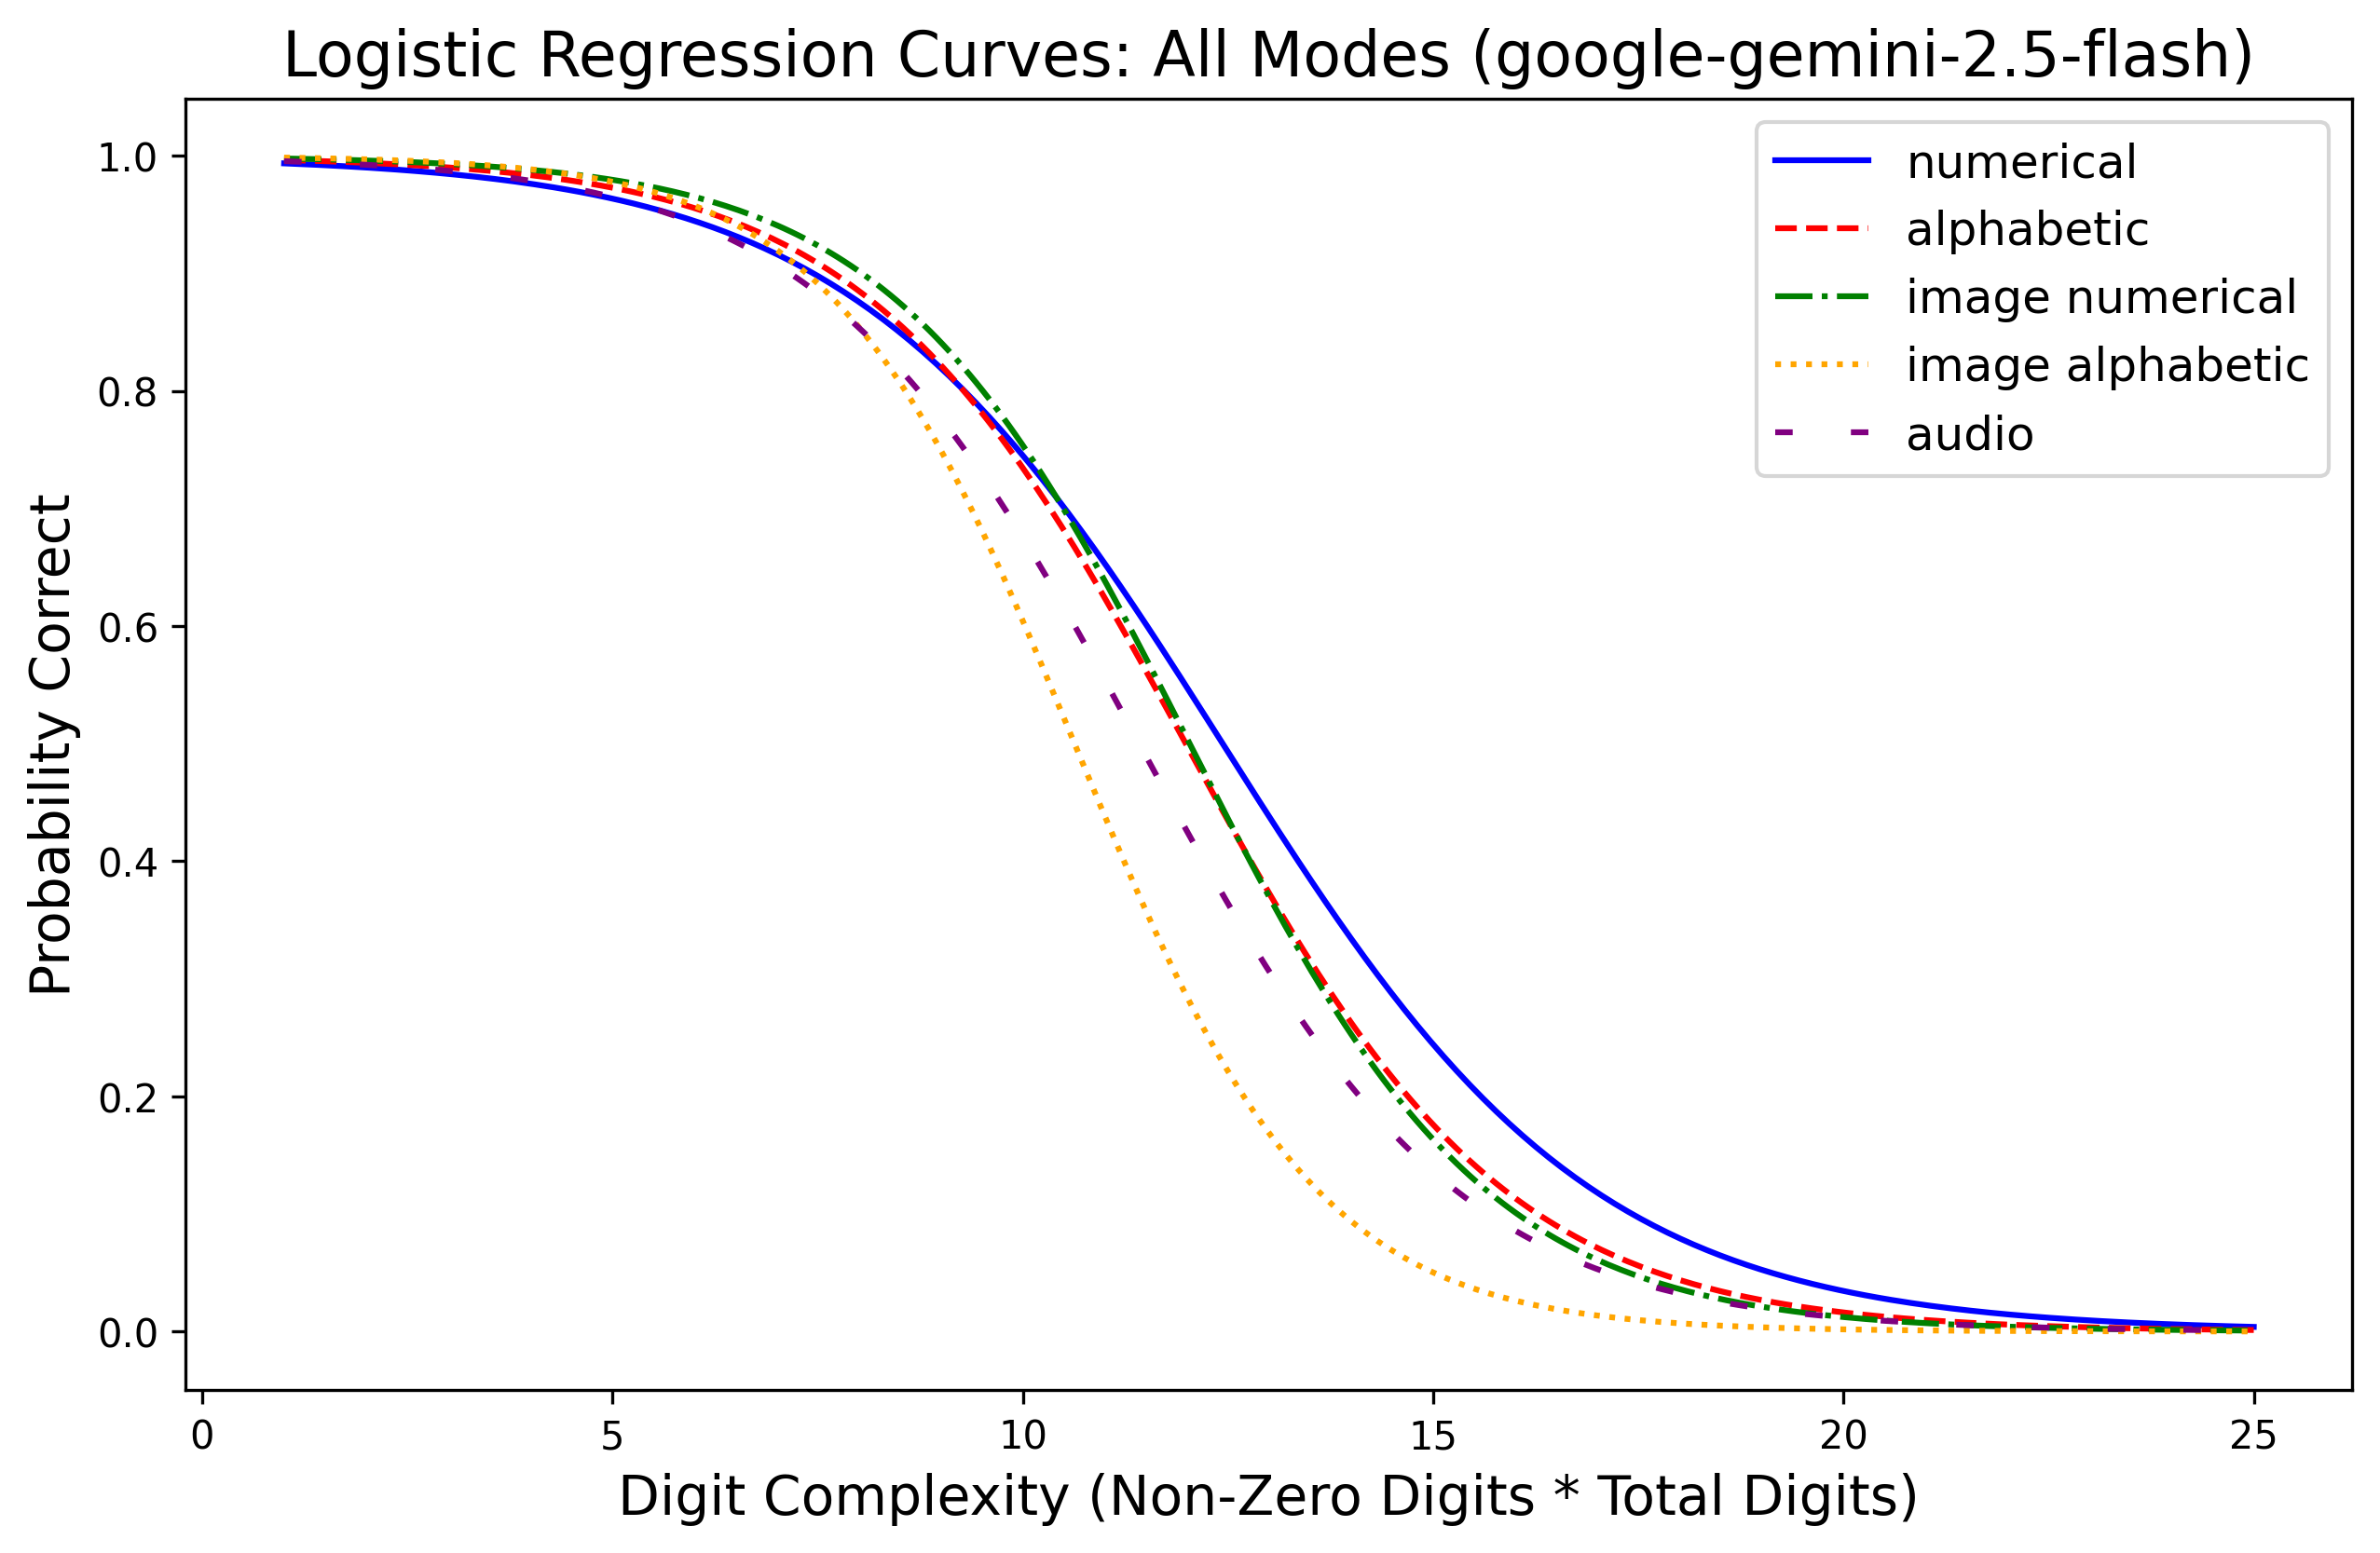
\includegraphics[width=0.65\columnwidth]{Figures/sb_logistic-regression-gemini.png}
    \vspace{0.6em}
  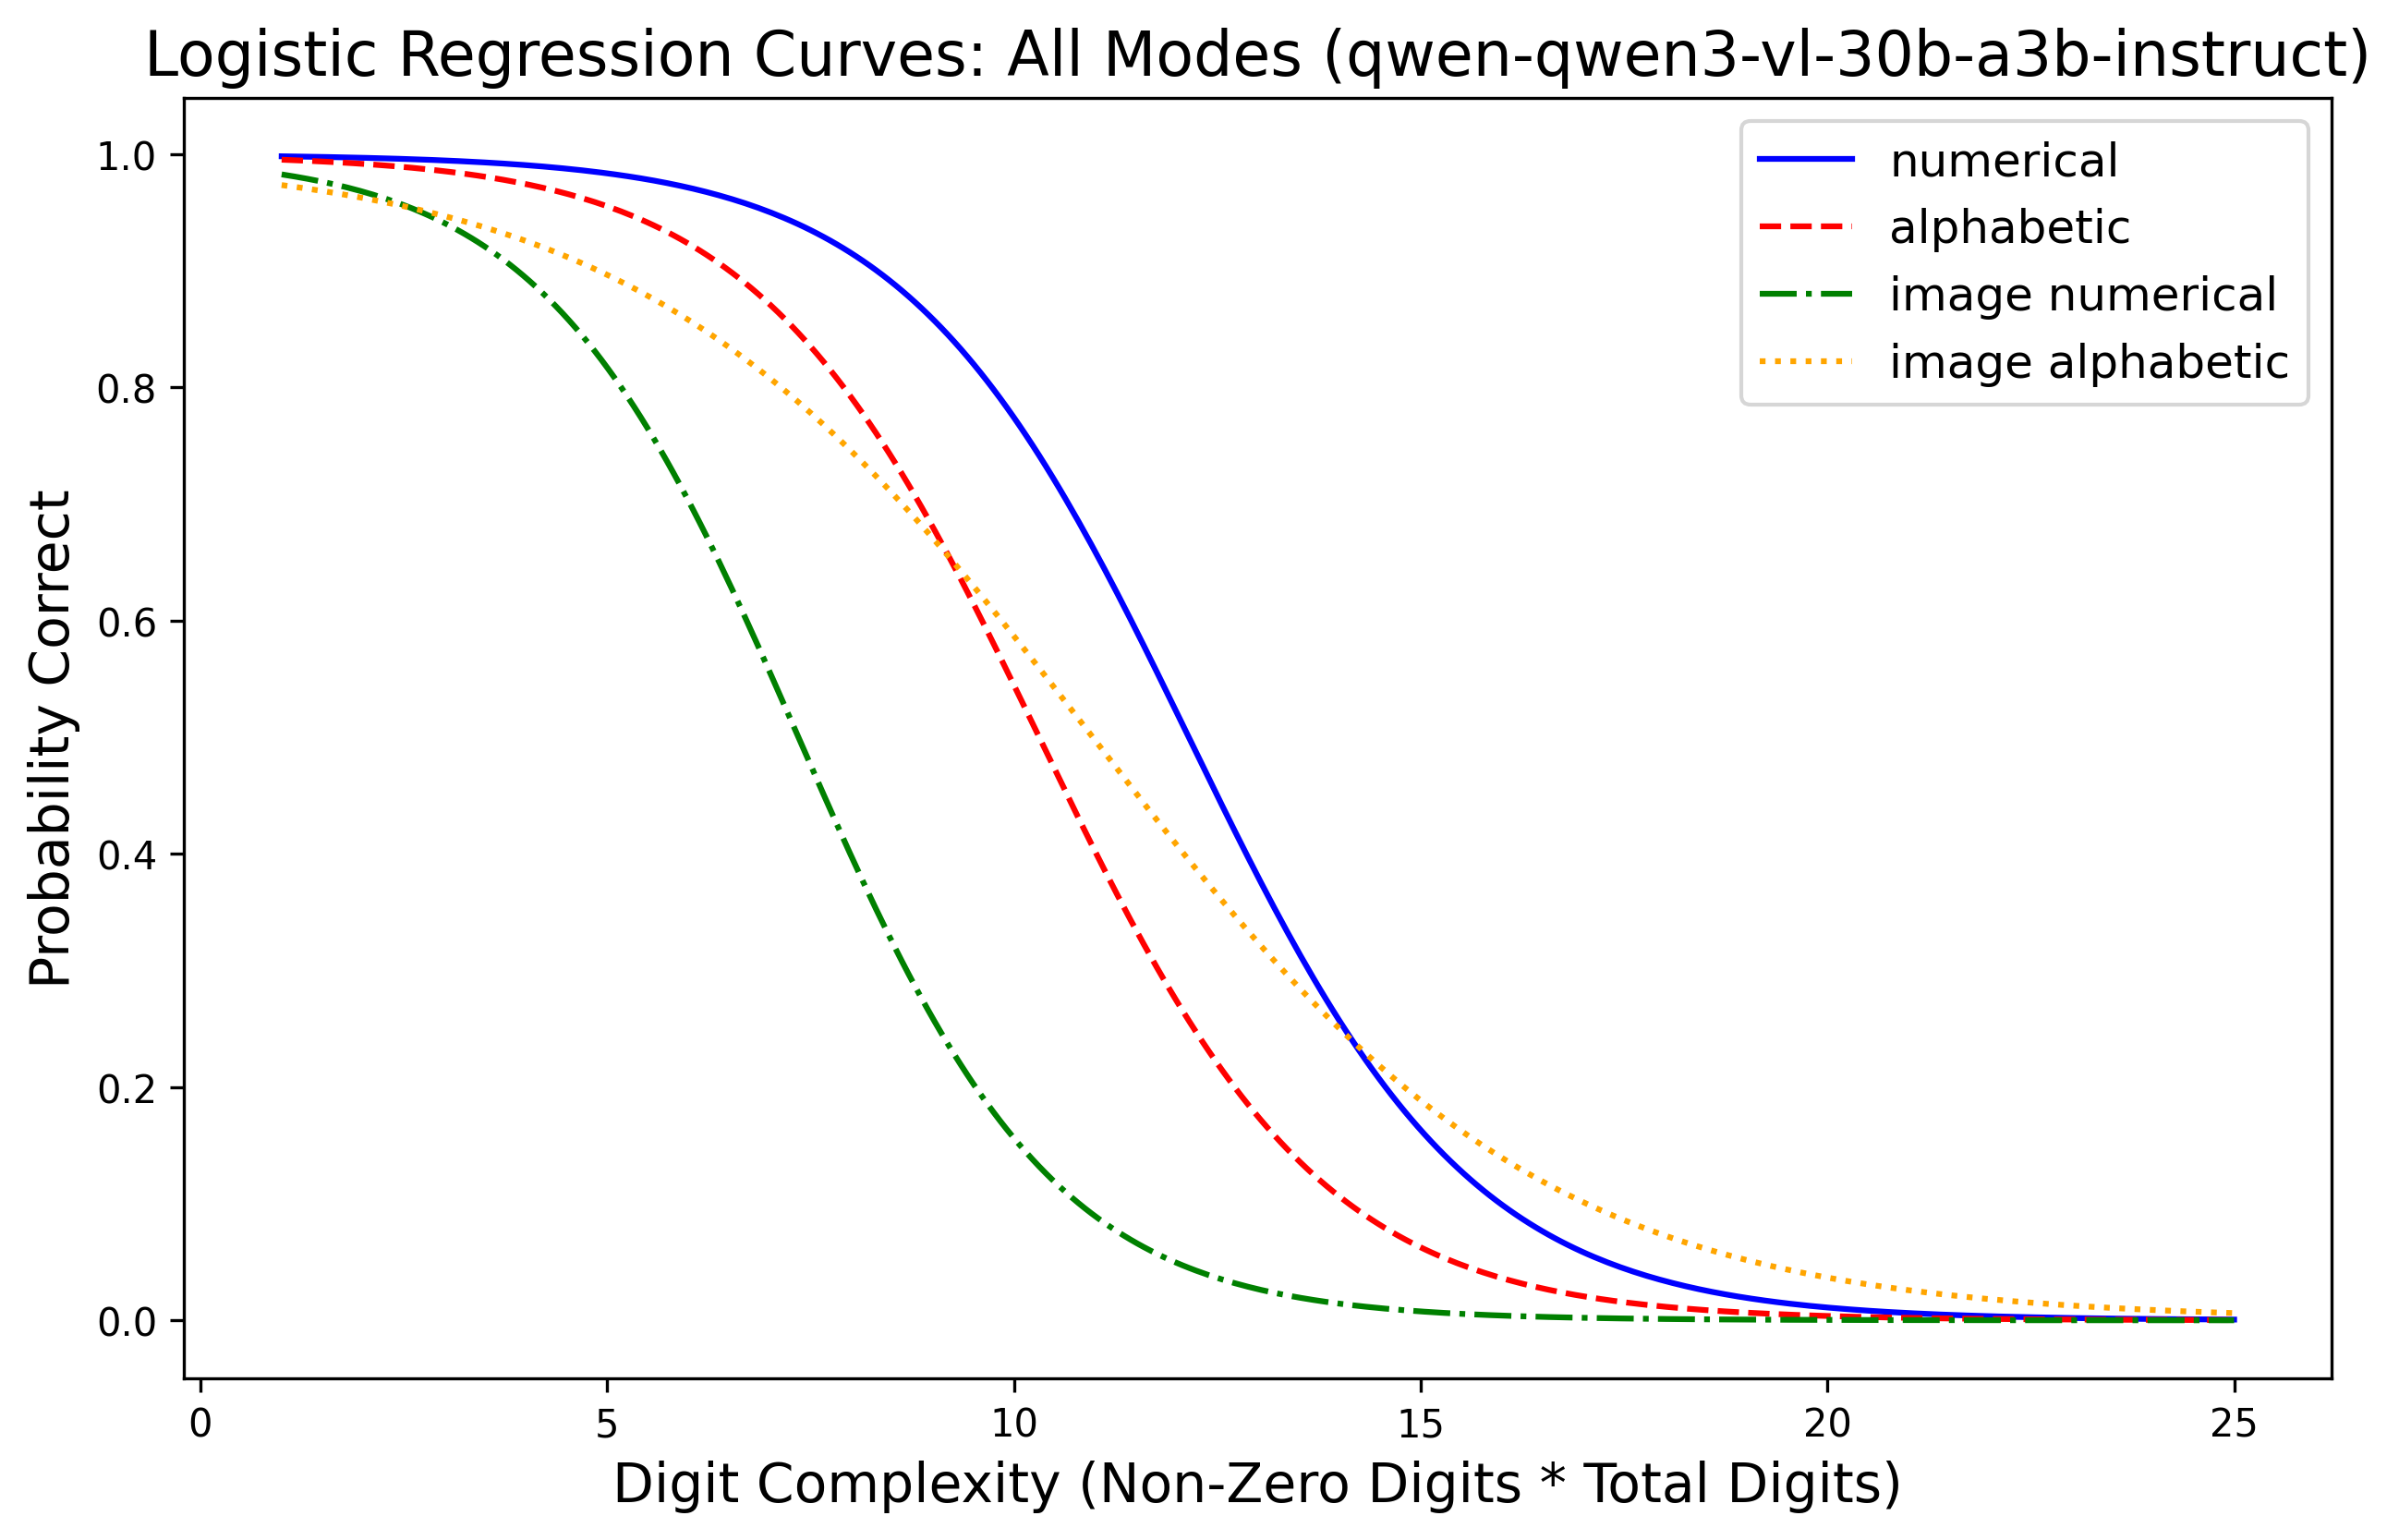
\includegraphics[width=0.65\columnwidth]{Figures/sb_logistic-regression-qwen30B.png}
  \vspace{0.6em}
  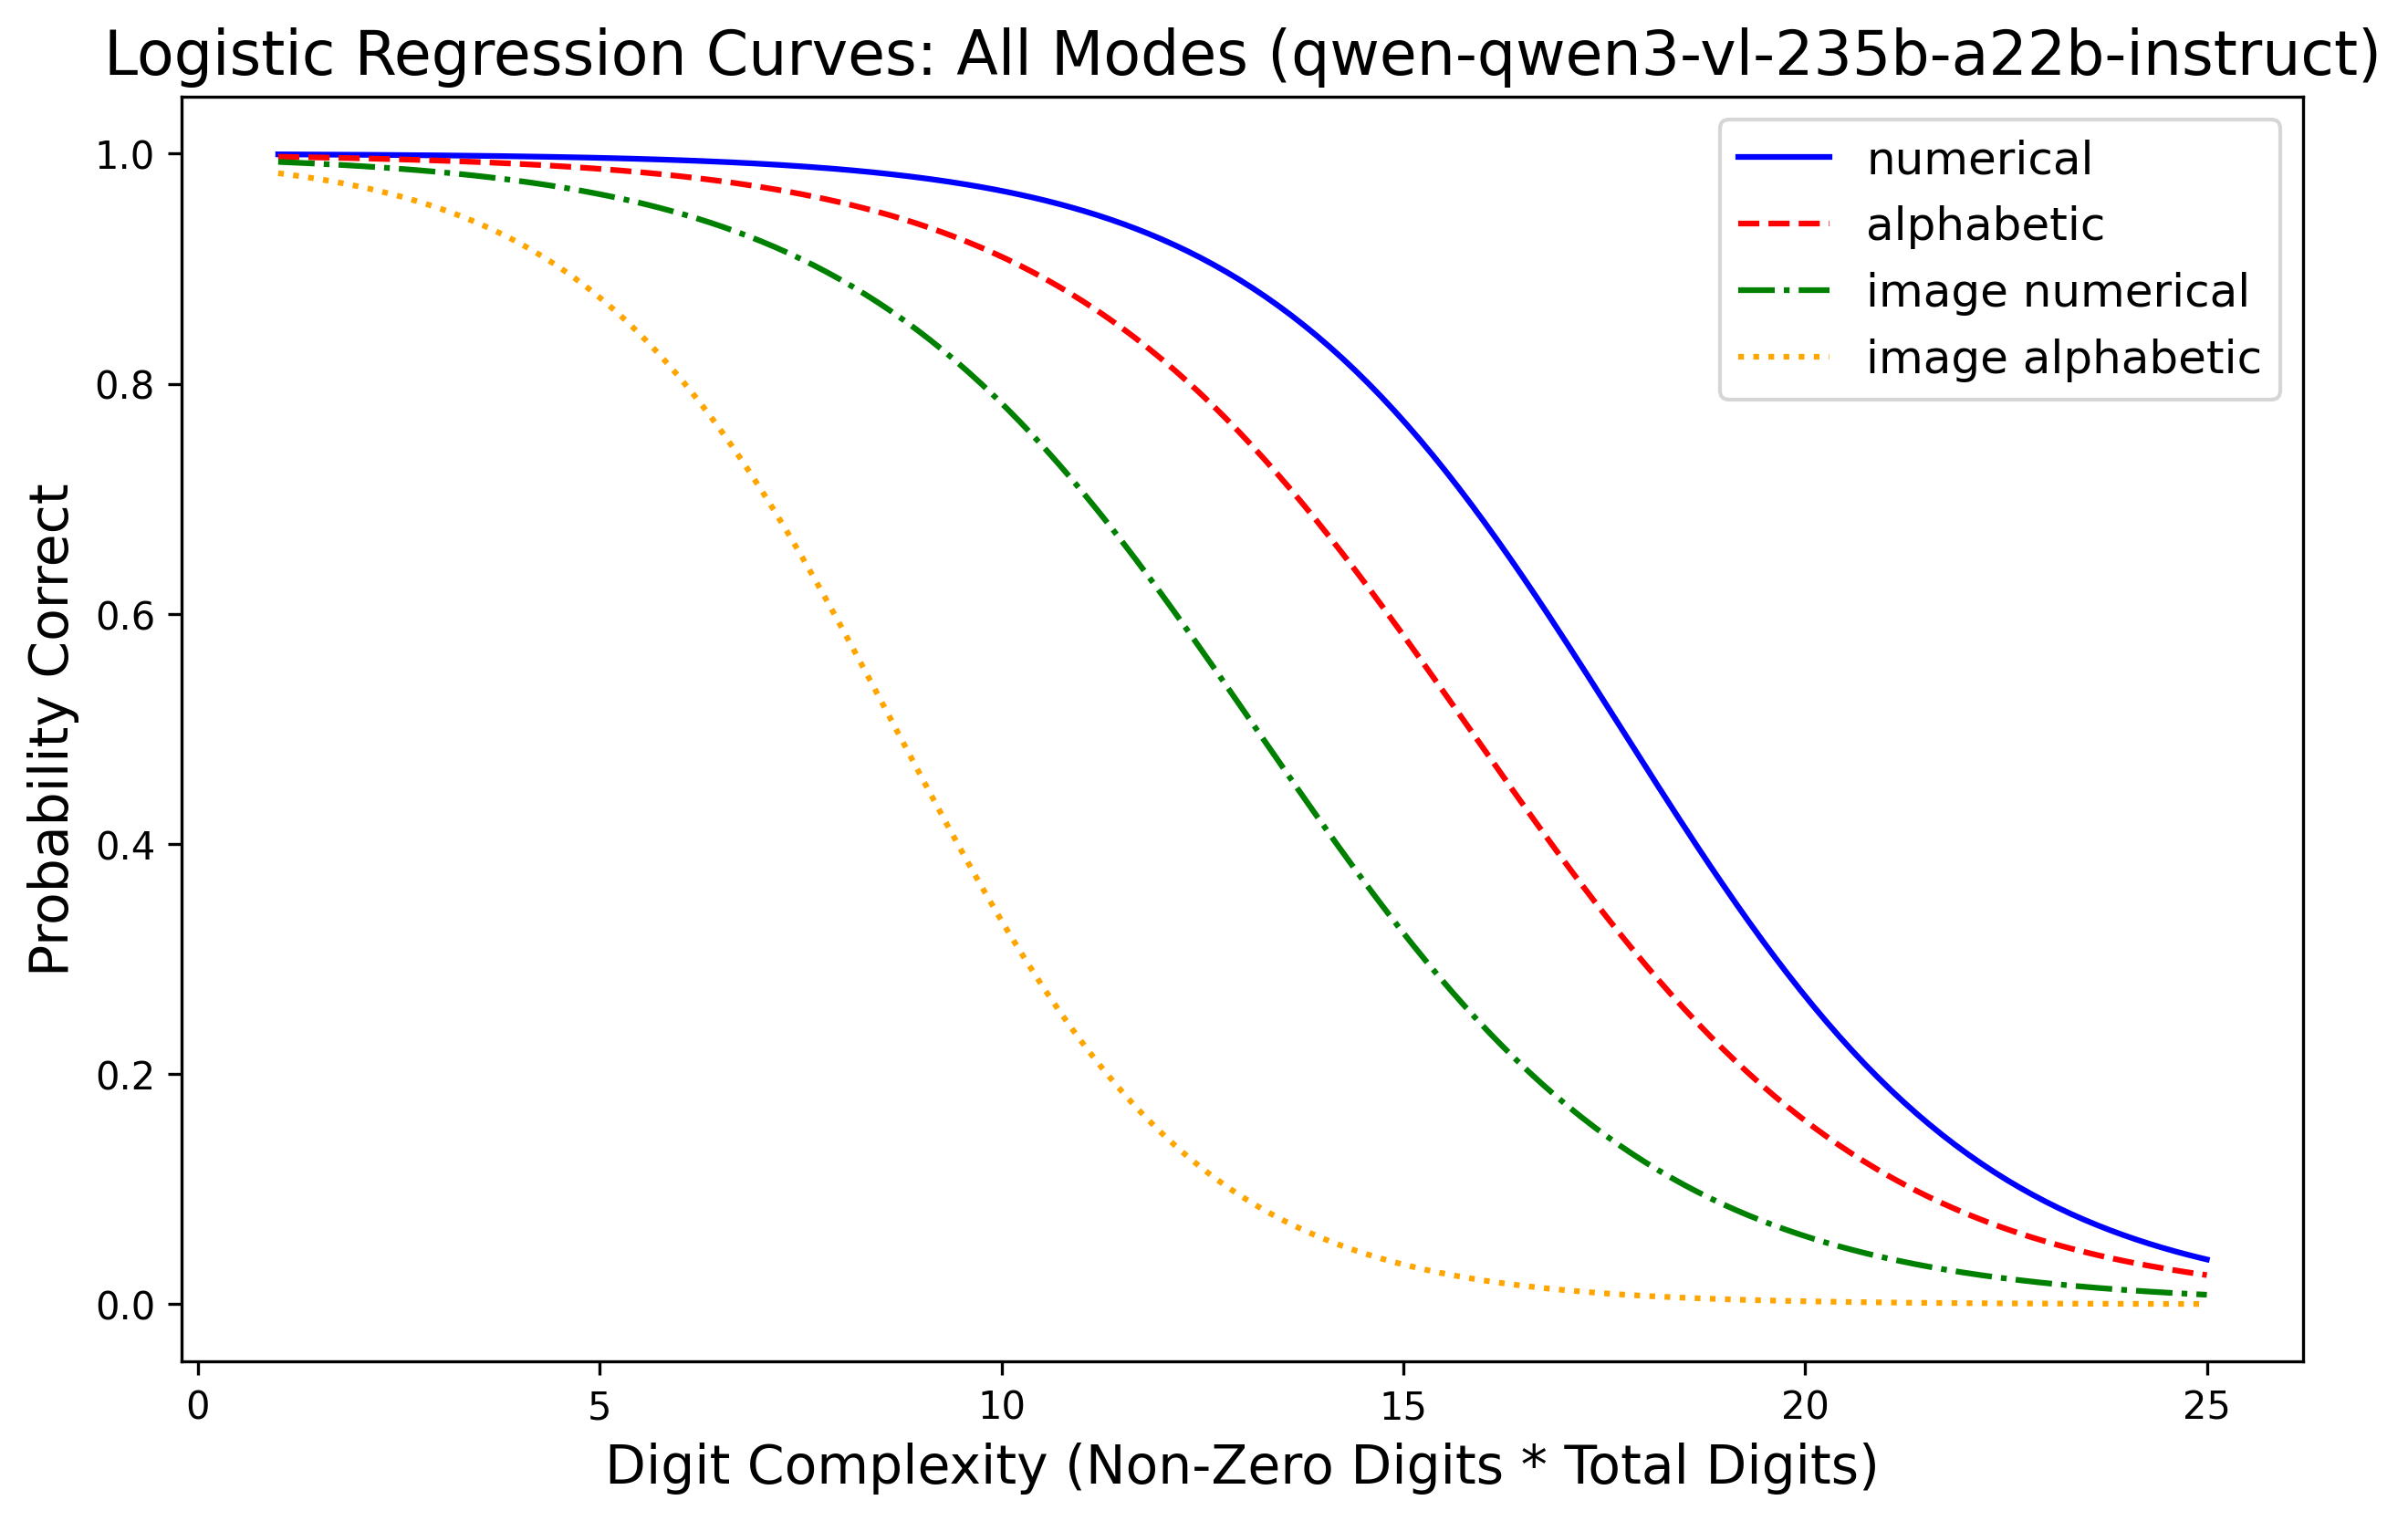
\includegraphics[width=0.65\columnwidth]{Figures/sb_logistic-regression-qwen235B.png}
  \caption{
Probability of correct multiplication answer as a function of digit complexity (total digits $\times$ non-zero digits) across input modalities for Gemini 2.5 Flash (top), Qwen3-VL-30B (middle), and Qwen3-VL-235B (bottom). Curves show fitted logistic regression models for numeric/alphabetic text, image renderings of those prompts, and audio for Gemini; Qwen uses numeric/alphabetic text and image renderings of both (no audio). See also \S\ref{sec:complexity-fits}. 
  }
  \label{fig:complexity}
\end{figure*}

To verify that this pattern is not specific to Gemini, we fit the same logistic model to Qwen3-VL-30B and Qwen3-VL-235B on numeric/alphabetic text and their image renderings (no audio). Appendix~\ref{sec:complexity-fits} reports the corresponding curves and supplementary coefficient tables that separate total digits from non-zero digit counts.

For Gemini, image alphabetic is the weakest curve, with audio close behind, plausibly because both conditions impose additional encoding and buffering demands beyond clean numeric text within the neural processing. 

Digit complexity is also mechanistically suggestive rather than purely correlational. Under decomposition/partial-product heuristics, each non-zero digit in the multiplier induces an additional (approximately full-length) partial product and carry interactions, so the required number of intermediate computations grows roughly with total digits $\times$ non-zero digits. This motivates probing which heuristic templates the model finds most natural, and whether modality shifts these preferences in ways that mirror the modality-specific degradation observed above.

\subsection{LLMs Prefer Decomposition?}

To test whether the digit-complexity effect reflects the model's reliance on a particular computation strategy (e.g., partial products vs.\ column-wise carries), we compare how well heuristic-specific preambles match the model's continuation distribution via a forced-completion loss probe.

Table~\ref{tab:modality-comparison-alt} reports mean $\Delta$loss relative to the neutral baseline on a shared held-out probe split (values $<$ 0 indicate lower forced-completion loss than neutral), resolved-probe coverage, and target support among resolved probes. Here target support is the normalized $\exp(-\ell)$ share assigned to the target heuristic when DD, RC, OT, and the neutral baseline are treated as competing continuations, so we no longer force a heuristic winner when every heuristic cue is worse than neutral.

The canonical JSONL recomputation yields a model-specific pattern. For 30B, RC has the most negative $\Delta$loss in both text and image (\HDSTestDeltaRCAltThirtyB{} / \HDSTestDeltaRCImageAltThirtyB{}), with DD and OT less negative. For 235B, DD has the smallest positive $\Delta$loss in both text and image (\HDSTestDeltaDDAltTwoThirtyFiveB{} / \HDSTestDeltaDDImageAltTwoThirtyFiveB{}), while OT is the least compatible continuation (\HDSTestDeltaOTAltTwoThirtyFiveB{} / \HDSTestDeltaOTImageAltTwoThirtyFiveB{}). The support statistics are likewise model-specific: 30B places the largest resolved-probe target support on RC-targeted items (\HDSTestRCTargetSupportAltThirtyB{} $\pm$ \HDSTestRCTargetSupportAltSEThirtyB{} / \HDSTestRCTargetSupportImageAltThirtyB{} $\pm$ \HDSTestRCTargetSupportImageAltSEThirtyB{}), whereas 235B places the largest resolved-probe target support on DD-targeted items (\HDSTestDDTargetSupportAltTwoThirtyFiveB{} $\pm$ \HDSTestDDTargetSupportAltSETwoThirtyFiveB{} / \HDSTestDDTargetSupportImageAltTwoThirtyFiveB{} $\pm$ \HDSTestDDTargetSupportImageAltSETwoThirtyFiveB{}). We report coverage separately because image probe failures previously confounded target-family comparisons; the image analyses should therefore be read through both their resolved coverage (\HDSTestResolvedCoverageImageAltThirtyB{} / \HDSTestResolvedCoverageImageAltTwoThirtyFiveB{}) and their support values. Raw cross-entropy losses with SE and Traps comparisons are reported in Appendix~\ref{sec:raw-loss}.

%\subsection{Heuristic Preferences Differ by Modality}

%We apply forced-completion loss fingerprinting to both text and image inputs by rendering the same HDS problems as LaTeX images and scoring the same heuristic templates with Qwen3-VL-30B and Qwen3-VL-235B. Table~\ref{tab:modality-comparison} reports modality-specific $\Delta$loss (forced-completion loss relative to a neutral baseline computed within each modality, so values should be compared within, not across, modalities) and shows a modest reweighting of heuristic margins; note these are synthetic renderings rather than natural images.

  \begin{table*}[ht]
    \centering\small
    \begin{tabular}{llcc}
      \hline
      \textbf{Metric} & \textbf{Model} & \textbf{Text} & \textbf{Image} \\
      \hline
      \HDSProbeAccuracyMeanCLabel{} & 30B & \HDSTestAccuracyAltThirtyB{} $\pm$ \HDSTestAccuracyAltSEThirtyB{} & \HDSTestAccuracyImageAltThirtyB{} $\pm$ \HDSTestAccuracyImageAltSEThirtyB{} \\
      & 235B & \HDSTestAccuracyAltTwoThirtyFiveB{} $\pm$ \HDSTestAccuracyAltSETwoThirtyFiveB{} & \HDSTestAccuracyImageAltTwoThirtyFiveB{} $\pm$ \HDSTestAccuracyImageAltSETwoThirtyFiveB{} \\
      \hline
      \multicolumn{4}{l}{\textit{Neutral baseline loss:}} \\
      \quad Neutral baseline & 30B & \HDSTestNeutralLossAltThirtyB{} & \HDSTestNeutralLossImageAltThirtyB{} \\
      & 235B & \HDSTestNeutralLossAltTwoThirtyFiveB{} & \HDSTestNeutralLossImageAltTwoThirtyFiveB{} \\
      \hline
      \multicolumn{4}{l}{\textit{$\Delta$loss vs.\ neutral under forced completion (negative = deeper alignment):}} \\
      \quad DD (Decomposition) & 30B & \HDSTestDeltaDDAltThirtyB{} & \HDSTestDeltaDDImageAltThirtyB{} \\
      & 235B & \HDSTestDeltaDDAltTwoThirtyFiveB{} & \HDSTestDeltaDDImageAltTwoThirtyFiveB{} \\
      \quad RC (Rounding) & 30B & \HDSTestDeltaRCAltThirtyB{} & \HDSTestDeltaRCImageAltThirtyB{} \\
      & 235B & \HDSTestDeltaRCAltTwoThirtyFiveB{} & \HDSTestDeltaRCImageAltTwoThirtyFiveB{} \\
      \quad OT (Columnar) & 30B & \HDSTestDeltaOTAltThirtyB{} & \HDSTestDeltaOTImageAltThirtyB{} \\
      & 235B & \HDSTestDeltaOTAltTwoThirtyFiveB{} & \HDSTestDeltaOTImageAltTwoThirtyFiveB{} \\
      \hline
      \multicolumn{4}{l}{\textit{Resolved-probe coverage:}} \\
      \quad All probe items resolved & 30B & \HDSTestResolvedCoverageAltThirtyB{} $\pm$ \HDSTestResolvedCoverageAltSEThirtyB{} & \HDSTestResolvedCoverageImageAltThirtyB{} $\pm$ \HDSTestResolvedCoverageImageAltSEThirtyB{} \\
      & 235B & \HDSTestResolvedCoverageAltTwoThirtyFiveB{} $\pm$ \HDSTestResolvedCoverageAltSETwoThirtyFiveB{} & \HDSTestResolvedCoverageImageAltTwoThirtyFiveB{} $\pm$ \HDSTestResolvedCoverageImageAltSETwoThirtyFiveB{} \\
      \quad DD-targeted items resolved & 30B & \HDSTestDDCoverageAltThirtyB{} $\pm$ \HDSTestDDCoverageAltSEThirtyB{} & \HDSTestDDCoverageImageAltThirtyB{} $\pm$ \HDSTestDDCoverageImageAltSEThirtyB{} \\
      & 235B & \HDSTestDDCoverageAltTwoThirtyFiveB{} $\pm$ \HDSTestDDCoverageAltSETwoThirtyFiveB{} & \HDSTestDDCoverageImageAltTwoThirtyFiveB{} $\pm$ \HDSTestDDCoverageImageAltSETwoThirtyFiveB{} \\
      \quad RC-targeted items resolved & 30B & \HDSTestRCCoverageAltThirtyB{} $\pm$ \HDSTestRCCoverageAltSEThirtyB{} & \HDSTestRCCoverageImageAltThirtyB{} $\pm$ \HDSTestRCCoverageImageAltSEThirtyB{} \\
      & 235B & \HDSTestRCCoverageAltTwoThirtyFiveB{} $\pm$ \HDSTestRCCoverageAltSETwoThirtyFiveB{} & \HDSTestRCCoverageImageAltTwoThirtyFiveB{} $\pm$ \HDSTestRCCoverageImageAltSETwoThirtyFiveB{} \\
      \quad OT-targeted items resolved & 30B & \HDSTestOTCoverageAltThirtyB{} $\pm$ \HDSTestOTCoverageAltSEThirtyB{} & \HDSTestOTCoverageImageAltThirtyB{} $\pm$ \HDSTestOTCoverageImageAltSEThirtyB{} \\
      & 235B & \HDSTestOTCoverageAltTwoThirtyFiveB{} $\pm$ \HDSTestOTCoverageAltSETwoThirtyFiveB{} & \HDSTestOTCoverageImageAltTwoThirtyFiveB{} $\pm$ \HDSTestOTCoverageImageAltSETwoThirtyFiveB{} \\
      \hline
      \multicolumn{4}{l}{\textit{Target support on resolved target problems:}} \\
      \quad DD support (on DD-targeted items) & 30B & \HDSTestDDTargetSupportAltThirtyB{} $\pm$ \HDSTestDDTargetSupportAltSEThirtyB{} & \HDSTestDDTargetSupportImageAltThirtyB{} $\pm$ \HDSTestDDTargetSupportImageAltSEThirtyB{} \\
      & 235B & \HDSTestDDTargetSupportAltTwoThirtyFiveB{} $\pm$ \HDSTestDDTargetSupportAltSETwoThirtyFiveB{} & \HDSTestDDTargetSupportImageAltTwoThirtyFiveB{} $\pm$ \HDSTestDDTargetSupportImageAltSETwoThirtyFiveB{} \\
      \quad RC support (on RC-targeted items) & 30B & \HDSTestRCTargetSupportAltThirtyB{} $\pm$ \HDSTestRCTargetSupportAltSEThirtyB{} & \HDSTestRCTargetSupportImageAltThirtyB{} $\pm$ \HDSTestRCTargetSupportImageAltSEThirtyB{} \\
      & 235B & \HDSTestRCTargetSupportAltTwoThirtyFiveB{} $\pm$ \HDSTestRCTargetSupportAltSETwoThirtyFiveB{} & \HDSTestRCTargetSupportImageAltTwoThirtyFiveB{} $\pm$ \HDSTestRCTargetSupportImageAltSETwoThirtyFiveB{} \\
      \quad OT support (on OT-targeted items) & 30B & \HDSTestOTTargetSupportAltThirtyB{} $\pm$ \HDSTestOTTargetSupportAltSEThirtyB{} & \HDSTestOTTargetSupportImageAltThirtyB{} $\pm$ \HDSTestOTTargetSupportImageAltSEThirtyB{} \\
      & 235B & \HDSTestOTTargetSupportAltTwoThirtyFiveB{} $\pm$ \HDSTestOTTargetSupportAltSETwoThirtyFiveB{} & \HDSTestOTTargetSupportImageAltTwoThirtyFiveB{} $\pm$ \HDSTestOTTargetSupportImageAltSETwoThirtyFiveB{} \\
      \hline
    \end{tabular}
    \caption{Modality comparison on a shared held-out probe split ($n=\HDSProbeCount$) for Qwen3-VL-30B and Qwen3-VL-235B (computed from JSONL). For 30B, RC has the most negative $\Delta$loss in both modalities; for 235B, DD has the smallest positive $\Delta$loss. Resolved-probe coverage reports the share of items with finite forced-completion losses for DD, RC, OT, and the neutral baseline. Target support is then computed only on those resolved items as the normalized $\exp(-\ell)$ share assigned to the target heuristic among DD/RC/OT/neutral. Raw cross-entropy losses are reported in Appendix~\ref{sec:raw-loss}.}
    \label{tab:modality-comparison-alt}
  \end{table*}

%Text modality shows the strongest DD preference, with the most negative $\Delta$loss for DD (\HDSTestDeltaDDAltThirtyB{} / \HDSTestDeltaDDAltTwoThirtyFiveB{}) relative to RC (\HDSTestDeltaRCAltThirtyB{} / \HDSTestDeltaRCAltTwoThirtyFiveB{}). Image inputs modestly compress these margins (DD remains most negative), consistent with a soft reweighting rather than a switch.% Lowest-loss match rates remain DD-dominant with RC low (\HDSTestDDDetectionImageAltThirtyB{} / \HDSTestDDDetectionImageAltTwoThirtyFiveB{} versus \HDSTestRCDetectionImageAltThirtyB{} / \HDSTestRCDetectionImageAltTwoThirtyFiveB{}), while OT match rates decline in images (\HDSTestOTDetectionImageAltThirtyB{} / \HDSTestOTDetectionImageAltTwoThirtyFiveB{}).

%At the same time, OT remains consistently disfavored across modalities, with positive $\Delta$loss (\HDSTestDeltaOTAltThirtyB{} / \HDSTestDeltaOTAltTwoThirtyFiveB{} in text and \HDSTestDeltaOTImageAltThirtyB{} / \HDSTestDeltaOTImageAltTwoThirtyFiveB{} in images) and lower match rates than DD (\HDSTestOTDetectionAltThirtyB{} / \HDSTestOTDetectionAltTwoThirtyFiveB{} versus \HDSTestOTDetectionImageAltThirtyB{} / \HDSTestOTDetectionImageAltTwoThirtyFiveB{}). The neutral baseline loss stays similar between text and image (\HDSTestNeutralLossAltThirtyB{} / \HDSTestNeutralLossAltTwoThirtyFiveB{} versus \HDSTestNeutralLossImageAltThirtyB{} / \HDSTestNeutralLossImageAltTwoThirtyFiveB{}), indicating that the modality effect reflects relative strategy preference rather than a uniform shift in difficulty.

\begin{figure}[t]
  \centering
  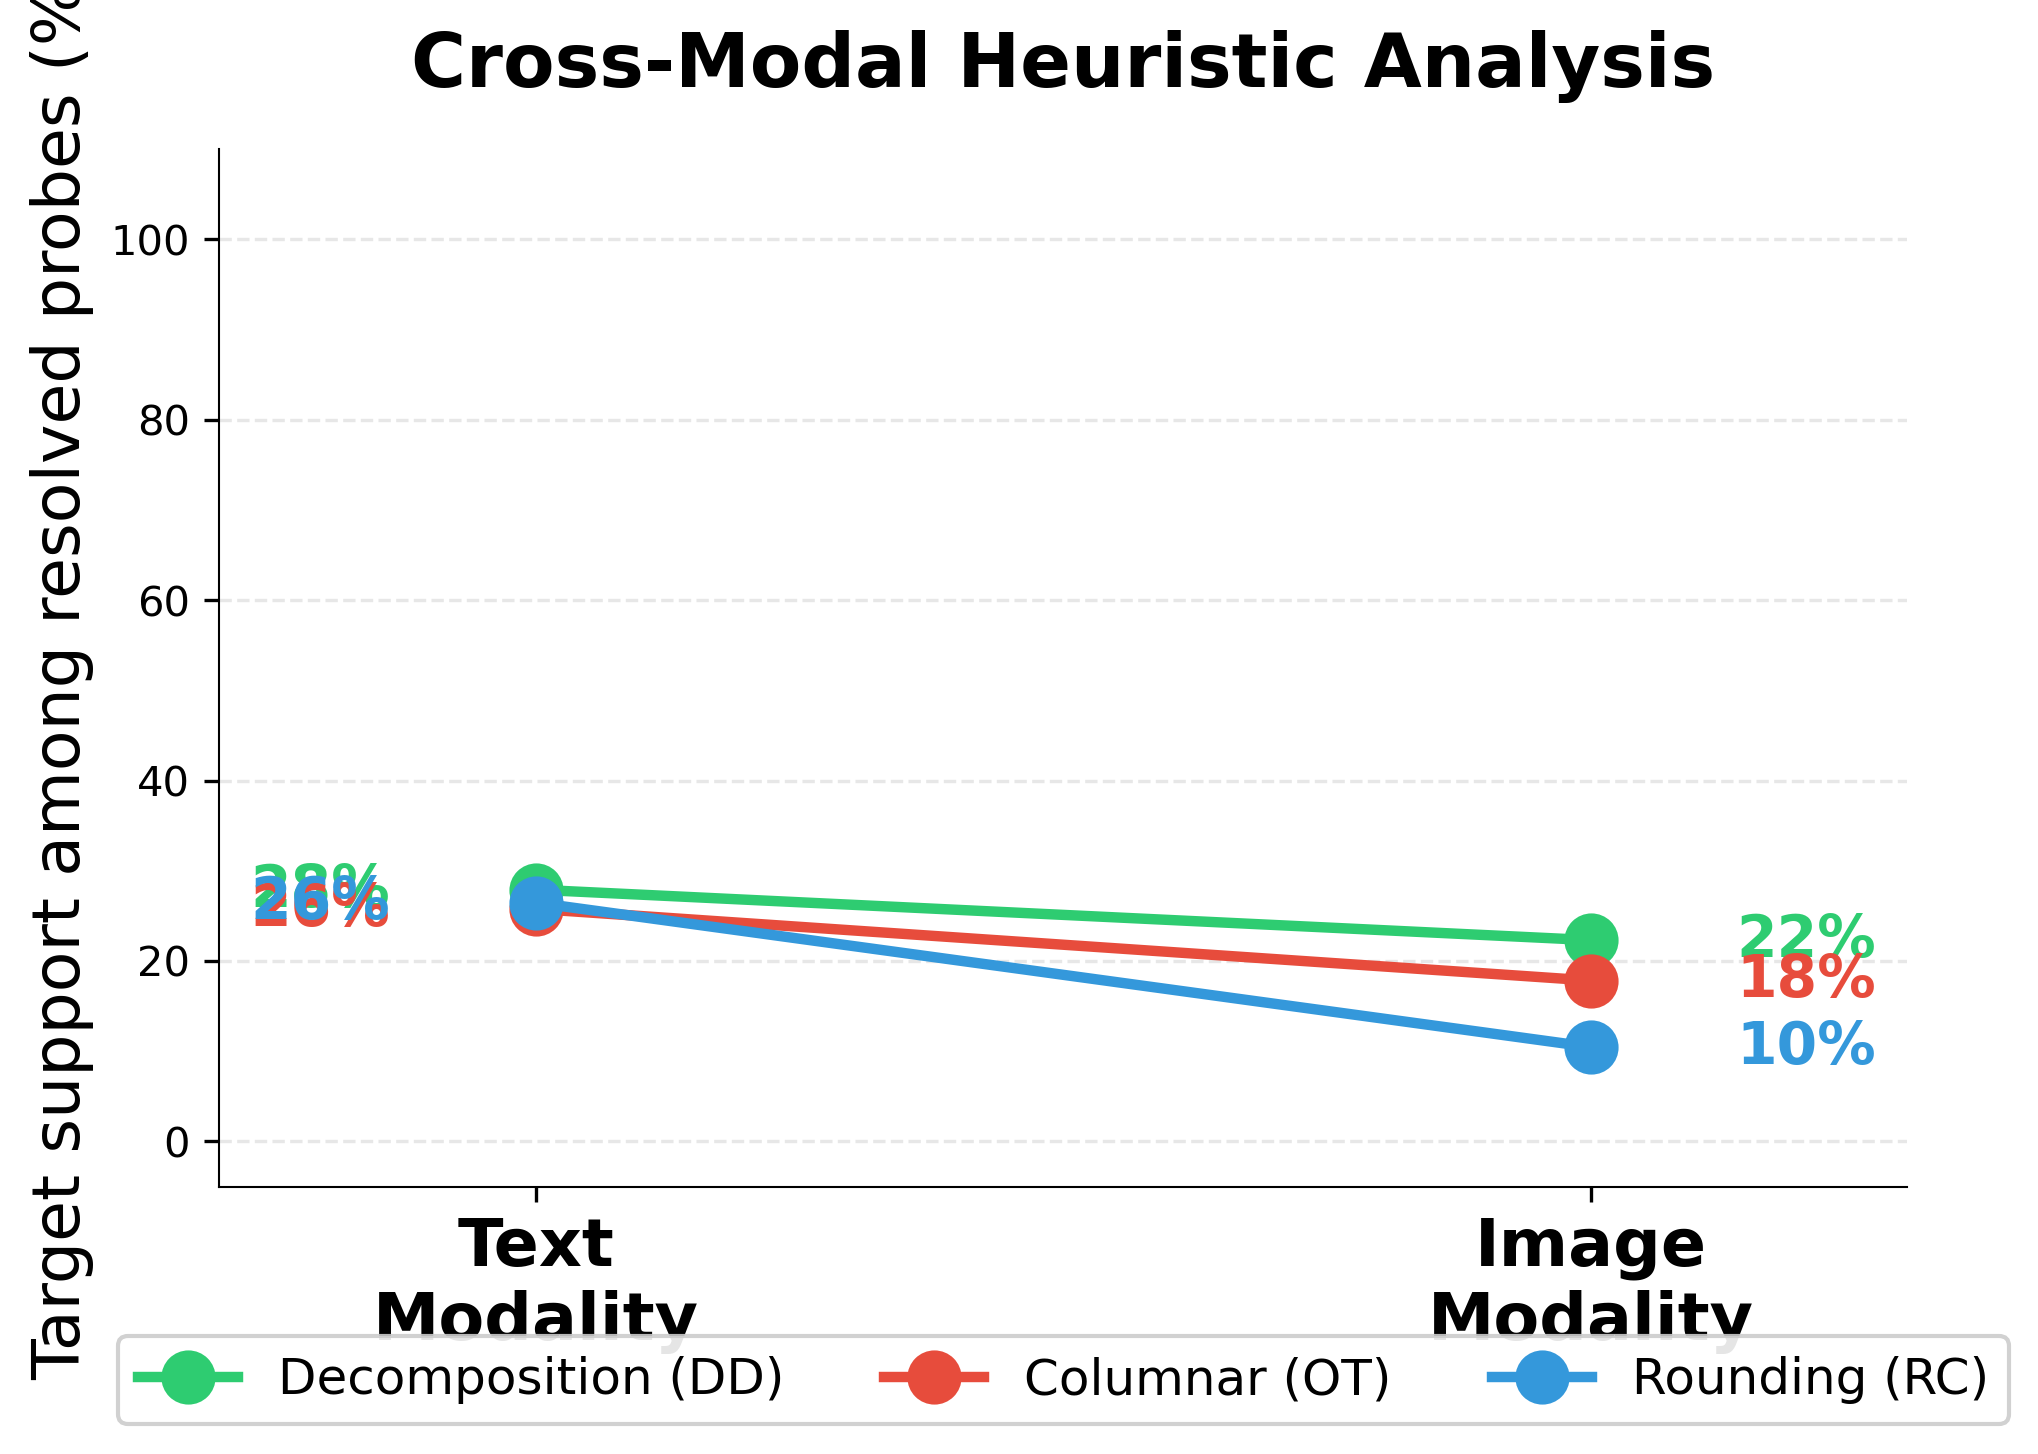
\includegraphics[width=0.85\columnwidth]{Figures/heuristic_reversal.png}
\caption{Cross-Modal Heuristic Analysis. Panels show Qwen3-VL-235B-A22B (left) and Qwen3-VL-30B-A3B (right). Curves report target support among resolved target-type probe items (RC/DD/OT-targeted), where support is the normalized $\exp(-\ell)$ share assigned to the target heuristic against DD/RC/OT/neutral alternatives. The ordering remains model-specific: 30B peaks on RC-targeted items, whereas 235B peaks on DD-targeted items. Coverage is reported separately in Table~\ref{tab:modality-comparison-alt}.}
  \label{fig:reversal}
\end{figure}

\paragraph{Contrastive step probe.} To test method grounding beyond style, we score a correct versus a plausible incorrect intermediate step matched in form for each heuristic (see Table~\ref{tab:contrastive-method}). Most correct-step preferences are at ceiling (100\%) on target-aligned HDS items, so the probe primarily confirms basic grounding. The non-trivial signal comes from the remaining non-ceiling cases: overall preference rates still differ by modality (text overall: \ContrastivePrefRateThirtyB{} / \ContrastivePrefRateTwoThirtyFiveB{}; image overall: \ContrastivePrefRateImageThirtyB{} / \ContrastivePrefRateImageTwoThirtyFiveB{}), with mean loss gaps of \ContrastiveDeltaThirtyB{} / \ContrastiveDeltaTwoThirtyFiveB{} (text) and \ContrastiveDeltaImageThirtyB{} / \ContrastiveDeltaImageTwoThirtyFiveB{} (image). Even at ceiling preference rates, margins vary by heuristic: OT steps show the largest loss gaps while DD is smallest (text OT: \ContrastiveOTDeltaThirtyB{} / \ContrastiveOTDeltaTwoThirtyFiveB{} vs DD: \ContrastiveDDDeltaThirtyB{} / \ContrastiveDDDeltaTwoThirtyFiveB{}; image OT: \ContrastiveOTDeltaImageThirtyB{} / \ContrastiveOTDeltaImageTwoThirtyFiveB{} vs DD: \ContrastiveDDDeltaImageThirtyB{} / \ContrastiveDDDeltaImageTwoThirtyFiveB{}), suggesting the probe reflects step-level constraint strength rather than global heuristic routing, because the contrastive pairs hold surface form fixed and only flip the correctness of a single intermediate step. Table~\ref{tab:contrastive-results} summarizes the contrastive step metrics.

A style-mismatch ablation shows that the loss-based fingerprint is materially more stable than a pure wording-matching account would predict. Overall heuristic-match changes only modestly between balanced and style-mismatch template sets: \TemplateBalancedHeuristicMatchThirtyB{} to \TemplateStyleMismatchHeuristicMatchThirtyB{} in 30B text, \TemplateBalancedHeuristicMatchImageThirtyB{} to \TemplateStyleMismatchHeuristicMatchImageThirtyB{} in 30B image, \TemplateBalancedHeuristicMatchTwoThirtyFiveB{} to \TemplateStyleMismatchHeuristicMatchTwoThirtyFiveB{} in 235B text, and \TemplateBalancedHeuristicMatchImageTwoThirtyFiveB{} to \TemplateStyleMismatchHeuristicMatchImageTwoThirtyFiveB{} in 235B image. Accuracy is likewise stable, with 235B text moving from \TemplateBalancedAccuracyTwoThirtyFiveB{} to \TemplateStyleMismatchAccuracyTwoThirtyFiveB{} and 235B image from \TemplateBalancedAccuracyImageTwoThirtyFiveB{} to \TemplateStyleMismatchAccuracyImageTwoThirtyFiveB{}. Template-level variance remains small in the aggregate as well (balanced/style-mismatch mean within-problem std: \TemplateBalancedMeanStdThirtyB{} / \TemplateStyleMismatchMeanStdThirtyB{} for 30B text, \TemplateBalancedMeanStdImageThirtyB{} / \TemplateStyleMismatchMeanStdImageThirtyB{} for 30B image, \TemplateBalancedMeanStdTwoThirtyFiveB{} / \TemplateStyleMismatchMeanStdTwoThirtyFiveB{} for 235B text, and \TemplateBalancedMeanStdImageTwoThirtyFiveB{} / \TemplateStyleMismatchMeanStdImageTwoThirtyFiveB{} for 235B image; detailed per-heuristic values in Table~\ref{tab:template-variability}). Target-specific shifts remain limited: DD-target detection moves from \TemplateBalancedDDDetectionThirtyB{} to \TemplateStyleMismatchDDDetectionThirtyB{} in 30B text, RC-target detection from \TemplateBalancedRCDetectionImageTwoThirtyFiveB{} to \TemplateStyleMismatchRCDetectionImageTwoThirtyFiveB{} in 235B image, and OT-target detection from \TemplateBalancedOTDetectionImageTwoThirtyFiveB{} to \TemplateStyleMismatchOTDetectionImageTwoThirtyFiveB{} in that same 235B image run. Taken together, these ablations indicate that the cue-conditioned ordering uncovered by the fingerprint is fairly robust to stylistic perturbation, even though some margins do compress under mismatched wording.

\begin{table}[t]
  \centering
  \small
  \begin{tabular}{lp{0.68\columnwidth}}
    \hline
    Element & Description \\
    \hline
    Items & HDS test problems, evaluated with the same $(a,b)$ in text or rendered-image form. \\
    Pair construction & For each heuristic (OT/DD/RC), build a correct step and a plausible incorrect step with identical wording; incorrect numbers are perturbed to nearby values while preserving digit length and trailing-zero structure. \\
    Scoring & Compute forced-completion loss on the step tokens given the same prompt context; lower loss indicates the preferred step. \\
    Metrics & Preference rate (correct loss $<$ incorrect loss) and mean loss gap (incorrect $-$ correct), reported overall and by target heuristic. \\
    \hline
  \end{tabular}
  \caption{Contrastive step probe methodology for text and image inputs.}
  \label{tab:contrastive-method}
\end{table}

These modality differences suggest that the preferred arithmetic heuristic is not solely determined by the mathematical structure of the problem, but also by how the problem is presented. Visual presentation may subtly reweight heuristic margins (e.g., toward rounding-based cues) due to the gestalt perception of number magnitudes in rendered equations \citep{dehaene2011number}. See Appendix for an analysis of heuristics on adversarial traps. 

\subsection{LoRA Nudges Change Behavior, Degrade Performance}

Given that the probes reveal stable heuristic preferences (and that these signals can be stressed under traps), we next ask whether we can \emph{actively} steer strategy selection with lightweight adaptation. We tested whether applying heuristic-specific LoRA adapters could ``nudge'' the model toward different reasoning strategies on held-out problems. Using the Qwen3-VL-30B and Qwen3-VL-235B models (the same models used for fingerprinting), we evaluated on the HDS test split ($n=\NudgeTestCountThirtyB$ / $\NudgeTestCountTwoThirtyFiveB$). Applying the \NudgeLoRACountThirtyB{} / \NudgeLoRACountTwoThirtyFiveB{} trained heuristic LoRAs (RC, DD, OT) produced \NudgeTotalFlipsThirtyB{} / \NudgeTotalFlipsTwoThirtyFiveB{} behavioral (correctness) flips across \NudgeTotalComparisonsThirtyB{} / \NudgeTotalComparisonsTwoThirtyFiveB{} comparisons (\NudgeLoRACountThirtyB{} / \NudgeLoRACountTwoThirtyFiveB{} LoRAs $\times$ \NudgeTestCountThirtyB{} / \NudgeTestCountTwoThirtyFiveB{} problems per model)---\NudgeImprovedThirtyB{} / \NudgeImprovedTwoThirtyFiveB{} improved and \NudgeDegradedThirtyB{} / \NudgeDegradedTwoThirtyFiveB{} degraded---and \NudgeDetectionFlipsThirtyB{} / \NudgeDetectionFlipsTwoThirtyFiveB{} heuristic flips (changes in the lowest-loss template). These headline nudge totals exclude the STYLE control adapter, which we analyze separately below. Degradations dominate improvements for both model sizes, and the post-hoc answer taxonomy shows recurring partial-product omissions, magnitude slips, and carry-drop errors among degraded cases (\NudgeDegradedPartialProductThirtyB{}, \NudgeDegradedMagnitudeSlipThirtyB{}, \NudgeDegradedCarryDropThirtyB{} for 30B; \NudgeDegradedPartialProductTwoThirtyFiveB{}, \NudgeDegradedMagnitudeSlipTwoThirtyFiveB{}, \NudgeDegradedCarryDropTwoThirtyFiveB{} for 235B). These results suggest that while LoRAs successfully learn heuristic-specific reasoning patterns (as evidenced by low validation loss), the model's internal heuristic router is better optimized for performance than any single heuristic; internal preferences appear to handle arithmetic reasoning better than any single enforced trace distribution.

We also evaluate a style-only control adapter, and it strengthens the interpretation of the nudge results as a general trace-steering failure rather than a problem unique to any one arithmetic heuristic. On the HDS test split, the STYLE control yields \StyleControlImprovedThirtyB{} improved cases and \StyleControlDegradedThirtyB{} degraded cases for 30B text, \StyleControlImprovedImageThirtyB{} improved and \StyleControlDegradedImageThirtyB{} degraded for 30B image, \StyleControlImprovedTwoThirtyFiveB{} improved and \StyleControlDegradedTwoThirtyFiveB{} degraded for 235B text, and \StyleControlImprovedImageTwoThirtyFiveB{} improved and \StyleControlDegradedImageTwoThirtyFiveB{} degraded for 235B image. In other words, even an adapter trained to imitate reasoning-trace format without imposing heuristic-specific arithmetic content still reduces correctness much more often than it helps. This suggests that the degradation seen under heuristic LoRAs is not just a consequence of specializing to OT, DD, or RC in particular; more broadly, pushing the model toward a synthetic trace distribution appears to disrupt the base model's native routing over arithmetic behaviors.

\subsubsection{Heuristics Are Orthogonal in Update Space}

Table~\ref{tab:correlation} shows the cosine similarity between the effective LoRA update matrices for the three heuristic adapters. In the full effective-update comparison, adding the STYLE control yields pairwise similarities ranging from \EffectiveUpdateMinCrossThirtyB{} to \EffectiveUpdateMaxCrossThirtyB{} for 30B and from \EffectiveUpdateMinCrossTwoThirtyFiveB{} to \EffectiveUpdateMaxCrossTwoThirtyFiveB{} for 235B, so the 235B adapters are strongly separated while the 30B adapters are only approximately orthogonal. Same-heuristic seeded reruns are more aligned than the primary unseeded cross-heuristic baseline (\EffectiveUpdateSameSeedAvgThirtyB{} vs.\ \EffectiveUpdatePrimaryCrossAvgThirtyB{} with gap \EffectiveUpdateSeedGapThirtyB{} for 30B; \EffectiveUpdateSameSeedAvgTwoThirtyFiveB{} vs.\ \EffectiveUpdatePrimaryCrossAvgTwoThirtyFiveB{} with gap \EffectiveUpdateSeedGapTwoThirtyFiveB{} for 235B), which strengthens the interpretation that the cross-heuristic separation is meaningful rather than incidental.

%To validate that low cosine similarity reflects meaningful separation rather than high-dimensional noise, we train same-heuristic LoRAs with different random seeds. If training is stable, same-heuristic adapters should show higher alignment than cross-heuristic pairs. This control supports that the low-similarity signal is not an artifact of dimensionality.

\section{Discussion}

In sum, our results suggest that multimodal arithmetic brittleness is not merely a matter of ``harder inputs,'' but reflects an interaction between (i)~an algorithmic load that scales predictably with digit structure and (ii)~model-specific procedural priors that are themselves sensitive to representation. Digit complexity provides a compact, mechanistically plausible axis along which accuracy collapses across models and modalities, while forced-completion loss fingerprinting reveals model-specific low-loss preferences rather than a universal decomposition-first bias: 30B is most compatible with RC-like completions, whereas 235B is most compatible with DD-like completions, and image inputs mostly preserve while compressing those margins. The key implication is that ``arithmetic capability'' in modern MM-LLMs is better understood as a mixture of heuristics whose routing is cue- and modality-dependent: rendering the problem as an image or number words can compress heuristic margins, and lightweight specialization can flip the model's preferred continuation without reliably improving correctness.
% Finally, the near-orthogonality of heuristic-specialized LoRA effective updates strengthens the interpretation that these heuristics correspond to separable computational subspaces rather than superficial prompt styles, offering a geometric handle on procedure-level behavior. Together, these findings motivate evaluations (and interventions) that track not only whether a model answers correctly, but which procedure it is likely to invoke under the same arithmetic content presented through different channels.


\section*{Ethics \& Limitations}

Despite the controlled benchmark design and the cross-modal evaluation, our study has several limitations that bound how broadly these findings should be generalized. Our study focuses exclusively on multiplication, so patterns may differ for addition, division, or more complex operations. This scope is compounded by limited model coverage: the multimodal accuracy analyses combine Gemini 2.5 Flash with matched Qwen runs from a companion evaluation pipeline, while the heuristic fingerprinting and LoRA analyses are demonstrated on Qwen3-VL-30B and Qwen3-VL-235B.

Beyond scope and coverage, we rely on synthetic digit templates that may not match real-world mathematical problem distributions. In the same vein, the forced-preamble technique measures template naturalness rather than the model's actual computation path.

Because our heuristic fingerprinting still relies on hand-designed preambles, the measured ``strategy preference'' remains a compatibility signal rather than a direct readout of executed internal algorithms. The released code therefore includes paraphrase ensembles, style-mismatch ablations, and harder contrastive-step controls, but those checks should still be interpreted as robustness probes rather than proof of mechanistic identity.

Finally, this paper combines outputs from two codebases: the companion multimodal evaluation pipeline supplies the end-to-end complexity/regression analyses, while the repository released here supplies the paired benchmark generator plus the Qwen fingerprinting/LoRA experiments. That split improves reproducibility within each layer, but it means readers should interpret the full empirical story as the union of two coordinated pipelines rather than a single monolithic script.

\bibliographystyle{acl_natbib}

% Bibliography entries for the entire Anthology, followed by custom entries
%\bibliography{custom,anthology-overleaf-1,anthology-overleaf-2}

% Custom bibliography entries only
\bibliography{custom}

\appendix

\section{Formal Notes on Operation Counts and Probes}
\label{sec:formal-notes}

\paragraph{Operation-count proxy.} Let $a$ and $b$ have digit lengths $n,m$ and non-zero digit counts $s,t$. Full digit expansion computes exactly $s \cdot t$ non-zero digit products, and at most $s \cdot t - 1$ additions for summing them. A one-sided decomposition that expands the $s$ non-zero digits of $a$ against all $m$ digits of $b$ uses $m \cdot s$ digit multiplications (including by zero digits), of which at most $s \cdot t$ are non-zero; similarly, expanding $b$ against $a$ uses $n \cdot t$. The proxy $C=(n+m)(s+t)$ is monotone in total length and total non-zero digits, and it upper-bounds $m s$ and $n t$ directly and $s t$ up to a factor of 4 (since $s t \le (s+t)^2/4 \le C/4$). It is a coarse proxy and does not, in general, preserve the exact ordering of operation counts.

%\paragraph{Error-rate model.} If each primitive digit operation fails independently with probability $p$, then $P(\text{correct})=(1-p)^{N_{\text{ops}}}$. For small $p$, $P(\text{correct}) \approx \exp(-p N_{\text{ops}})$, implying log-accuracy is linear in $N_{\text{ops}}$. A log link on $P(\text{correct})$ matches this independent-error model; a complementary log-log link would require a different parameterization (e.g., linear in $\log N_{\text{ops}}$) or a hazard-style model. Logistic regression is a convenient monotone fit whose slope should be interpreted as an empirical difficulty parameter rather than a literal per-op error rate.

%\paragraph{Suffix lemma.} In a right-to-left columnar algorithm, the last $k$ output digits depend only on the first $k$ columns of computation. Let $E_k$ be the event that all of the first $k$ columns are correct; then $\Pr[\text{last $k$ digits correct}] \ge \Pr[E_k]$. This is an unconditional bound; the conditional metric we plot, $\Pr[\text{last $k$ digits correct} \mid \text{wrong}]$, can differ without assumptions on error distribution. Under a simple independent per-column error model with per-column correctness $q$ across $L$ columns, for example,
%\[\Pr[\text{last digit correct} \mid \text{wrong}] = \frac{q(1-q^{L-1})}{1-q^L},\]
%which remains well above the naive $1/10$ reference unless $q$ is near chance. We therefore interpret conditional suffix accuracy that falls below columnar expectations as evidence against dominant columnar computation only under such error-spread assumptions.

\paragraph{Heuristic cost models.} We assign each heuristic a cost proxy based on primitive digit operations: OT uses the schoolbook cost $n \cdot m$ digit multiplications plus a small carry/accumulation penalty; DD uses one-sided expansion cost $\min(m \cdot s, n \cdot t)$ plus additions for combining partial products, with explicit low-cost special cases for trailing-zero and quarter-hundred factors; RC uses a shared-base correction cost built from the nearest round base and the two operand offsets. In the current HDSv2 release these cost models are the canonical labeling rule, and items are retained only when the minimum-cost heuristic is uniquely separated from the runner-up by a fixed margin.

\paragraph{HDS construction.} We seed the Heuristic-Disagreement Set (HDS) with a hand-curated pool of problems that exemplify each heuristic: RC problems sit near round bases (e.g., 50, 100, 200), DD problems have trailing zeros or clean factors (e.g., $\times 10$, $\times 25$), and OT problems are deliberately unstructured or carry-heavy. We also include small perturbation pairs that flip a single cue (near-base vs.\ not, zero vs.\ not) to test causal sensitivity of heuristic detection. Curated problems that disagree with the cost-model winner are audited rather than force-labeled into the canonical dataset.

We then scale to a target count by sampling additional items in three buckets, allocating roughly equal quotas per design family: RC draws offsets within $\pm 10$ around bases \{25, 50, 100, 200, 250, 500\}; DD draws problems with trailing zeros, multiples of 25, or clean tens decompositions; OT draws carry-heavy high-digit pairs or generic pairs explicitly away from near-base and zero cues. We enforce uniqueness up to commutativity, generate traps disjoint from HDS, and stratify train/val/test splits by canonical target heuristic using \DatasetSplitRatios{} to preserve the intended mix across splits.

\paragraph{Likelihood-ratio probe.} Let $x_h$ be the heuristic template tokens and $\ell(h)=-\frac{1}{T_h}\sum_{t=1}^{T_h} \log p(x_{h,t}\mid c)$ the length-normalized cross-entropy under the same base model for context $c$ (the multiplication problem), computed on forced continuation tokens. If templates are token-length matched ($T_h=T$), then $-T \Delta \ell(h)$ equals the log-likelihood ratio $\log \frac{p(x_h\mid c)}{p(x_0\mid c)}$ between candidate templates under the same model. Selecting the minimum-loss heuristic is therefore the maximum-likelihood choice among candidates under equal priors; when token lengths differ, $\Delta \ell$ is a normalized naturalness score rather than an exact ML decision rule.

\section{Supplementary Complexity Fits}
\label{sec:complexity-fits}

We provide additional regression fits for Qwen3-VL-30B and Qwen3-VL-235B on the numerical-text and numerical-image modalities (no audio) in Tables~\ref{tab:regression-text} and \ref{tab:regression-image}, reporting linear probability model regression coefficients for total digits, total non-zero digits, and their product in the numerical-text and numerical-image conditions.

\begin{table*}[t]
\centering
\caption{Linear probability model coefficients predicting probability of a correct answer from input features for numeric-text prompts. Standard errors are in parentheses; * indicates $p<0.05$.}
\label{tab:regression-text}
\resizebox{\textwidth}{!}{%
\begin{tabular}{lccc}
\toprule
 & google-gemini-2.5-flash & qwen-qwen3-vl-235b-a22b-instruct & qwen-qwen3-vl-30b-a3b-instruct \\
%Feature &  &  &  \\
\midrule
\textit{Intercept} & 1.431*
(0.067) & 0.649*
(0.067) & 1.420*
(0.066) \\
\textit{Total digits} & -0.001
(0.008) & 0.087*
(0.008) & -0.005
(0.008) \\
\textit{Total non-zero digits} & -0.170*
(0.017) & 0.107*
(0.018) & -0.154*
(0.017) \\
\textit{Digit complexity} & 0.002
(0.002) & -0.025*
(0.002) & 0.001
(0.002) \\
\bottomrule
\end{tabular}
}
\end{table*}

\begin{table*}[t]
\centering
\caption{Linear probability model coefficients predicting probability of a correct answer from input features for numeric-image prompts. Standard errors are in parentheses; * indicates $p<0.05$.}
\label{tab:regression-image}
\resizebox{\textwidth}{!}{%
\begin{tabular}{lccc}
\toprule
 & google-gemini-2.5-flash & qwen-qwen3-vl-235b-a22b-instruct & qwen-qwen3-vl-30b-a3b-instruct \\
%Feature &  &  &  \\
\midrule
\textit{Intercept} & 1.418*
(0.066) & 1.175*
(0.073) & 1.406*
(0.065) \\
\textit{Total digits} & -0.005
(0.008) & 0.009
(0.009) & -0.003
(0.008) \\
\textit{Total non-zero digits} & -0.152*
(0.017) & -0.032
(0.019) & -0.149*
(0.017) \\
\textit{Digit complexity} & 0.001
(0.002) & -0.010*
(0.002) & 0.000
(0.002) \\
\bottomrule
\end{tabular}
}
\end{table*}


\section{Forced-Completion Loss Probe Templates}
\label{sec:templates}

Our forced-completion loss probe uses heuristic-specific assistant continuations designed to be short and style-matched. The default balanced template bank contains multiple paraphrases per heuristic; below we show one representative continuation for each class:

\paragraph{Columnar (OT)}
\begin{quote}
``Column method: start with the ones digits''
\end{quote}

\paragraph{Decomposition (DD)}
\begin{quote}
``Decomposition: split one factor into place-value parts''
\end{quote}

\paragraph{Rounding-Compensation (RC)}
\begin{quote}
``Round and adjust: use a nearby round base, then compensate''
\end{quote}

\paragraph{Neutral Baseline}
\begin{quote}
``Let me solve this multiplication problem step by step''
\end{quote}

We compute cross-entropy loss over the template continuation tokens (masking constant wrappers) under forced completion and report the difference ($\Delta$loss) relative to the neutral baseline. The active bank is intentionally short and stylistically matched but not strictly token-length identical, so we use length-normalized loss to mitigate residual token-length differences.

\section{Evaluation Protocol}
\label{sec:protocol}

\paragraph{Decoding Parameters} All generations in the released Qwen probing/LoRA pipeline use temperature $= 0$ (deterministic). The current default maximum generation budget is 2048 tokens for both direct-answer and reasoning-enabled calls unless explicitly overridden by script arguments.

\paragraph{Uncertainty Estimates} Standard errors (±SE) are computed across problem instances. For accuracy and resolved-probe coverage we use the binomial SE $\sqrt{p(1-p)/n}$ (reported in percentage points). For loss averages and resolved-probe target support we use the sample standard deviation of per-problem values divided by $\sqrt{n}$, with target-support SE computed only across the resolved rows for that family. With deterministic decoding (temperature $=0$), these SEs reflect item-level variability rather than sampling noise.

\paragraph{Answer Parsing} For the released Qwen probing/LoRA pipeline, we use an enhanced priority-ordered answer extractor rather than a single last-integer regex rule. The parser checks boxed/final-answer/equation-style markers before falling back to later numeric candidates, validates extracted answers against the expected operand scale when operands are provided, and records extraction metadata including confidence, truncation status, and contamination flags when a trace appears to solve the wrong problem.

\section{Raw Forced-Completion Loss Results}
\label{sec:raw-loss}

For completeness, we report raw cross-entropy losses (with SE) under forced completion and the original modality comparison table. These absolute losses underlie the $\Delta$loss summaries in the main text.

\begin{table}[t]
  \centering
  \begin{tabular}{lc}
    \hline
    Heuristic & 30B/235B Avg. Loss $\pm$ SE \\
    \hline
    DD (Decomposition) & \HDSTestPerpDDThirtyB{} $\pm$ \HDSTestPerpDDSEThirtyB{} / \HDSTestPerpDDTwoThirtyFiveB{} $\pm$ \HDSTestPerpDDSETwoThirtyFiveB{} \\
    RC (Rounding) & \HDSTestPerpRCThirtyB{} $\pm$ \HDSTestPerpRCSEThirtyB{} / \HDSTestPerpRCTwoThirtyFiveB{} $\pm$ \HDSTestPerpRCSETwoThirtyFiveB{} \\
    OT (Columnar) & \HDSTestPerpOTThirtyB{} $\pm$ \HDSTestPerpOTSEThirtyB{} / \HDSTestPerpOTTwoThirtyFiveB{} $\pm$ \HDSTestPerpOTSETwoThirtyFiveB{} \\
    \hline
  \end{tabular}
  \caption{Raw cross-entropy loss by heuristic template on the held-out probe split ($n=\HDSProbeCount$). Lower values indicate lower forced-completion loss (a deeper continuation preference). In the canonical probe runs, RC has the lowest raw loss for 30B while DD has the lowest raw loss for 235B, so the low-loss ordering is model-specific rather than uniformly decomposition-first.}
  \label{tab:loss-raw}
\end{table}

\begin{figure}[t]
  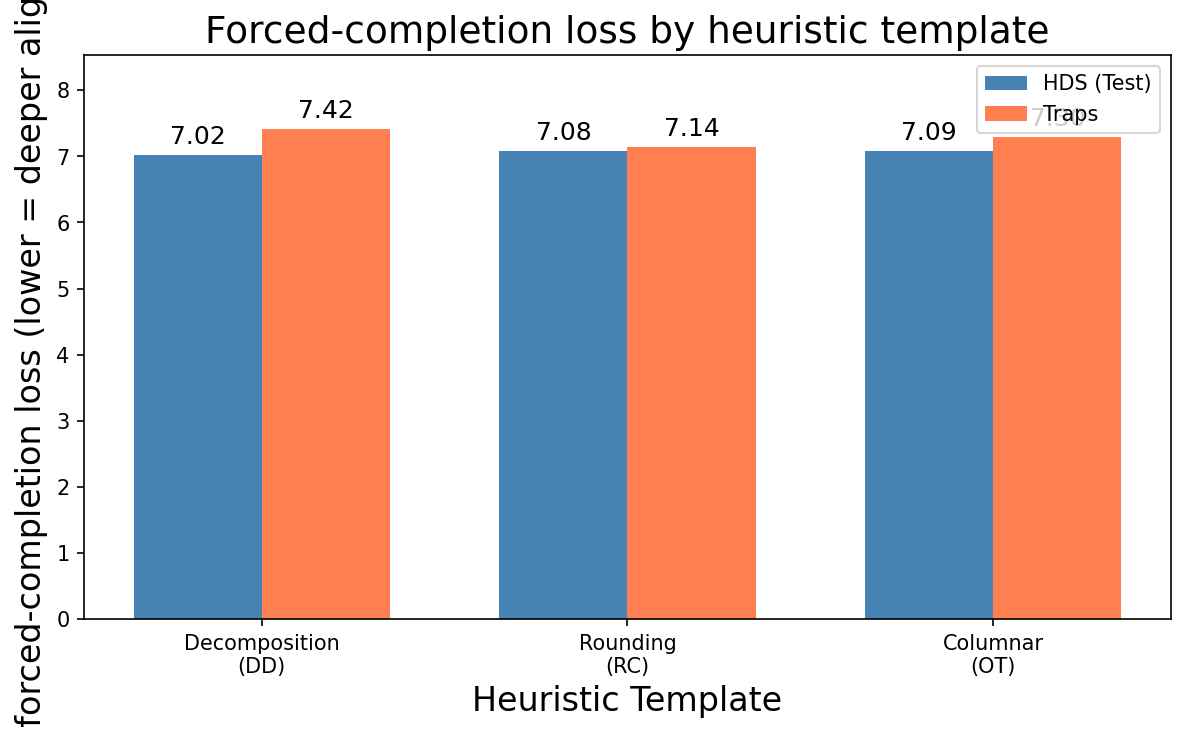
\includegraphics[width=\columnwidth]{Figures/perplexity_comparison.png}
  \caption{Raw cross-entropy loss by heuristic template on the held-out probe split and adversarial Traps datasets. Panels show Qwen3-VL-30B (left) and Qwen3-VL-235B (right). The lowest-loss heuristic is model-specific rather than uniformly DD-first: on the probe split, RC is lowest for Qwen3-VL-30B while DD is lowest for Qwen3-VL-235B (Table~\ref{tab:loss-raw}).}
  \label{fig:loss-comparison-raw}
\end{figure}

\begin{comment}
\begin{table*}[t]
  \centering
  \begin{tabular}{llcc}
    \hline
    \textbf{Metric} & \textbf{Model} & \textbf{Text} & \textbf{Image} \\
    \hline
    \HDSProbeAccuracyMeanCLabel{} & 30B & \HDSTestAccuracyThirtyB{} $\pm$ \HDSTestAccuracySEThirtyB{} & \HDSTestAccuracyImageThirtyB{} $\pm$ \HDSTestAccuracyImageSEThirtyB{} \\
    & 235B & \HDSTestAccuracyTwoThirtyFiveB{} $\pm$ \HDSTestAccuracySETwoThirtyFiveB{} & \HDSTestAccuracyImageTwoThirtyFiveB{} $\pm$ \HDSTestAccuracyImageSETwoThirtyFiveB{} \\
    \hline
    \multicolumn{4}{l}{\textit{Cross-entropy loss (lower = deeper alignment):}} \\
    \quad DD (Decomposition) & 30B & \HDSTestPerpDDThirtyB{} $\pm$ \HDSTestPerpDDSEThirtyB{} & \HDSTestPerpDDImageThirtyB{} $\pm$ \HDSTestPerpDDImageSEThirtyB{} \\
    & 235B & \HDSTestPerpDDTwoThirtyFiveB{} $\pm$ \HDSTestPerpDDSETwoThirtyFiveB{} & \HDSTestPerpDDImageTwoThirtyFiveB{} $\pm$ \HDSTestPerpDDImageSETwoThirtyFiveB{} \\
    \quad RC (Rounding) & 30B & \HDSTestPerpRCThirtyB{} $\pm$ \HDSTestPerpRCSEThirtyB{} & \HDSTestPerpRCImageThirtyB{} $\pm$ \HDSTestPerpRCImageSEThirtyB{} \\
    & 235B & \HDSTestPerpRCTwoThirtyFiveB{} $\pm$ \HDSTestPerpRCSETwoThirtyFiveB{} & \HDSTestPerpRCImageTwoThirtyFiveB{} $\pm$ \HDSTestPerpRCImageSETwoThirtyFiveB{} \\
    \quad OT (Columnar) & 30B & \HDSTestPerpOTThirtyB{} $\pm$ \HDSTestPerpOTSEThirtyB{} & \HDSTestPerpOTImageThirtyB{} $\pm$ \HDSTestPerpOTImageSEThirtyB{} \\
    & 235B & \HDSTestPerpOTTwoThirtyFiveB{} $\pm$ \HDSTestPerpOTSETwoThirtyFiveB{} & \HDSTestPerpOTImageTwoThirtyFiveB{} $\pm$ \HDSTestPerpOTImageSETwoThirtyFiveB{} \\
    \hline
    \multicolumn{4}{l}{\textit{Lowest-loss match rate on target problems:}} \\
    \quad DD match (on DD-targeted items) & 30B & \HDSTestDDDetectionThirtyB{} $\pm$ \HDSTestDDDetectionSEThirtyB{} & \HDSTestDDDetectionImageThirtyB{} $\pm$ \HDSTestDDDetectionImageSEThirtyB{} \\
    & 235B & \HDSTestDDDetectionTwoThirtyFiveB{} $\pm$ \HDSTestDDDetectionSETwoThirtyFiveB{} & \HDSTestDDDetectionImageTwoThirtyFiveB{} $\pm$ \HDSTestDDDetectionImageSETwoThirtyFiveB{} \\
    \quad RC match (on RC-targeted items) & 30B & \HDSTestRCDetectionThirtyB{} $\pm$ \HDSTestRCDetectionSEThirtyB{} & \HDSTestRCDetectionImageThirtyB{} $\pm$ \HDSTestRCDetectionImageSEThirtyB{} \\
    & 235B & \HDSTestRCDetectionTwoThirtyFiveB{} $\pm$ \HDSTestRCDetectionSETwoThirtyFiveB{} & \HDSTestRCDetectionImageTwoThirtyFiveB{} $\pm$ \HDSTestRCDetectionImageSETwoThirtyFiveB{} \\
    \quad OT match (on OT-targeted items) & 30B & \HDSTestOTDetectionThirtyB{} $\pm$ \HDSTestOTDetectionSEThirtyB{} & \HDSTestOTDetectionImageThirtyB{} $\pm$ \HDSTestOTDetectionImageSEThirtyB{} \\
    & 235B & \HDSTestOTDetectionTwoThirtyFiveB{} $\pm$ \HDSTestOTDetectionSETwoThirtyFiveB{} & \HDSTestOTDetectionImageTwoThirtyFiveB{} $\pm$ \HDSTestOTDetectionImageSETwoThirtyFiveB{} \\
    \hline
  \end{tabular}
  \caption{Modality comparison on a shared held-out probe split ($n=\HDSProbeCount$) for Qwen3-VL-30B and Qwen3-VL-235B using raw cross-entropy losses. Lowest-loss match rate is computed on probe items designed to favor each heuristic (e.g., near-base pairs for RC, trailing zeros or clean decompositions for DD, carry-heavy digit pairs for OT) and reports the share where that heuristic attains the lowest forced-completion loss.}
  \label{tab:modality-comparison-raw}
\end{table*}
\end{comment}

\section{Embedding-Based Trace Fingerprint}
\label{sec:embedding-fingerprint}

% Auto-generated merged embedding fingerprint appendix
% Generated by Scripts/analysis/GenerateResultsFigures.py

\paragraph{Embedding-based trace summary.} Prototype-embedding trace summaries are currently available only for the image fingerprint runs in the canonical artifacts. 30B: DD/OT contribute \HDSTestTraceEmbedDDCountImageThirtyB{} / \HDSTestTraceEmbedOTCountImageThirtyB{} of \HDSTestTraceEmbedResolvedTotalImageThirtyB{} resolved traces, with RC/STYLE at \HDSTestTraceEmbedRCCountImageThirtyB{} / \HDSTestTraceEmbedSTYLECountImageThirtyB{}; 235B: DD/OT contribute \HDSTestTraceEmbedDDCountImageTwoThirtyFiveB{} / \HDSTestTraceEmbedOTCountImageTwoThirtyFiveB{} of \HDSTestTraceEmbedResolvedTotalImageTwoThirtyFiveB{} resolved traces, with RC/STYLE at \HDSTestTraceEmbedRCCountImageTwoThirtyFiveB{} / \HDSTestTraceEmbedSTYLECountImageTwoThirtyFiveB{}.
Across target-labeled image items, DD and OT remain stronger than RC in the embedding-based detector (30B: DD \HDSTestDDTraceEmbedDetectionImageAltThirtyB{}, OT \HDSTestOTTraceEmbedDetectionImageAltThirtyB{}, RC \HDSTestRCTraceEmbedDetectionImageAltThirtyB{}; 235B: DD \HDSTestDDTraceEmbedDetectionImageAltTwoThirtyFiveB{}, OT \HDSTestOTTraceEmbedDetectionImageAltTwoThirtyFiveB{}, RC \HDSTestRCTraceEmbedDetectionImageAltTwoThirtyFiveB{}).

\begin{table}[htbp]
\centering
\caption{Embedding-based trace fingerprint summary by model (prototype classifier, image modality only)}
\label{tab:embedding-fingerprint}
\begin{tabular}{@{}lccc@{}}
\toprule
Slice & Coverage & Target support & Detection \\
\midrule
\multicolumn{4}{@{}l@{}}{\textbf{30B}} \\
All image traces resolved & \HDSTestResolvedTraceEmbedCoverageImageAltThirtyB{} & N/A & N/A \\
DD-targeted items & \HDSTestDDTraceEmbedCoverageImageAltThirtyB{} & \HDSTestDDTraceEmbedTargetSupportImageAltThirtyB{} & \HDSTestDDTraceEmbedDetectionImageAltThirtyB{} \\
OT-targeted items & \HDSTestOTTraceEmbedCoverageImageAltThirtyB{} & \HDSTestOTTraceEmbedTargetSupportImageAltThirtyB{} & \HDSTestOTTraceEmbedDetectionImageAltThirtyB{} \\
RC-targeted items & \HDSTestRCTraceEmbedCoverageImageAltThirtyB{} & \HDSTestRCTraceEmbedTargetSupportImageAltThirtyB{} & \HDSTestRCTraceEmbedDetectionImageAltThirtyB{} \\
\midrule
\multicolumn{4}{@{}l@{}}{\textbf{235B}} \\
All image traces resolved & \HDSTestResolvedTraceEmbedCoverageImageAltTwoThirtyFiveB{} & N/A & N/A \\
DD-targeted items & \HDSTestDDTraceEmbedCoverageImageAltTwoThirtyFiveB{} & \HDSTestDDTraceEmbedTargetSupportImageAltTwoThirtyFiveB{} & \HDSTestDDTraceEmbedDetectionImageAltTwoThirtyFiveB{} \\
OT-targeted items & \HDSTestOTTraceEmbedCoverageImageAltTwoThirtyFiveB{} & \HDSTestOTTraceEmbedTargetSupportImageAltTwoThirtyFiveB{} & \HDSTestOTTraceEmbedDetectionImageAltTwoThirtyFiveB{} \\
RC-targeted items & \HDSTestRCTraceEmbedCoverageImageAltTwoThirtyFiveB{} & \HDSTestRCTraceEmbedTargetSupportImageAltTwoThirtyFiveB{} & \HDSTestRCTraceEmbedDetectionImageAltTwoThirtyFiveB{} \\
\bottomrule
\end{tabular}
\end{table}


\section{Fingerprinting Examples}
\label{sec:fingerprint-examples}

Table~\ref{tab:fingerprint-examples} shows representative examples from our heuristic fingerprinting experiments on the HDS test split, comparing text and image modality results on identical problems. Each row shows a multiplication problem, its target heuristic, and the lowest-loss heuristic with confidence for both text and image inputs. The table illustrates modality-dependent differences in lowest-loss heuristic labels on a subset of problems, consistent with cue-driven reweighting rather than a wholesale switch. This modality gap suggests that the model's arithmetic strategy selection depends on input representation, not just problem structure.

% Auto-generated fingerprint examples (text vs image comparison)
% Generated by Scripts/analysis/GenerateResultsFigures.py

\begin{table}[htbp]
\centering
\caption{Example Fingerprinting Results (lowest-loss heuristic): Text vs Image Modality}
\label{tab:fingerprint-examples}
\small
\begin{tabular}{@{}lccccc@{}}
\toprule
Problem & Target & \multicolumn{2}{c}{Text} & \multicolumn{2}{c}{Image} \\
\cmidrule(lr){3-4} \cmidrule(lr){5-6}
        &        & Lowest-loss & Conf & Lowest-loss & Conf \\
\midrule
$453 \times 900$ & DD & DD & 0.00 & RC & 0.01 \\
$43 \times 67$ & OT & DD & 0.08 & DD & 0.09 \\
$96 \times 98$ & RC & DD & 0.18 & DD & 0.19 \\
$28 \times 28$ & RC & DD & 0.18 & DD & 0.18 \\
$200 \times 300$ & DD & DD & 0.10 & DD & 0.10 \\
\bottomrule
\end{tabular}
\end{table}


\section{LoRA Training Examples}
\label{sec:training-examples}

We trained heuristic-specific LoRA adapters using synthetic reasoning traces. Below are representative examples showing the expected reasoning pattern for each heuristic. These traces were generated programmatically to ensure consistent structure while varying the specific numbers.

\paragraph{Trace Generation}
Each heuristic uses a distinct algorithmic template:
\begin{itemize}
    \item \textbf{RC}: For symmetric pairs ($a = \text{base} + k$, $b = \text{base} - k$), applies the difference of squares identity $(a)(b) = \text{base}^2 - k^2$. Non-symmetric pairs use a general rounding approach with four adjustment terms.
    \item \textbf{DD}: Decomposes the larger operand into tens and ones components, computes two partial products via the distributive property, and sums them.
    \item \textbf{OT}: Simulates columnar multiplication with explicit digit-by-digit products, carries, and partial product accumulation.
\end{itemize}

\paragraph{Problem Selection}
Problems were selected to match each heuristic's strengths, using the actual programmatic generators released with the repository. RC examples draw from bases \{25, 50, 75, 100, 125, 150, 175, 200, 250, 300, 400, 500\} with offsets 1--5, including both symmetric and mixed near-base pairs. DD examples mix trailing-zero factors, easy tens-plus-ones decompositions, and generic two-digit pairs. OT examples mix carry-heavy 2--3 digit pairs with generic multi-digit numbers. The released generator also supports a STYLE control dataset with generic trace formatting but no heuristic-specific intermediate computation.

\paragraph{Data Leakage Prevention}
To ensure unbiased evaluation, we exclude all HDS validation/test problems, Traps problems, and held-out multimodal problems from training data using commutative problem fingerprints. Concretely, each multiplication instance is keyed as \texttt{min(a,b):max(a,b)}, so $(a,b)$ and $(b,a)$ are treated as the same example for leakage checks.

% Auto-generated LoRA training examples
% Generated by Scripts/analysis/GenerateResultsFigures.py

% Requires: \usepackage{listings} in preamble

\subsection*{Rounding-Compensation (RC) Example}
Problem: $399 \times 399 = 159201$

\begin{lstlisting}[basicstyle=\small\ttfamily,breaklines=true,literate={×}{{$\times$}}1 {²}{{$^2$}}1]
What is 399 × 399?
Let me round to convenient bases and adjust.
399 is close to 400 (difference: -1).
399 is close to 400 (difference: -1).
Start with 400 × 400 = 160000.
Adjustment for 399: 400 × -1 = -400.
Adjustment for 399: -1 × 400 = -400.
Cross term: -1 × -1 = +1.
Total: 160000 + (-400) + (-400) + (+1) = 159201.
Answer: 159201
\end{lstlisting}

\subsection*{Decomposition (DD) Example}
Problem: $99 \times 40 = 3960$

\begin{lstlisting}[basicstyle=\small\ttfamily,breaklines=true,literate={×}{{$\times$}}1 {²}{{$^2$}}1]
What is 99 × 40?
Let me decompose 99 into 90 + 9.
First compute 90 × 40:
90 × 40 = 3600.
Then compute 9 × 40:
9 × 40 = 360.
Now sum the partial products:
3600 + 360 = 3960.
Answer: 3960
\end{lstlisting}

\subsection*{Ones-Then-Tens (OT) Example}
Problem: $79 \times 78 = 6162$

\begin{lstlisting}[basicstyle=\small\ttfamily,breaklines=true,literate={×}{{$\times$}}1 {²}{{$^2$}}1]
What is 79 × 78?
Let me use column multiplication step by step.
Step 1: Multiply 79 by ones digit 8:
  9 × 8 = 72, write 2, carry 7.
  7 × 8 = 56, plus carry = 63.
  First partial product: 632.
Step 2: Multiply 79 by tens digit 7:
  9 × 7 = 63, write 3, carry 6.
  7 × 7 = 49, plus carry = 55.
  Second partial product: 553 (shifted by 10 = 5530).
Step 3: Add partial products:
  632 + 5530 = 6162.
Answer: 6162
\end{lstlisting}


\section{LoRA Nudge Test Examples}
\label{sec:nudge-examples}

Table~\ref{tab:nudge-examples} compares base model behavior across text and image modalities, including LoRA adapter effects for text inputs. Each cell shows correctness (\checkmark/\texttimes) and the lowest-loss heuristic label; correctness flips correspond to changes in the checkmark state, while detection flips correspond to changes in the parenthetical heuristic label. Image modality detection shows the same modality-dependent shifts seen in fingerprinting, demonstrating that both the decomposition prior and the modality gap are deeply embedded.

% Auto-generated merged nudge test examples (text vs image)
% Generated by Scripts/analysis/GenerateResultsFigures.py

\begin{table}[htbp]
\centering
\caption{LoRA Nudge Test Examples by Model: Text vs Image Modality (lowest-loss heuristic)}
\label{tab:nudge-examples}
\begin{tabular}{@{}lccccc@{}}
\toprule
Problem & Target & \multicolumn{2}{c}{Text} & \multicolumn{2}{c}{Image} \\
\cmidrule(lr){3-4} \cmidrule(lr){5-6}
        &        & Base & LoRA & Base & LoRA \\
\midrule
\multicolumn{6}{@{}l@{}}{\textbf{30B}} \\
$901 \times 1055$ & RC & \checkmark (RC) & \checkmark (OT) & \checkmark (OT) & \checkmark (OT) \\
$900 \times 2400$ & DD & \checkmark (RC) & \checkmark (OT) & \checkmark (OT) & \checkmark (OT) \\
$59 \times 38$ & OT & \checkmark (RC) & \checkmark (OT) & \checkmark (DD) & \checkmark (OT) \\
$902 \times 1700$ & DD & \checkmark (RC) & \texttimes (OT) & \checkmark (OT) & \texttimes (OT) \\
$62294 \times 50$ & DD & \checkmark (RC) & \texttimes (OT) & \checkmark (OT) & \texttimes (OT) \\
\midrule
\multicolumn{6}{@{}l@{}}{\textbf{235B}} \\
$901 \times 1055$ & RC & \checkmark (DD) & \checkmark (OT) & \checkmark (DD) & ? (OT) \\
$900 \times 2400$ & DD & \checkmark (DD) & \checkmark (OT) & \checkmark (DD) & \checkmark (OT) \\
$59 \times 38$ & OT & \checkmark (DD) & \checkmark (OT) & \checkmark (DD) & \checkmark (OT) \\
$902 \times 1700$ & DD & \checkmark (DD) & \checkmark (OT) & \checkmark (DD) & \checkmark (OT) \\
$62294 \times 50$ & DD & \checkmark (RC) & \checkmark (OT) & \checkmark (DD) & \checkmark (OT) \\
\bottomrule
\end{tabular}
\end{table}


\section{Adapter Weight Similarity}
\label{sec:similarity}

Table~\ref{tab:similarity-matrix} shows the cosine similarity between flattened LoRA factor weights (A/B), concatenated across all LoRA modules. Because the factorization is not unique, these weight-space cosines are parameterization-dependent; we report them as a supplementary reference alongside the gauge-invariant effective-update similarities in the main text.

% Auto-generated merged cosine similarity matrix
% Generated by Scripts/analysis/GenerateResultsFigures.py

\begin{table}[htbp]
\centering
\caption{Adapter Weight Cosine Similarity Matrix by model (cosine over concatenated flattened LoRA A/B factors across all modules)}
\label{tab:similarity-matrix}
\begin{tabular}{@{}lccc@{}}
\toprule
 & DD & OT & RC \\
\midrule
\multicolumn{4}{@{}l@{}}{\textbf{30B}} \\
DD & 1.0000 & -0.0193 & 0.0365 \\
OT & -0.0193 & 1.0000 & 0.0056 \\
RC & 0.0365 & 0.0056 & 1.0000 \\
\midrule
\multicolumn{4}{@{}l@{}}{\textbf{235B}} \\
DD & 1.0000 & 0.0012 & 0.0022 \\
OT & 0.0012 & 1.0000 & -0.0023 \\
RC & 0.0022 & -0.0023 & 1.0000 \\
\bottomrule
\end{tabular}
\end{table}
% 30B average off-diagonal similarity: 0.0076
% 235B average off-diagonal similarity: 0.0004
% Values near 0 indicate orthogonal (independent) adapter directions
\begin{table}[htbp]
\centering
\caption{Effective-Update Seed-Control Summary by model (same-heuristic unseeded vs seeded controls compared against primary unseeded cross-heuristic pairs)}
\label{tab:similarity-seed-controls}
\begin{tabular}{@{}lc@{}}
\toprule
Pair & Cosine \\
\midrule
\multicolumn{2}{@{}l@{}}{\textbf{30B}} \\
DD-DD seed 123 & 0.2358 \\
OT-OT seed 123 & 0.1640 \\
RC-RC seed 123 & 0.3660 \\
\midrule
Same-heuristic average & 0.2553 \\
Primary cross-heuristic average & 0.1055 \\
Gap & 0.1498 \\
\midrule
\multicolumn{2}{@{}l@{}}{\textbf{235B}} \\
DD-DD seed 123 & 0.1112 \\
OT-OT seed 123 & 0.1633 \\
RC-RC seed 123 & 0.1683 \\
\midrule
Same-heuristic average & 0.1476 \\
Primary cross-heuristic average & 0.0447 \\
Gap & 0.1029 \\
\bottomrule
\end{tabular}
\end{table}
% 30B primary cross-heuristic baseline pairs: DD-OT=0.0726, DD-RC=0.1192, OT-RC=0.1247
% 235B primary cross-heuristic baseline pairs: DD-OT=0.0412, DD-RC=0.0342, OT-RC=0.0586

% Auto-generated merged template-variability appendix
% Generated by Scripts/analysis/GenerateResultsFigures.py

\begin{table}[htbp]
\centering
\caption{Template-variability robustness summary by model (mean within-problem standard deviation across paraphrase losses)}
\label{tab:template-variability}
\begin{tabular}{@{}lcccc@{}}
\toprule
Profile & DD std & OT std & RC std & Mean std \\
\midrule
\multicolumn{5}{@{}l@{}}{\textbf{30B}} \\
Balanced Text & 0.4402 & 0.4631 & 0.2750 & 0.3928 \\
Style-Mismatch Text & 1.0000 & 0.7365 & 0.4042 & 0.7136 \\
Balanced Image & 0.3767 & 0.6300 & 0.1397 & 0.3821 \\
Style-Mismatch Image & 0.7704 & 0.6025 & 0.6218 & 0.6649 \\
\midrule
\multicolumn{5}{@{}l@{}}{\textbf{235B}} \\
Balanced Text & 0.5365 & 0.4384 & 0.2213 & 0.3987 \\
Style-Mismatch Text & 0.8869 & 1.0133 & 0.2363 & 0.7122 \\
Balanced Image & 0.5461 & 0.4302 & 0.3785 & 0.4516 \\
Style-Mismatch Image & 0.6440 & 0.9168 & 0.4381 & 0.6663 \\
\bottomrule
\end{tabular}
\end{table}



\subsection{Adversarial Traps}

To go beyond cue-designed HDS items and explicitly stress-test robustness, we introduce \emph{adversarial traps}: test-only problems crafted to target known weaknesses of specific heuristics, serving as a focused probe of strategy robustness beyond the HDS setting. In our trap set ($n=\TrapsCount{}$), the analysis contributes a direct comparison of heuristic preference signals under adversarial pressure, clarifying which strategies degrade and which remain stable relative to the held-out probe split.

On these traps, RC lowest-loss match rate drops from \HDSTestRCDetectionThirtyB{} $\pm$ \HDSTestRCDetectionSEThirtyB{} / \HDSTestRCDetectionTwoThirtyFiveB{} $\pm$ \HDSTestRCDetectionSETwoThirtyFiveB{} on the held-out probe split to \TrapsRCDetectionThirtyB{} $\pm$ \TrapsRCDetectionSEThirtyB{} / \TrapsRCDetectionTwoThirtyFiveB{} $\pm$ \TrapsRCDetectionSETwoThirtyFiveB{} on anti-round traps (operands far from round bases), while DD match rate remains slightly more robust at \TrapsDDDetectionThirtyB{} $\pm$ \TrapsDDDetectionSEThirtyB{} / \TrapsDDDetectionTwoThirtyFiveB{} $\pm$ \TrapsDDDetectionSETwoThirtyFiveB{} for missing-term traps (multi-term decompositions where a partial product can be dropped). OT match rate stays at \TrapsOTDetectionThirtyB{} $\pm$ \TrapsOTDetectionSEThirtyB{} / \TrapsOTDetectionTwoThirtyFiveB{} $\pm$ \TrapsOTDetectionSETwoThirtyFiveB{} across trap designs, including carry-heavy cases that would otherwise favor columnar reasoning.

% Overall accuracy is \TrapsAccuracyThirtyB{} $\pm$ \TrapsAccuracySEThirtyB{} / \TrapsAccuracyTwoThirtyFiveB{} $\pm$ \TrapsAccuracySETwoThirtyFiveB{} on traps versus \HDSTestAccuracyThirtyB{} $\pm$ \HDSTestAccuracySEThirtyB{} / \HDSTestAccuracyTwoThirtyFiveB{} $\pm$ \HDSTestAccuracySETwoThirtyFiveB{} on the HDS test split.

\subsection{Additional Results}

\begin{table}[htb]
  \centering
  \small
  \begin{tabular}{lccc}
    \hline
    \multicolumn{4}{c}{\it Qwen3-VL-30B} \\
    \hline
    & \textbf{OT} & \textbf{DD} & \textbf{RC} \\
    \hline
    OT & 1.00 & $\CorrOTDDThirtyB{}$ & \CorrOTRCThirtyB{} \\
    DD & $\CorrOTDDThirtyB{}$ & 1.00 & $\CorrDDRCThirtyB{}$ \\
    RC & \CorrOTRCThirtyB{} & $\CorrDDRCThirtyB{}$ & 1.00 \\
    \hline
    \multicolumn{4}{c}{\it Qwen3-VL-235B} \\
    \hline
    & \textbf{OT} & \textbf{DD} & \textbf{RC} \\
    \hline
    OT & 1.00 & $\CorrOTDDTwoThirtyFiveB{}$ & \CorrOTRCTwoThirtyFiveB{} \\
    DD & $\CorrOTDDTwoThirtyFiveB{}$ & 1.00 & $\CorrDDRCTwoThirtyFiveB{}$ \\
    RC & \CorrOTRCTwoThirtyFiveB{} & $\CorrDDRCTwoThirtyFiveB{}$ & 1.00 \\
    \hline
  \end{tabular}
  \caption{
  Cosine similarity of effective LoRA updates ($\Delta W = BA$) between the three heuristic adapters (OT/DD/RC) for 30B and 235B ($\rho$ denotes cosine similarity). OT and DD updates are nearly orthogonal ($\rho = \CorrOTDDThirtyB{}$ / \CorrOTDDTwoThirtyFiveB{}), suggesting the model recruits distinct parameter subspaces to implement these strategies.
  }
  \label{tab:correlation}
\end{table}


\begin{table*}[t]
  \centering\small
  \begin{tabular}{llcc}
    \hline
    \textbf{Metric} & \textbf{Model} & \textbf{Text} & \textbf{Image} \\
    \hline
    Overall pref (correct step) & 30B & \ContrastivePrefRateThirtyB{} $\pm$ \ContrastivePrefRateSEThirtyB{} & \ContrastivePrefRateImageThirtyB{} $\pm$ \ContrastivePrefRateSEImageThirtyB{} \\
    & 235B & \ContrastivePrefRateTwoThirtyFiveB{} $\pm$ \ContrastivePrefRateSETwoThirtyFiveB{} & \ContrastivePrefRateImageTwoThirtyFiveB{} $\pm$ \ContrastivePrefRateSEImageTwoThirtyFiveB{} \\
    Overall loss gap (incorrect - correct) & 30B & \ContrastiveDeltaThirtyB{} $\pm$ \ContrastiveDeltaSEThirtyB{} & \ContrastiveDeltaImageThirtyB{} $\pm$ \ContrastiveDeltaSEImageThirtyB{} \\
    & 235B & \ContrastiveDeltaTwoThirtyFiveB{} $\pm$ \ContrastiveDeltaSETwoThirtyFiveB{} & \ContrastiveDeltaImageTwoThirtyFiveB{} $\pm$ \ContrastiveDeltaSEImageTwoThirtyFiveB{} \\
    \hline
    \multicolumn{4}{l}{\textit{By target heuristic (preference rate):}} \\
    \quad DD pref (DD-targeted items) & 30B & \ContrastiveDDPrefRateThirtyB{} $\pm$ \ContrastiveDDPrefRateSEThirtyB{} & \ContrastiveDDPrefRateImageThirtyB{} $\pm$ \ContrastiveDDPrefRateSEImageThirtyB{} \\
    & 235B & \ContrastiveDDPrefRateTwoThirtyFiveB{} $\pm$ \ContrastiveDDPrefRateSETwoThirtyFiveB{} & \ContrastiveDDPrefRateImageTwoThirtyFiveB{} $\pm$ \ContrastiveDDPrefRateSEImageTwoThirtyFiveB{} \\
    \quad RC pref (RC-targeted items) & 30B & \ContrastiveRCPrefRateThirtyB{} $\pm$ \ContrastiveRCPrefRateSEThirtyB{} & \ContrastiveRCPrefRateImageThirtyB{} $\pm$ \ContrastiveRCPrefRateSEImageThirtyB{} \\
    & 235B & \ContrastiveRCPrefRateTwoThirtyFiveB{} $\pm$ \ContrastiveRCPrefRateSETwoThirtyFiveB{} & \ContrastiveRCPrefRateImageTwoThirtyFiveB{} $\pm$ \ContrastiveRCPrefRateSEImageTwoThirtyFiveB{} \\
    \quad OT pref (OT-targeted items) & 30B & \ContrastiveOTPrefRateThirtyB{} $\pm$ \ContrastiveOTPrefRateSEThirtyB{} & \ContrastiveOTPrefRateImageThirtyB{} $\pm$ \ContrastiveOTPrefRateSEImageThirtyB{} \\
    & 235B & \ContrastiveOTPrefRateTwoThirtyFiveB{} $\pm$ \ContrastiveOTPrefRateSETwoThirtyFiveB{} & \ContrastiveOTPrefRateImageTwoThirtyFiveB{} $\pm$ \ContrastiveOTPrefRateSEImageTwoThirtyFiveB{} \\
    \hline
    \multicolumn{4}{l}{\textit{By target heuristic (loss gap):}} \\
    \quad DD loss gap (DD-targeted items) & 30B & \ContrastiveDDDeltaThirtyB{} $\pm$ \ContrastiveDDDeltaSEThirtyB{} & \ContrastiveDDDeltaImageThirtyB{} $\pm$ \ContrastiveDDDeltaSEImageThirtyB{} \\
    & 235B & \ContrastiveDDDeltaTwoThirtyFiveB{} $\pm$ \ContrastiveDDDeltaSETwoThirtyFiveB{} & \ContrastiveDDDeltaImageTwoThirtyFiveB{} $\pm$ \ContrastiveDDDeltaSEImageTwoThirtyFiveB{} \\
    \quad RC loss gap (RC-targeted items) & 30B & \ContrastiveRCDeltaThirtyB{} $\pm$ \ContrastiveRCDeltaSEThirtyB{} & \ContrastiveRCDeltaImageThirtyB{} $\pm$ \ContrastiveRCDeltaSEImageThirtyB{} \\
    & 235B & \ContrastiveRCDeltaTwoThirtyFiveB{} $\pm$ \ContrastiveRCDeltaSETwoThirtyFiveB{} & \ContrastiveRCDeltaImageTwoThirtyFiveB{} $\pm$ \ContrastiveRCDeltaSEImageTwoThirtyFiveB{} \\
    \quad OT loss gap (OT-targeted items) & 30B & \ContrastiveOTDeltaThirtyB{} $\pm$ \ContrastiveOTDeltaSEThirtyB{} & \ContrastiveOTDeltaImageThirtyB{} $\pm$ \ContrastiveOTDeltaSEImageThirtyB{} \\
    & 235B & \ContrastiveOTDeltaTwoThirtyFiveB{} $\pm$ \ContrastiveOTDeltaSETwoThirtyFiveB{} & \ContrastiveOTDeltaImageTwoThirtyFiveB{} $\pm$ \ContrastiveOTDeltaSEImageTwoThirtyFiveB{} \\
    \hline
  \end{tabular}
  \caption{Contrastive step probe results on HDS test problems ($n=\ContrastiveCountThirtyB{}$). Preference rates report the share of items where the correct step has lower loss; loss gaps are mean incorrect minus correct loss.}
  \label{tab:contrastive-results}
\end{table*}

\section*{Data Availability}

To support reproducibility and enable follow-up work---especially given the scope and model-coverage limitations above---we release the Heuristic-Disagreement Set (HDS) and the multimodal problem statements used in this study (text, image, and audio
  renderings of the same multiplication items) as open-source data at \url{https://huggingface.co/datasets/<redacted>}.

%\section*{Acknowledgments}

%We thank the developers of the Tinker API for enabling efficient LoRA training and gradient analysis experiments.


\end{document}
